% !TEX TS-program = pdflatex --shell-escape
%\documentclass[handout]{beamer} %slides+notes only
%\documentclass[10pt,t]{beamer} %slides only
% The laulatex is being updated. The following RequirePackage line is needed for now.
%
% Under Menu, select compiler 2017 (Legacy) to get animate to make a pdf with a working animation.
% The 2019 compiler does not work as of 18 September 2020.
%
% Hold down the wheel or middle mouse button pause the animation.
% Add the control keyword to see the controls.
%
\documentclass[aspectratio=169]{beamer}
\RequirePackage{luatex85}
\usepackage{animate}
\usepackage{pgfpages}
\usepackage{moresize}
%\usepackage[utf8]{inputenc}
\usetheme{default}
\beamertemplatenavigationsymbolsempty
\hypersetup{pdfpagemode=UseNone} % don't show bookmarks on initial view
%tables
\usepackage{booktabs}% http://ctan.org/pkg/booktabs
% Code
\usepackage{fancyvrb}
% font
\usepackage{amsmath}
\usepackage{amssymb}
\usepackage{minted}
\usepackage{fix-cm}
\usepackage{gensymb}
\usepackage{tabularx,booktabs}
\usepackage{fontspec} 
\newfontfamily{\NotoEmoji} {NotoColorEmoji.ttf}[Renderer=Harfbuzz]

\usepackage{enumitem}

\newminted{python}{fontsize=\normalsize, 
                   linenos=false,
                   numbersep=8pt,
                   gobble=4,
                   breaklines,
                   frame=lines,
                   bgcolor=bgpython,
                   framesep=3mm}

\newminted{bash}{fontsize=\largesize, 
                   linenos=false,
                   numbersep=8pt,
                   breaklines,
                   gobble=4,
                   frame=lines,
                   bgcolor=bgbash,
                   framesep=3mm}

\definecolor{bgpython}{rgb}{0.95,0.95,0.95}
\definecolor{bgbash}{rgb}{0.95,0.85,0.75}

\setsansfont{TeX Gyre Heros}
\setbeamerfont{note page}{family*=pplx,size=\footnotesize} % Palatino for notes
% "TeX Gyre Heros can be used as a replacement for Helvetica"
% In Unix, unzip the following into ~/.fonts
% In Mac, unzip it, double-click the .otf files, and install using "FontBook"
%   http://www.gust.org.pl/projects/e-foundry/tex-gyre/heros/qhv2.004otf.zip

% Center the title and increase its size
\setbeamertemplate{frametitle}[default][center]
\setbeamerfont{frametitle}{size=\huge}


% named colors
\definecolor{offwhite}{RGB}{249,242,255}
\definecolor{foreground}{RGB}{25,25,25}
\definecolor{background}{RGB}{255,255,255}
\definecolor{title}{RGB}{141,21,21} % Standford's cardinal red.
\definecolor{gray}{RGB}{155,155,155}
\definecolor{subtitle}{RGB}{50,0,0}
\definecolor{hilight}{RGB}{102,255,204}
\definecolor{vhilight}{RGB}{255,111,207}
\definecolor{lolight}{RGB}{155,155,155}
%\definecolor{green}{RGB}{125,250,125}

% use those colors
\setbeamercolor{titlelike}{fg=title}
\setbeamercolor{subtitle}{fg=subtitle}
\setbeamercolor{institute}{fg=foreground,bg=background}
\setbeamercolor{normal text}{fg=foreground,bg=background}
\setbeamercolor{item}{fg=foreground} % color of bullets
\setbeamercolor{subitem}{fg=gray}
\setbeamercolor{itemize/enumerate subbody}{fg=gray}
\setbeamertemplate{itemize subitem}{{\textendash}}
\setbeamerfont{itemize/enumerate subbody}{size=\footnotesize}
\setbeamerfont{itemize/enumerate subitem}{size=\footnotesize}

% page number
\setbeamertemplate{footline}{%
    \raisebox{5pt}{\makebox[\paperwidth]{\hfill\makebox[20pt]{\color{gray}
          \scriptsize\insertframenumber}}}\hspace*{5pt}}

% add a bit of space at the top of the notes page
\addtobeamertemplate{note page}{\setlength{\parskip}{12pt}}

% a few macros
\newcommand{\bi}{\begin{itemize}}
\newcommand{\ei}{\end{itemize}}
\newcommand{\ig}{\includegraphics}
\newcommand{\subt}[1]{{\footnotesize \color{subtitle} {#1}}}

\usepackage{latexsym} % for squares for the check-list environment
\newenvironment{checklist}{%
  \begin{list}{}{}% whatever you want the list to be
  \let\olditem\item
  \renewcommand\item{\olditem[$\Box$] }
}{%
  \end{list}
}


% title info
\title{A Science Writing Workflow in Org Mode} 
\author{\textbf{Blaine Mooers, PhD \\ Department of Biochemistry and Physiology \\ University of Oklahoma Health Sciences \vspace{2em} \\github.com/MooersLab/DSW24-org-mode-slides}}
%\institute{{Department of Biochemistry \& Physiology}\\[2pt]{University of Oklahoma Health Sciences, Oklahoma City} }
% to hide auto date,use \date{}
\date{Oklahoma Data Science Workshop:: 2024 November 22, 12:00 A.M. CST}
\begin{document}

\section{title slide}
{
\setbeamertemplate{footline}{} % no page number here
\frame{
  \titlepage
  \begin{center}
    
\includegraphics[scale=0.10]{Figures/titleimage.png}  
  \end{center}
  \note{ 
  Hello, I am Blaine Mooers.
  I am an associate professor in the Department of Biochemistry and Physiology at the University of Oklahoma Health Sciences in Oklahoma City.
  I will be talking about the management of writing projects with org-mode.
  My focus will on the preparation of research papers, but my approach can be adapted to other kinds of writing projects.
  My presentation uses of the basic features of org-mode, but you could extend my approach with org-capture, org-agenda, and org-roam.
} } }


\section{Introduction}
\subsection{Initial project files}
\begin{frame}
\frametitle{Data + Code + Stats = Story}
\begin{center}
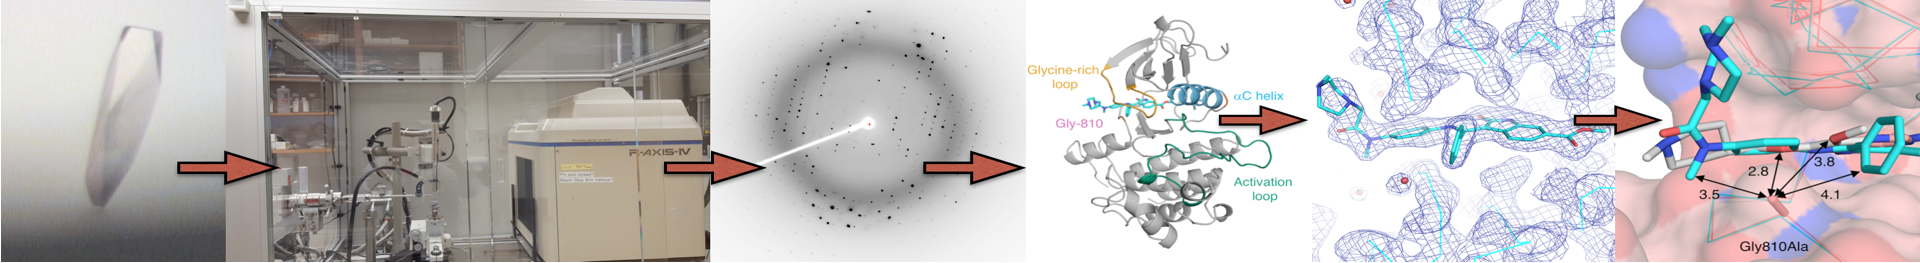
\includegraphics[scale=0.205]{Figures/workflowAB.png}
\end{center}
\vspace{1em}
\Large{
\$HOME/0573crystalDetection
\begin{itemize}
    \item   |--- manu0573.org\footnote{\url{MooersLab/manuscriptInOrg}}
    \item   |--- log0573.org \footnote{\url{MooersLab/modular-writing-project-log-bibtex-org-mode}}
    \item   |--- ./abib0573/abib0573.org\footnote{\url{MooersLab/modular-annotated-bibliography-bibtex-org-mode}}
\end{itemize}
}
\end{frame}
\note{
When I know that I am going to start a writing project, I signed it a number in a database.
I use that number to start the names of the project folder and the key project files.
On the first day my project folder will look like this where there has a manuscript file and the log file that I will be talking about today.
I also have a subfolder for I annotated bibliography that all touch upon near the end of my talk.
}   


\subsection{Templates on MooersLab}
\begin{frame}
\frametitle{Templates at github.com/MooersLab}
\begin{center}
            \begin{figure}
                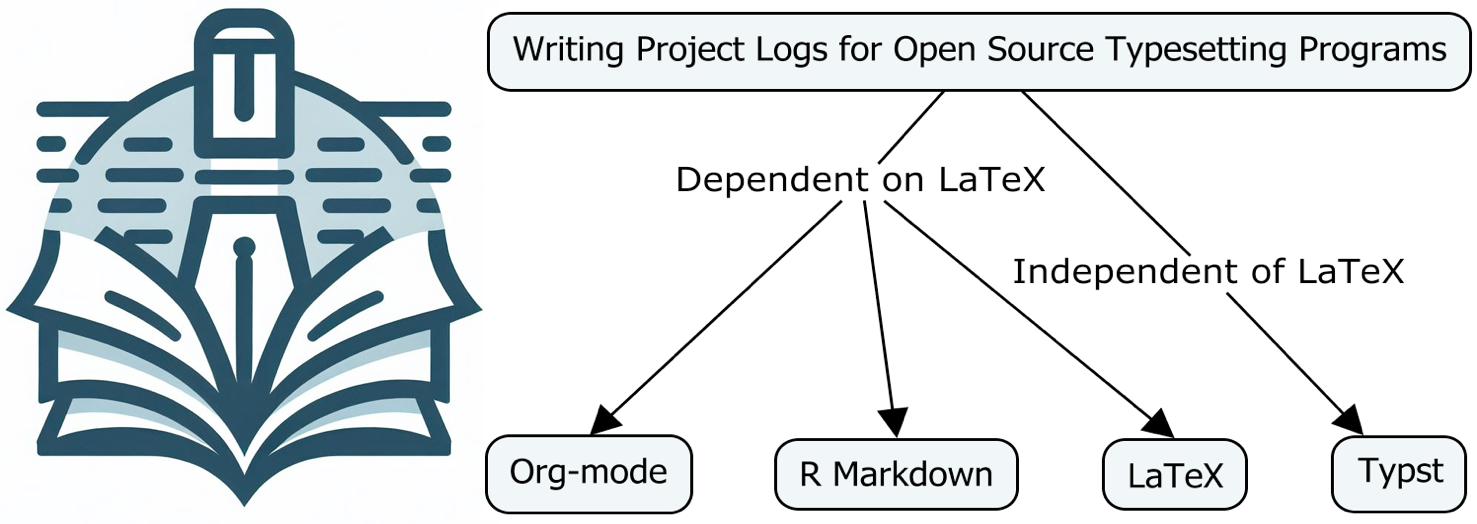
\includegraphics[scale=0.26]{Figures/templates.png}
            \end{figure}
\end{center}
\end{frame}


\subsection{Writing Process}
\begin{frame}
\frametitle{Writing process}
\begin{center}
    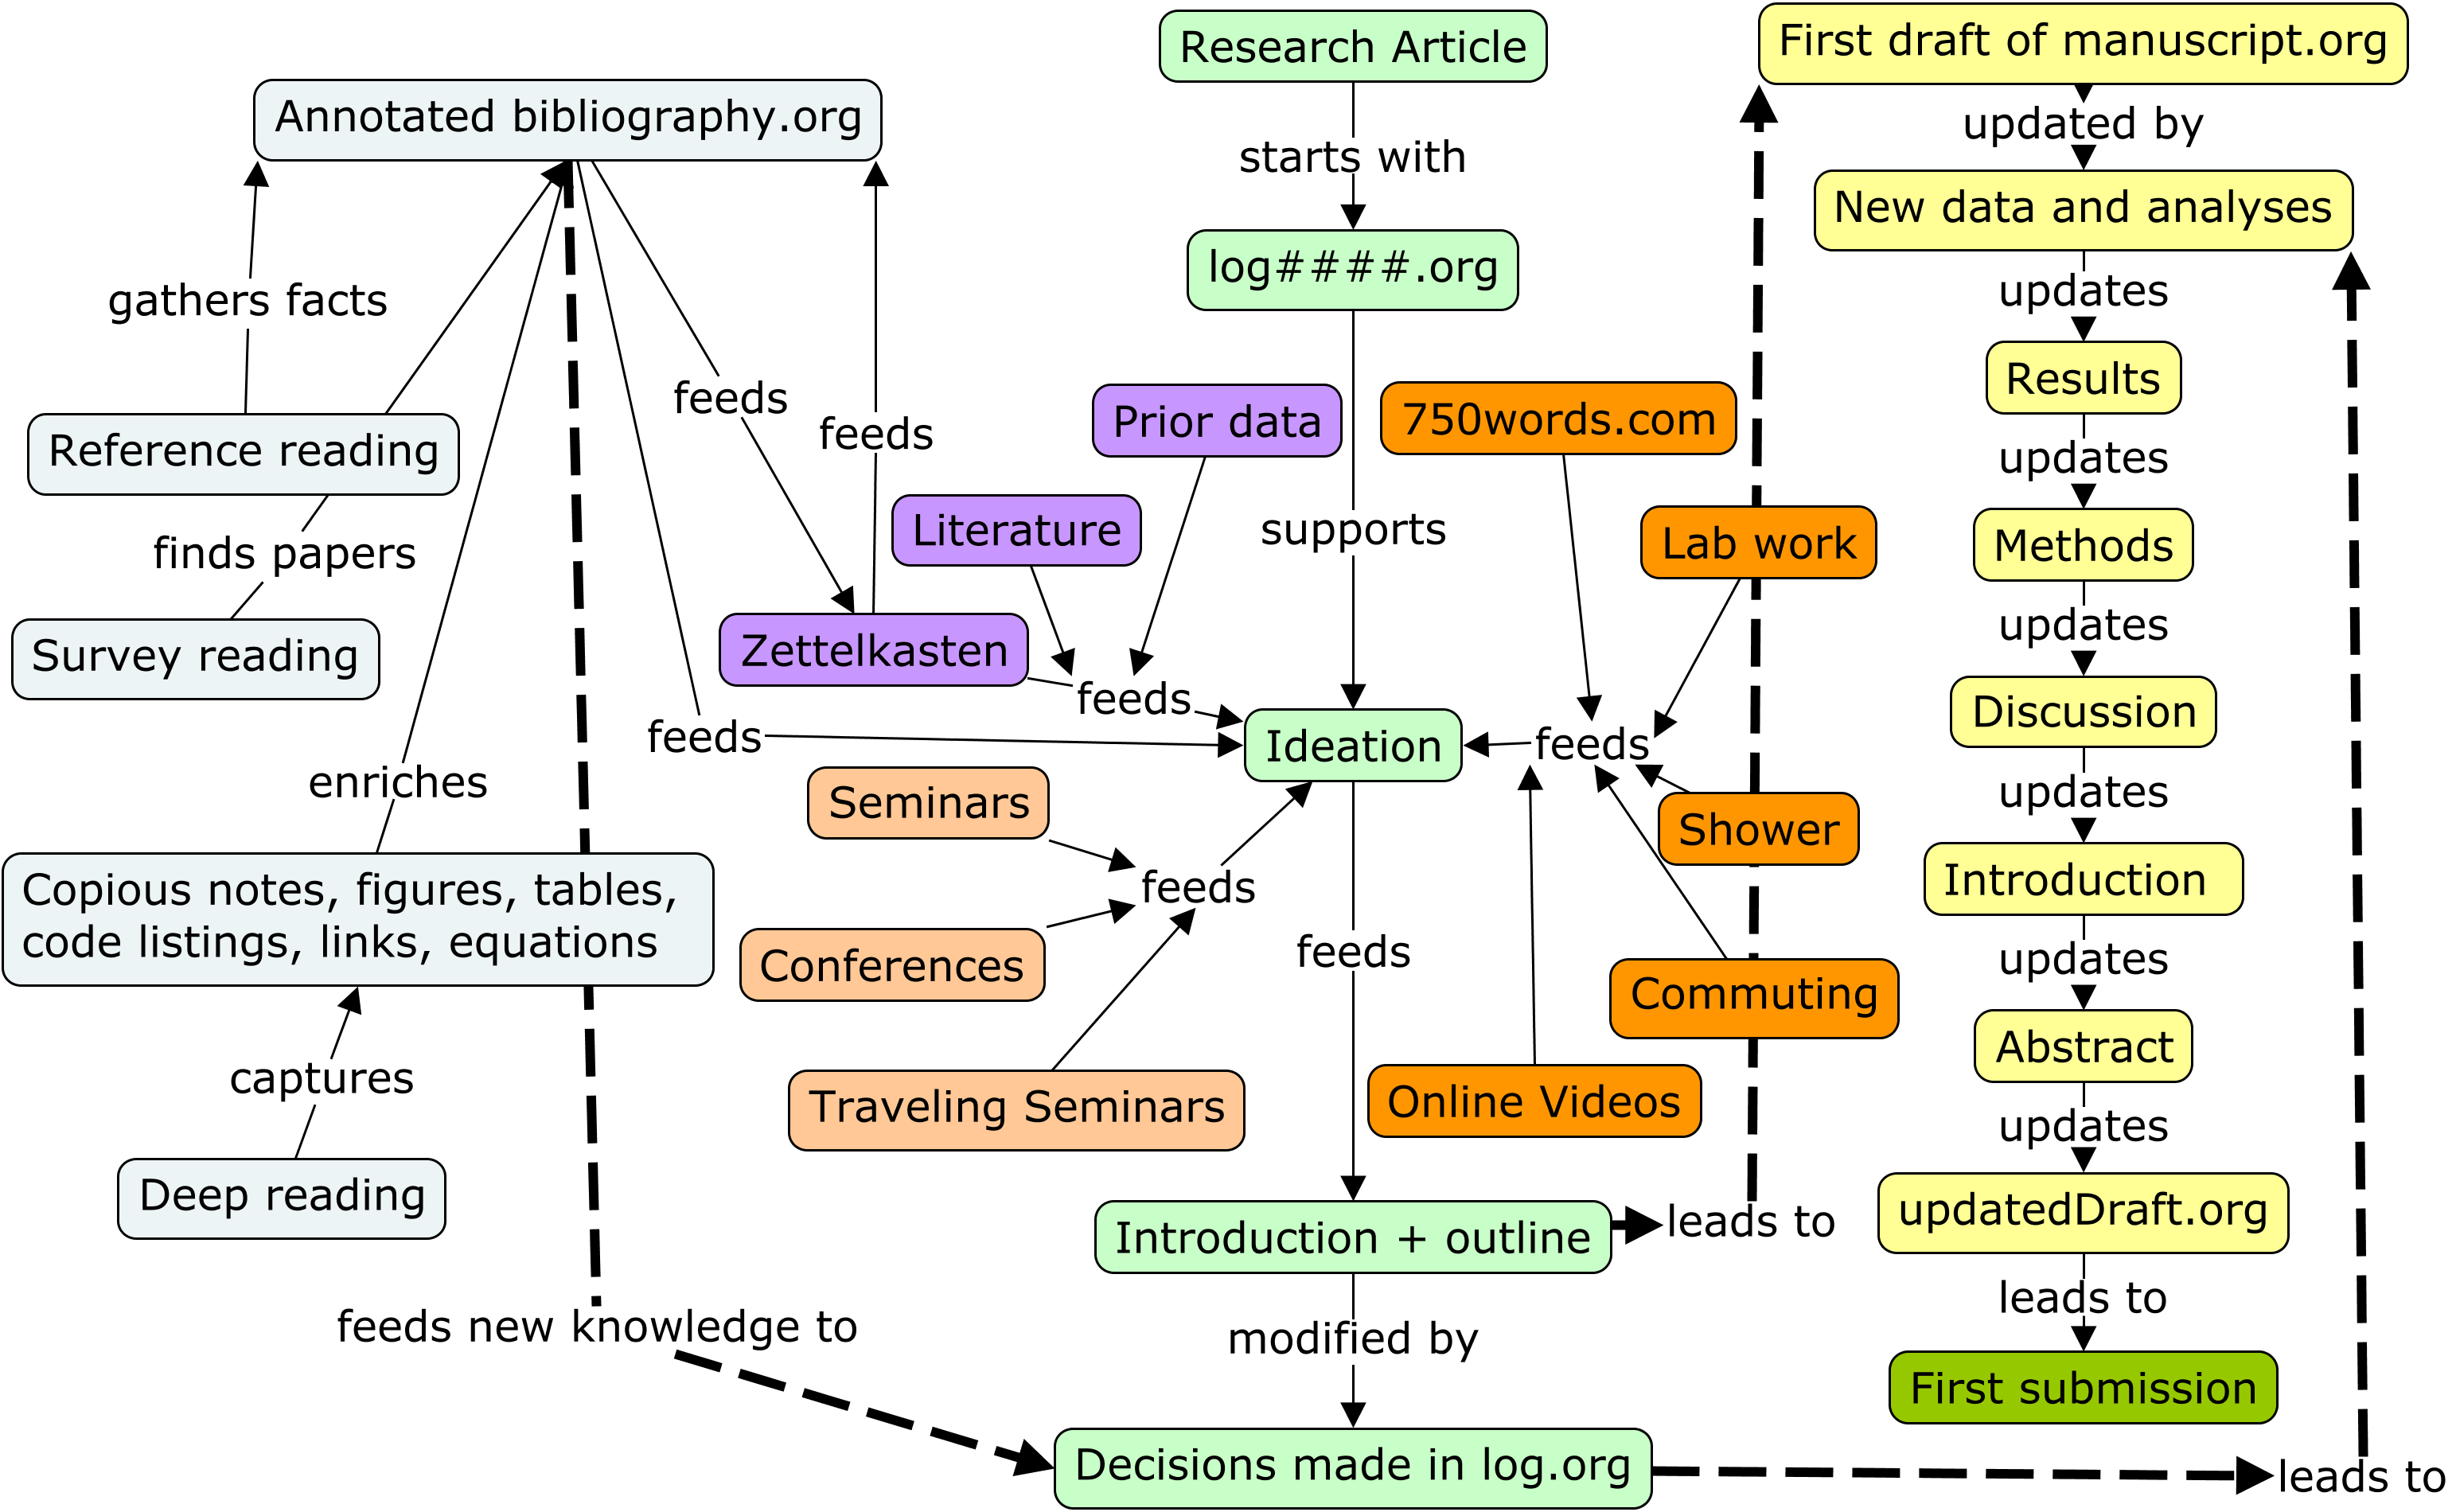
\includegraphics[width=0.8\textwidth, angle=0]{./Figures/writingProcessUpdated}
\end{center}
Made with CmapTools: \url{https://cmap.ihmc.us/}.
\end{frame}
\note{ 
}

\subsection{Goals of Talk}
\begin{frame}
\frametitle{Goals and Outline of Talk}
\Large{
Goals
\begin{itemize}[font=$\bullet$\scshape\bfseries]
\item (re-)Introduce Org Mode.
\item Demystify Emacs some more.
\item Describe research article writing workflow.
\end{itemize}
Outline
\begin{itemize}[font=$\bullet$\scshape\bfseries]
\item Introduce Org Mode. 
\item Introduce Emacs.
\item Walk-through of the writing-project log.
\end{itemize}
}
\end{frame}



% \subsection{Outline of Talk}
% \begin{frame}
% \frametitle{Outline of Talk}
% \Large{
% \begin{itemize}[font=$\bullet$\scshape\bfseries]
% \item Intro to Org Mode and Emacs [VSC, Neorg]
% \item Walk-through of the Templates
% \item Org-capture and Org-roam
% \end{itemize}
% }
% \end{frame}


\section{Main Body of Talk}

\subsection{Features of Org Mode}

\begin{frame}
\frametitle{Features of Org Mode}
\Large{
\begin{columns}
    \begin{column}{0.475\textwidth}
        \begin{itemize}[font=$\bullet$\scshape\bfseries]
        \item Simple markup language
        \item Dynamics tables
        \item README.org on GitHub
           \item Access to LaTeX
            \item Publishing to many formats
            \item Slide shows
            \item Polyglot interactive literate programming in parallel sessions
        \end{itemize}
    \end{column}
    \begin{column}{0.475\textwidth}
        \begin{itemize}[font=$\bullet$\scshape\bfseries]
                    \item Personal knowledge management (org-roam)
            \item Wiki and Web Page building
            \item Blogging
            \item Journaling
            \item Time-logging
            \item Time management (org-agenda)

        \end{itemize}
    \end{column}
    \end{columns}
   }
\end{frame}
\note{

}


\begin{frame}
\frametitle{Talk about Org Mode by the developer}
\begin{center}
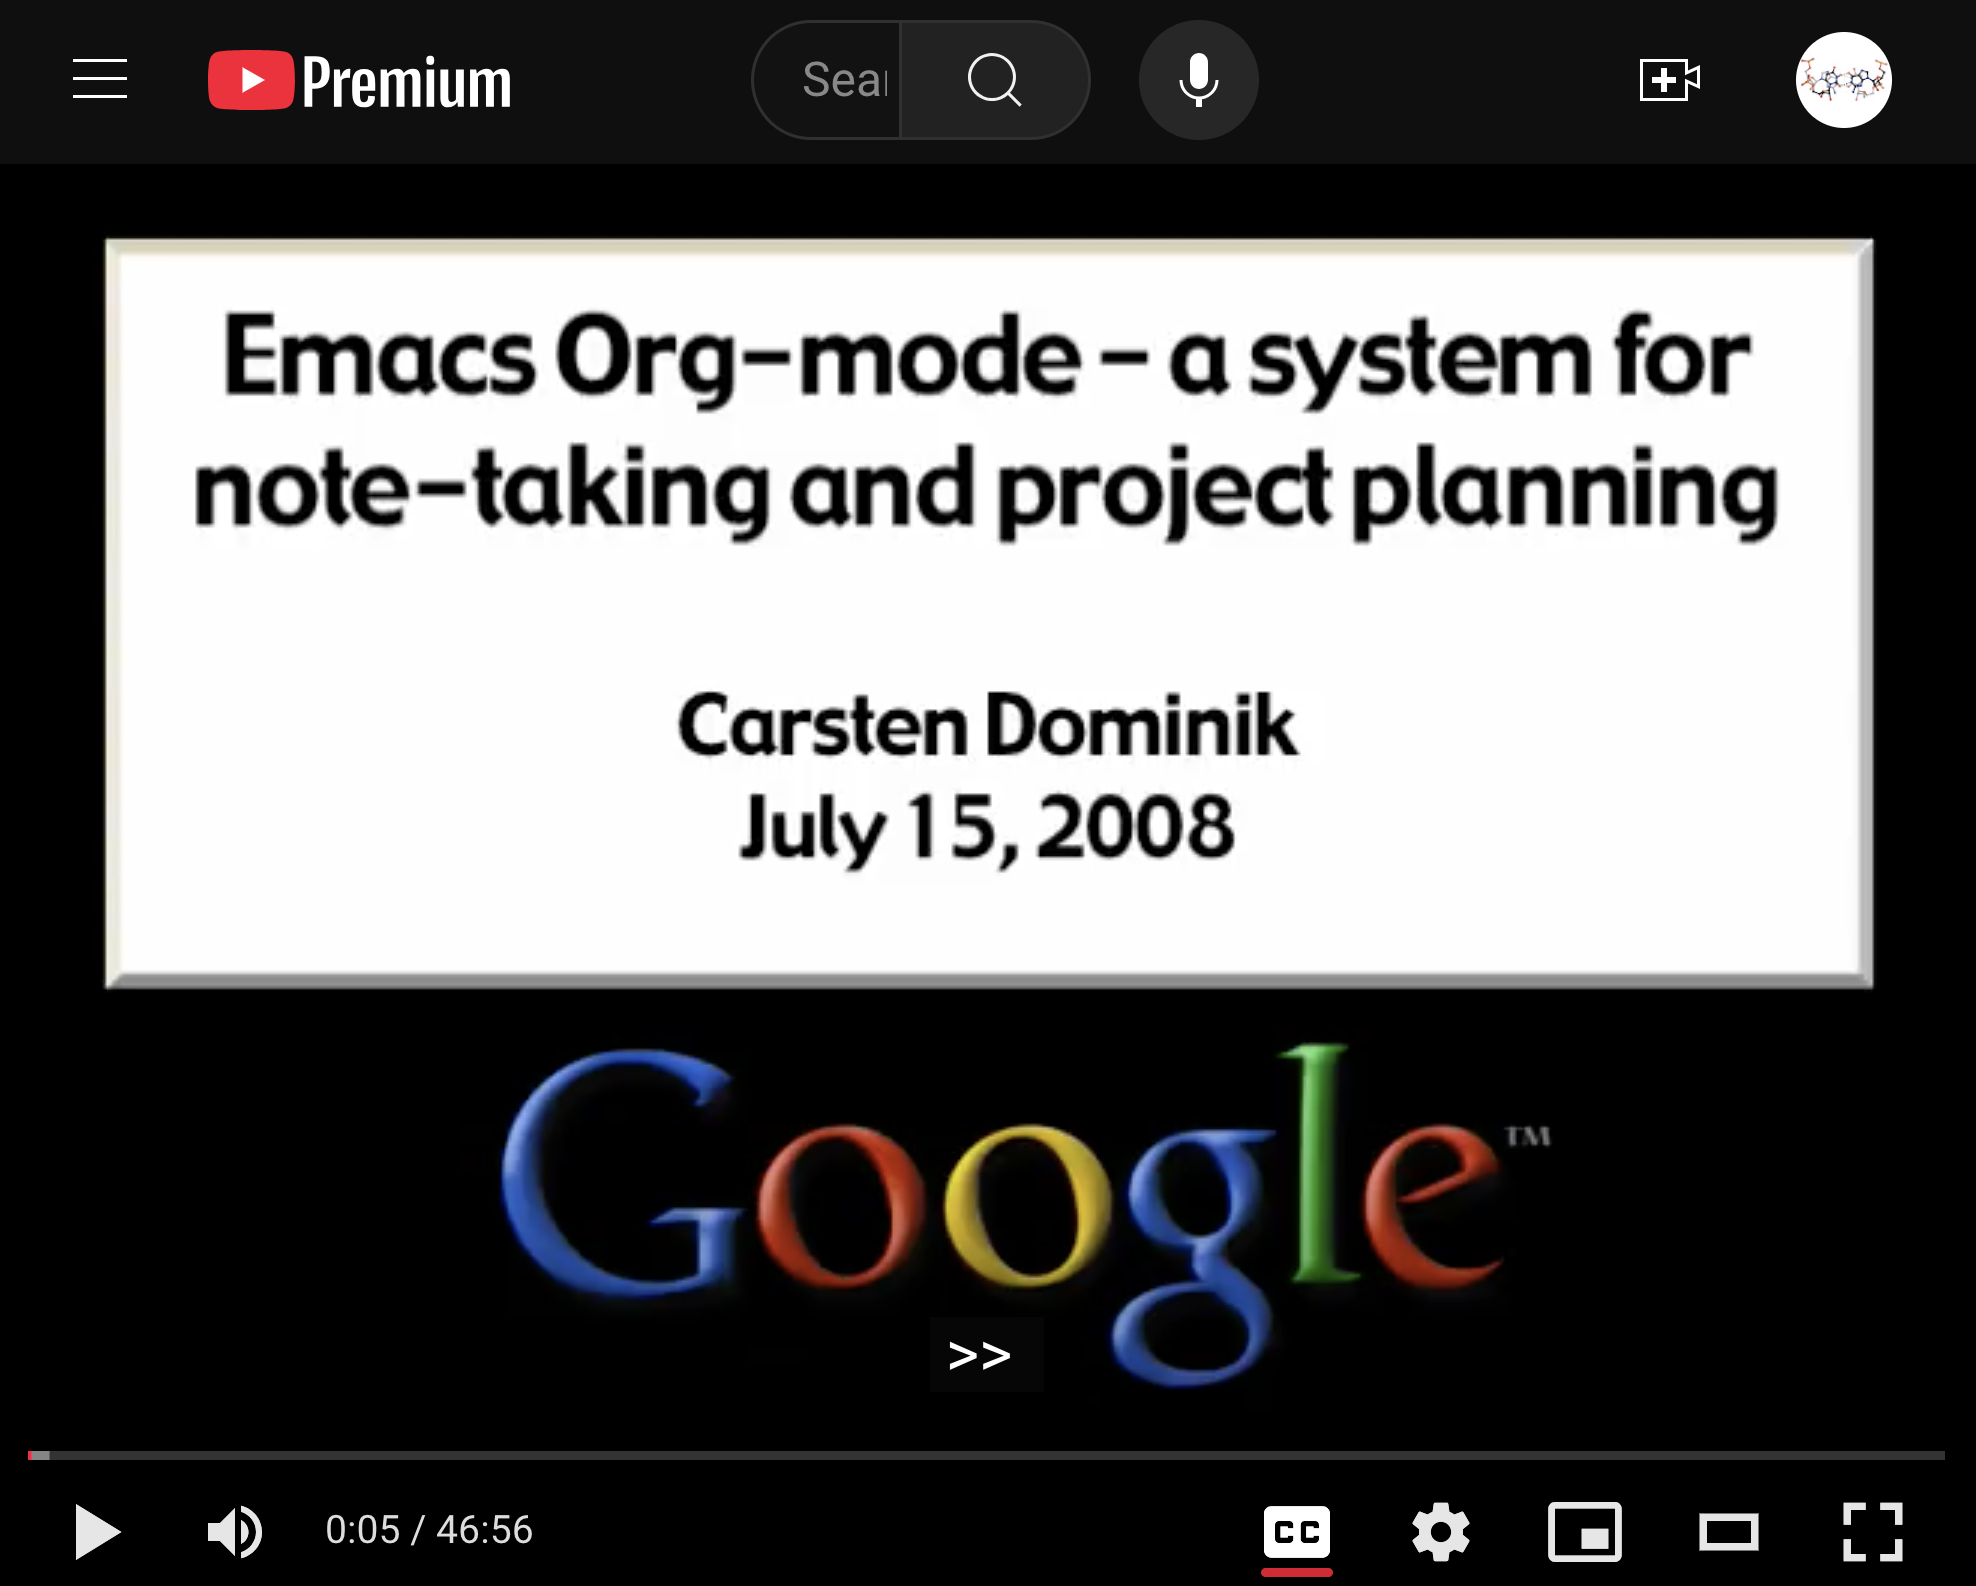
\includegraphics[scale=0.2]{Figures/Carsten2008.png}
\end{center}
\url{https://www.youtube.com/watch?v=oJTwQvgfgMM}
\url{https://staff.science.uva.nl/c.dominik/\#org60c8666}
\end{frame}
% Bernt Hansen.
% https://doc.norang.ca/org-mode.html





% https://karl-voit.at/2017/09/23/orgmode-as-markup-only/

% https://doc.norang.ca/org-mode.html




% \subsubsection{Editors for Org Mode}
% \begin{frame}
% \frametitle{Editors for Org Mode}
% \begin{itemize}
% \item VS Code
%     -
%     -
%     -
    
% \item Neorg
% \item Emacs 
%     - built-in as of Version 29
%     - org-agenda
%     - org-roam
% \end{itemize}
% \end{frame}



% https://github.com/karlicoss/orgparse
\subsubsection{Installing GNU Emacs}
\begin{frame}
\frametitle{Installing GNU Emacs}
\Large{
\begin{center}
\begin{itemize}[font=$\bullet$\scshape\bfseries]
    \item Installed already?
    \item Package manager: Homebrew, Macports, Anaconda.
    \item Binary download \footnote{\url{https://www.gnu.org/software/emacs/download.html}}.
    \item Compile from source\footnote{\url{https://github.com/MooersLab/compile-emacs-29}}.
\end{itemize}
\end{center}
}
\end{frame}


\subsubsection{Typical Emacs User}
\begin{frame}
\frametitle{Interview of an Emacs user (not for newbies)}
\begin{center}
    
\includegraphics[scale=0.5]{Figures/EmacsUser.png}
\end{center}
\url{https://www.youtube.com/watch?v=urcL86UpqZc&t=5s}
\end{frame}





\subsubsection{Terminal vs GUI (emacs)}
\begin{frame}
\frametitle{Terminal (emacs -nw) vs GUI (emacs)}
\begin{center}
    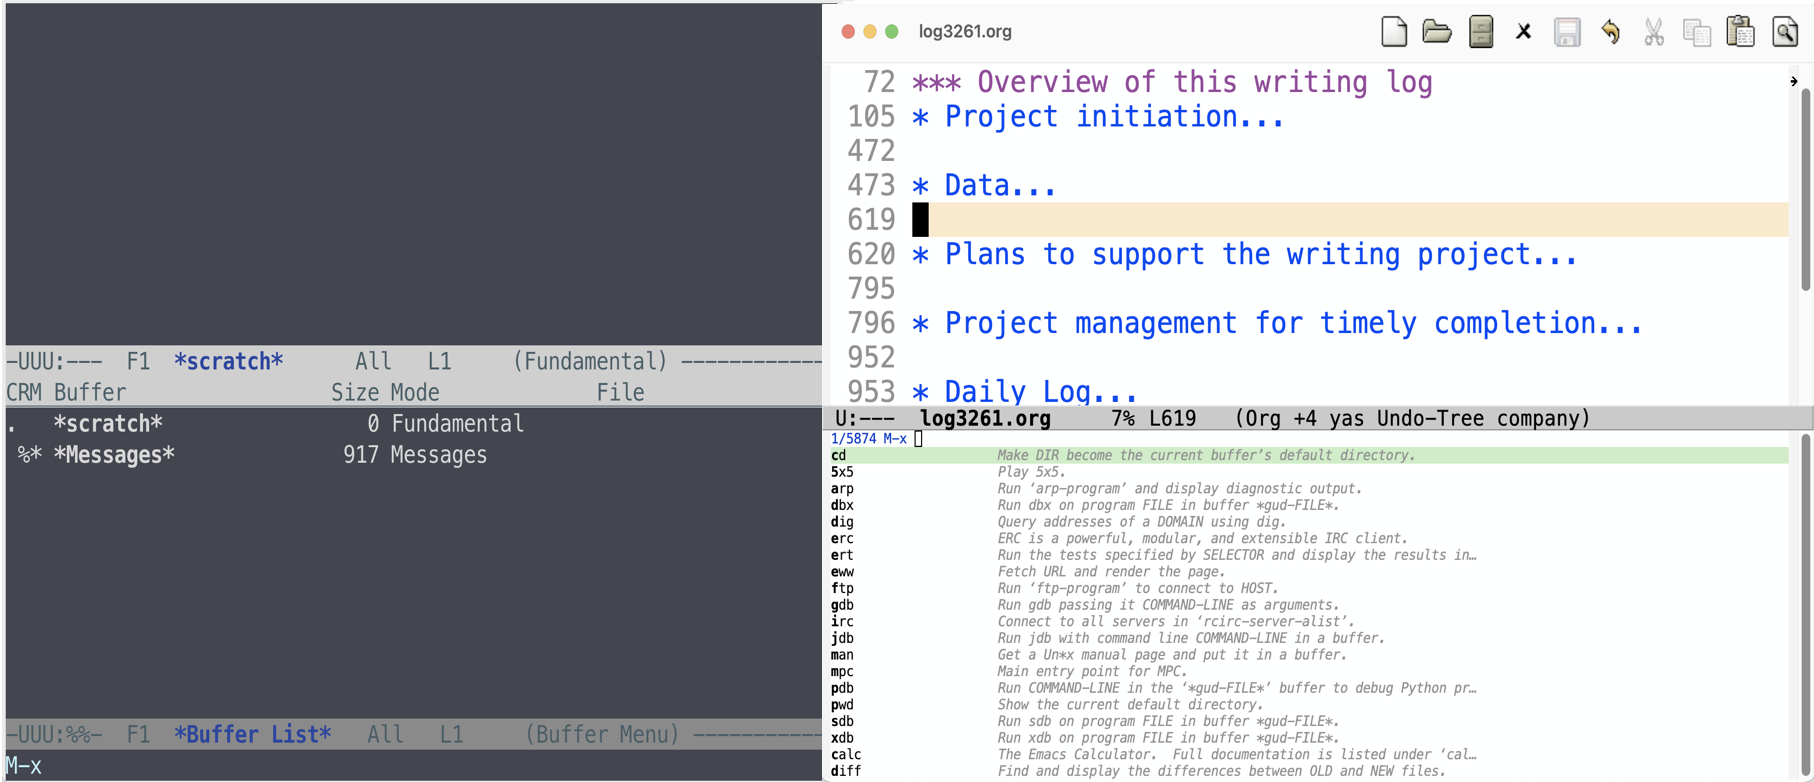
\includegraphics[scale=0.43]{Figures/EmacsInterfaces.png}
\end{center}
Left: 2 buffers, 2 modelines, 1 minibuffer; Right: 1 buffer, 1 modeling, 1 minibuffer with vertico.
\end{frame}


\subsubsection{Terminal Emacs}
\begin{frame}
\frametitle{Emacs at top, Schooner in bottom tmux pane}
\begin{center}
    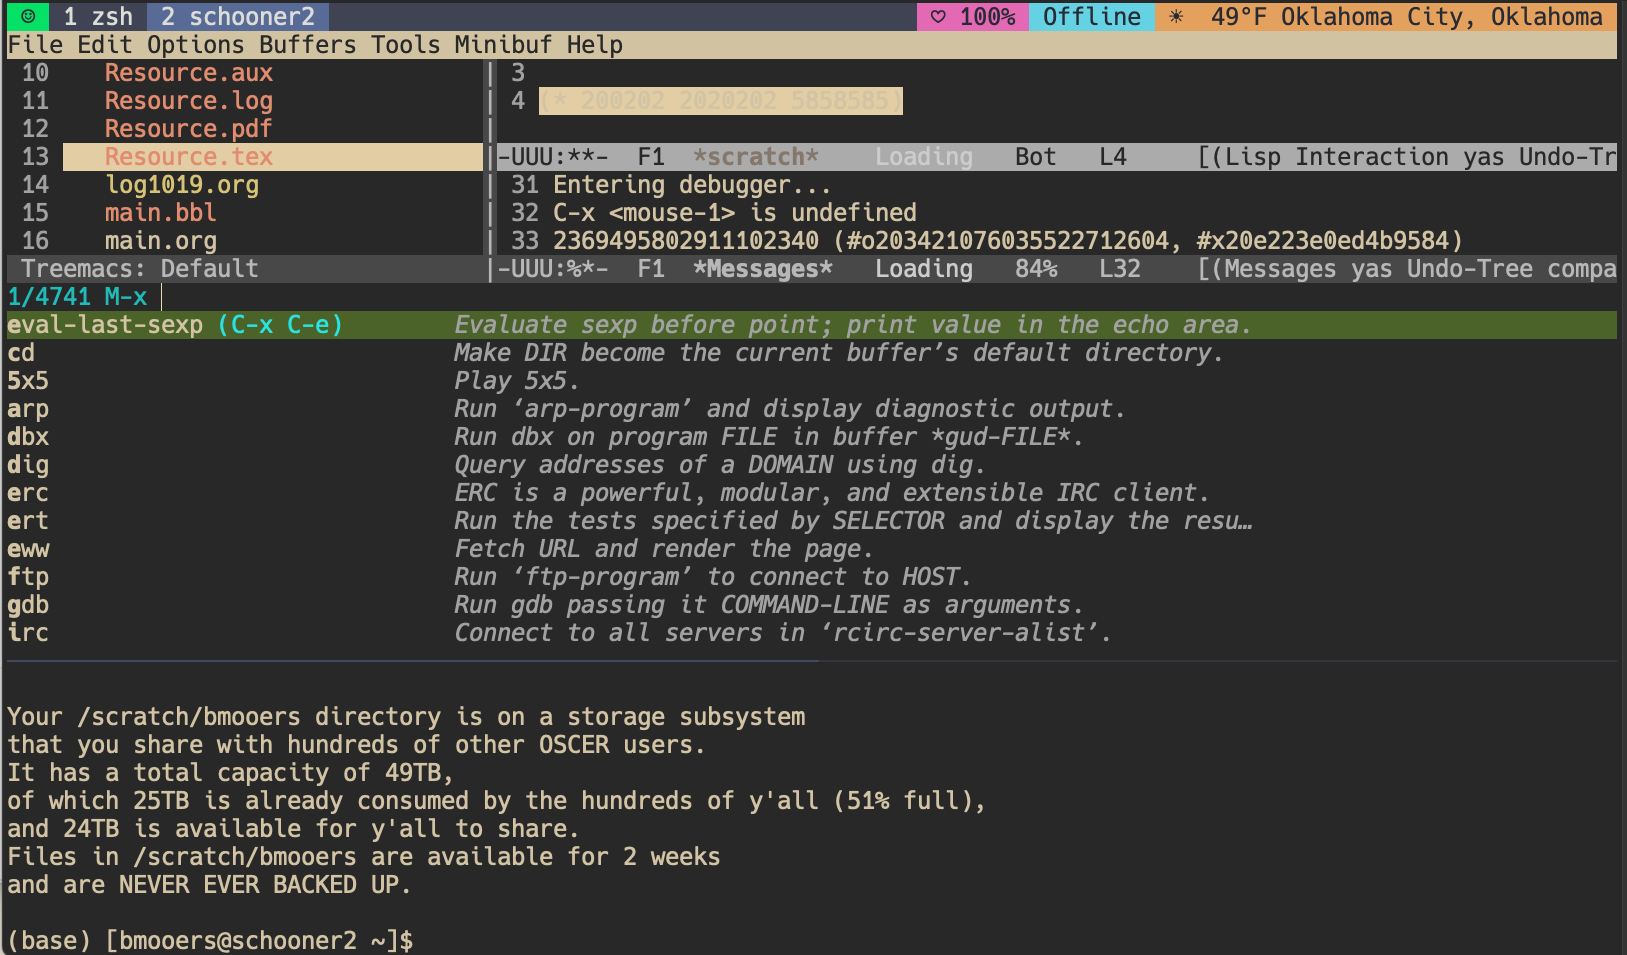
\includegraphics[scale=0.2]{Figures/EmacsSchooner.png}
\end{center}
C-h, C-j, C-k, C-l \url{https://github.com/laishulu/emacs-tmux-pane}
\end{frame}


\subsubsection{File pulldown menu}
\begin{frame}
\textbf{Meta key (M) = Alt key; C, control;} S, shift; s, super (left-option); H, hyper (right-option)
\frametitle{File pulldown menu}
\begin{center}
    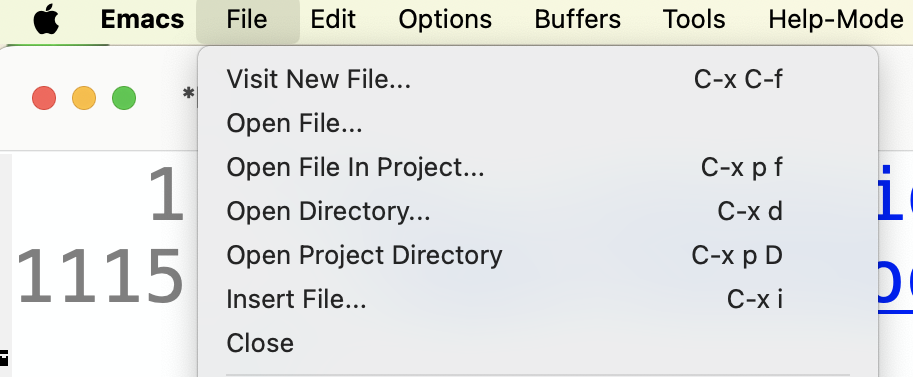
\includegraphics[scale=0.85]{Figures/filePulldownCropped.png}
\end{center}
\end{frame}


\subsubsection{Org menu visible only in org-mode}
\begin{frame}
\frametitle{Org pulldown menu}
\begin{center}
    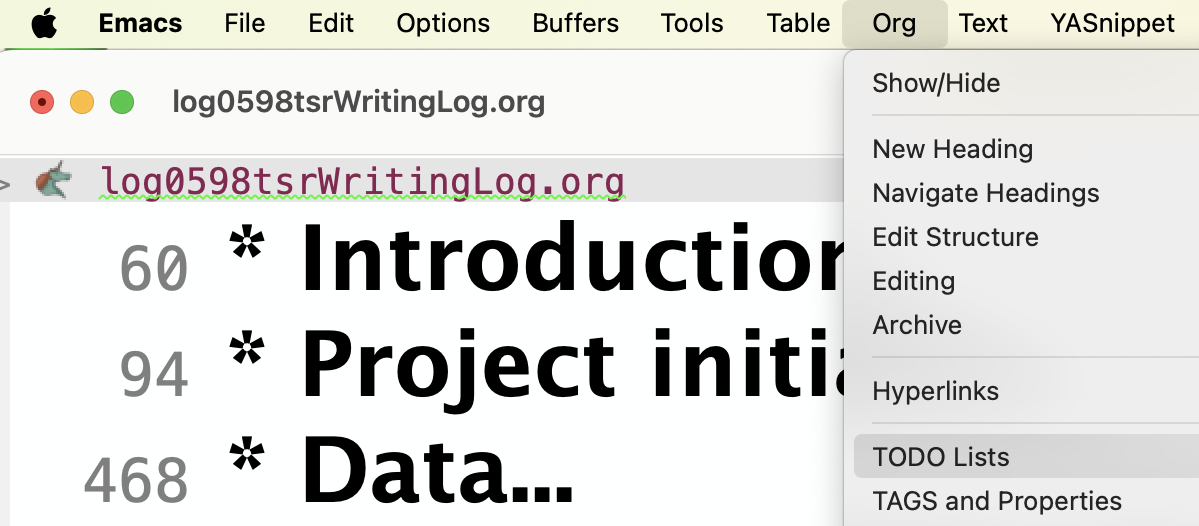
\includegraphics[scale=0.7]{Figures/orgPulldownCropped.png}
\end{center}
\end{frame}



\subsubsection{Key-bindings}
\begin{frame}
\frametitle{Basic key-bindings}
\Large{
\begin{center}
\begin{itemize}[font=$\bullet$\scshape\bfseries]
    \item C-g  ;;undo last command
    \item C-x C-f ;;find file  C-x C-s ;;save file     C-x C-w ;;write file
    \item C-1 ;; close current buffer (and file)  C-x 1  close other buffers
    \item C-x C-b  ;; generate list of open buffers
    \item C-x C-c  ;; quit Emacs
    \item C-x C-e  ;; run elisp symbolic expression
    \item C-h ? ;; help commands   C-h b ;; show active key bindings
    \item C-h R org ;; open the Org-manual; C-h t ;; open tutorial
    \item M-x some command in the minibuffer
\end{itemize}
\end{center}
}
\end{frame}


\subsubsection{}
\begin{frame}
\frametitle{}
\begin{center}
    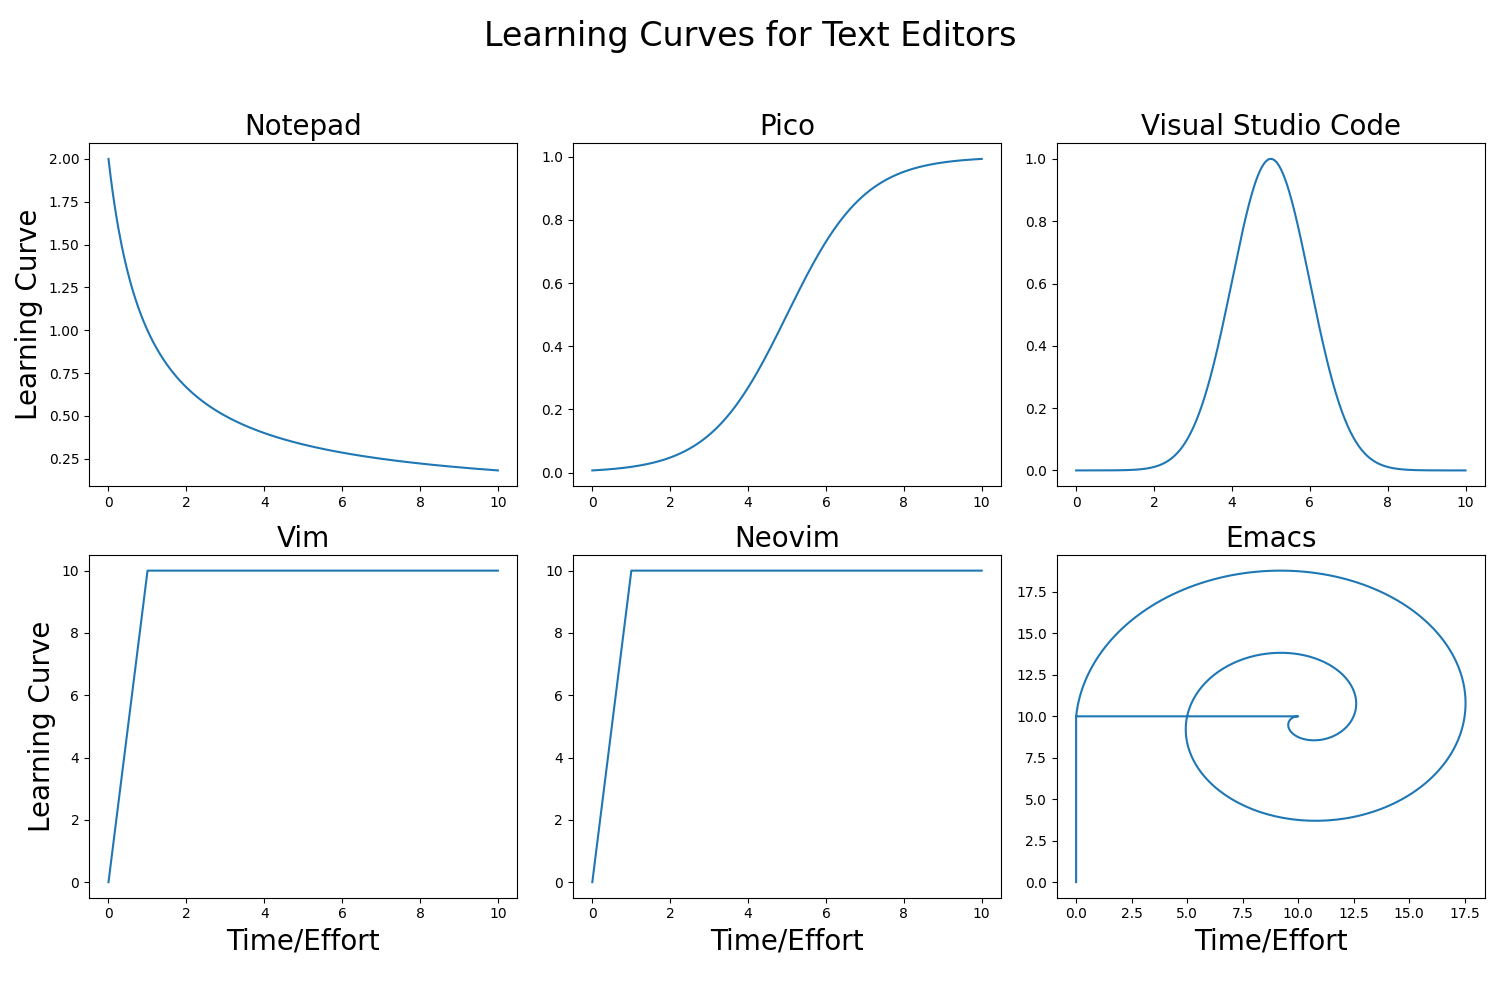
\includegraphics[scale=0.34]{Figures/learning_curves.png}
\end{center}
\end{frame}





\subsubsection{Org manual}
\begin{frame}
\frametitle{Open org manual: C-h R org}
\begin{center}
    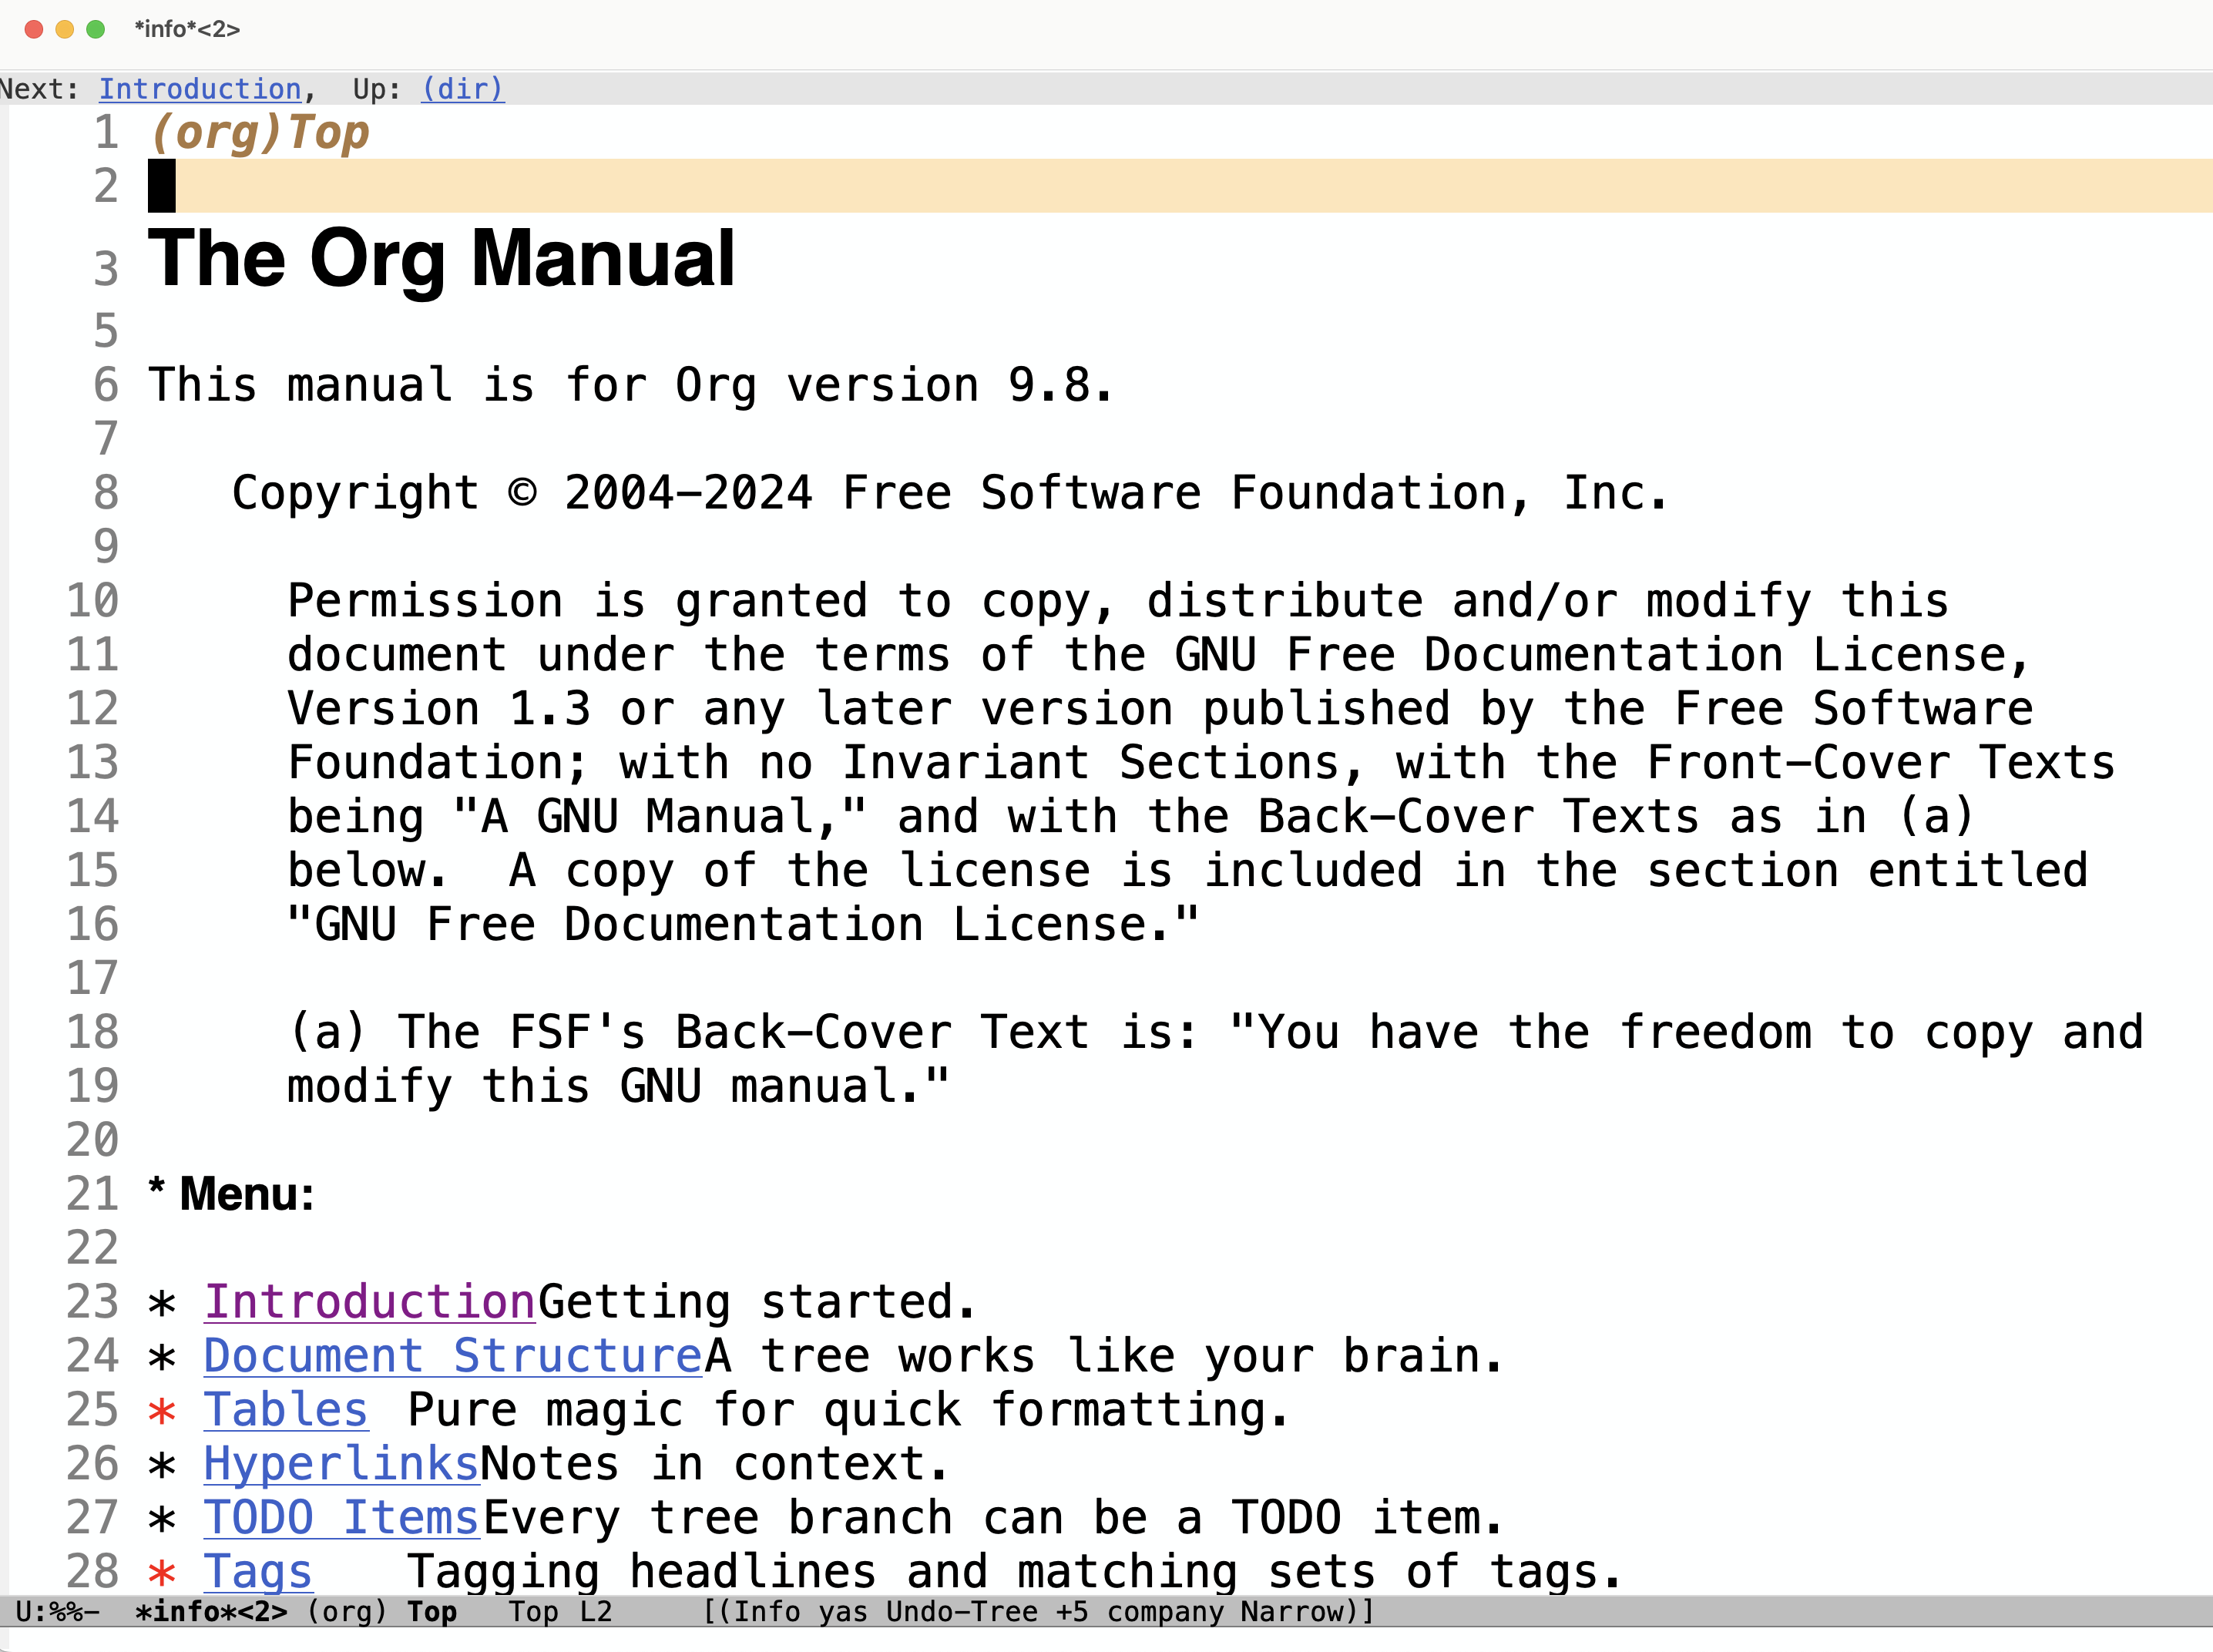
\includegraphics[scale=0.2]{Figures/orgManual.png}
\end{center}
\end{frame}




\subsubsection{Emacs configuration folder}
\begin{frame}
\frametitle{Emacs configuration folder }
Traditionally: \$HOME/.emacs.d ;; Not necessary to hide folder.
\begin{center}
    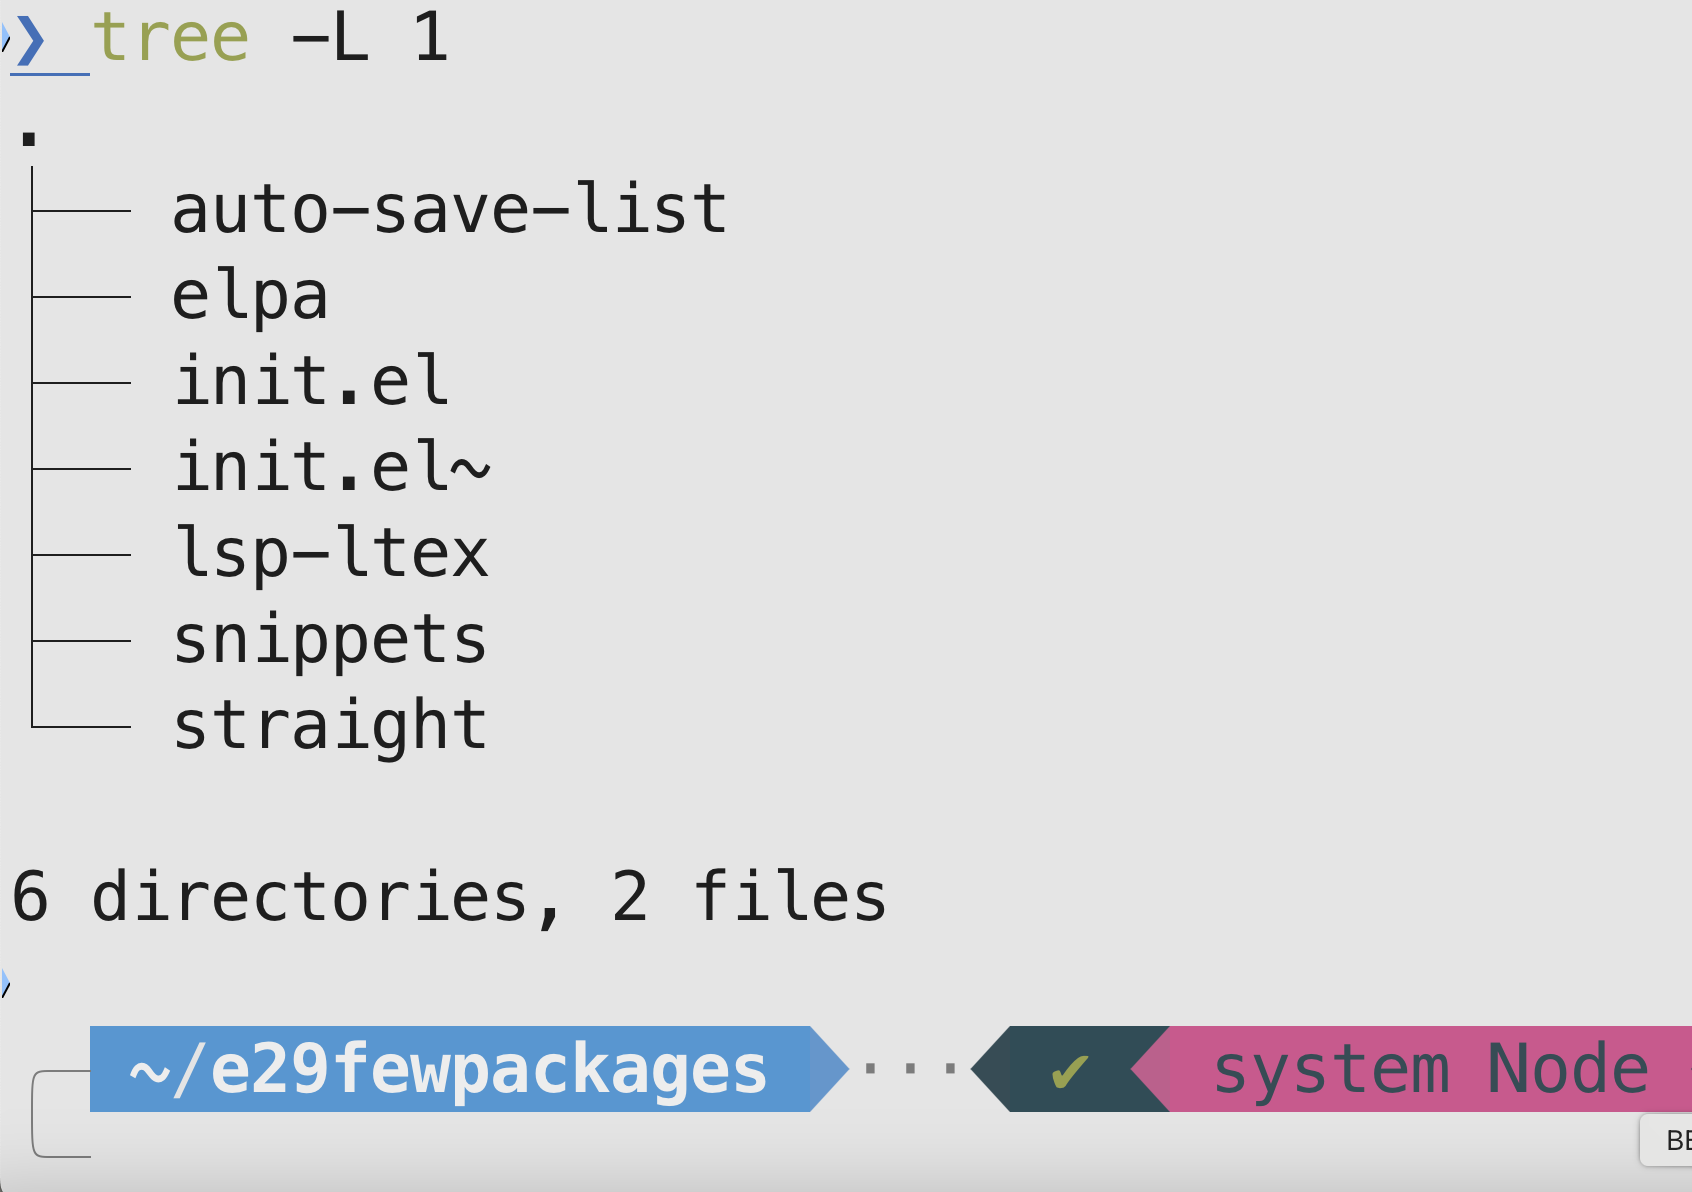
\includegraphics[scale=0.28]{Figures/tree.png}
\end{center}
alias efnw='/Applications/Emacs29.4.app/Contents/MacOS/Emacs -nw --init-directory ~/e29fewpackages'
\end{frame}


\subsubsection{Top of init.el file}
\begin{frame}
\frametitle{Top of init.el file }
\begin{center}
    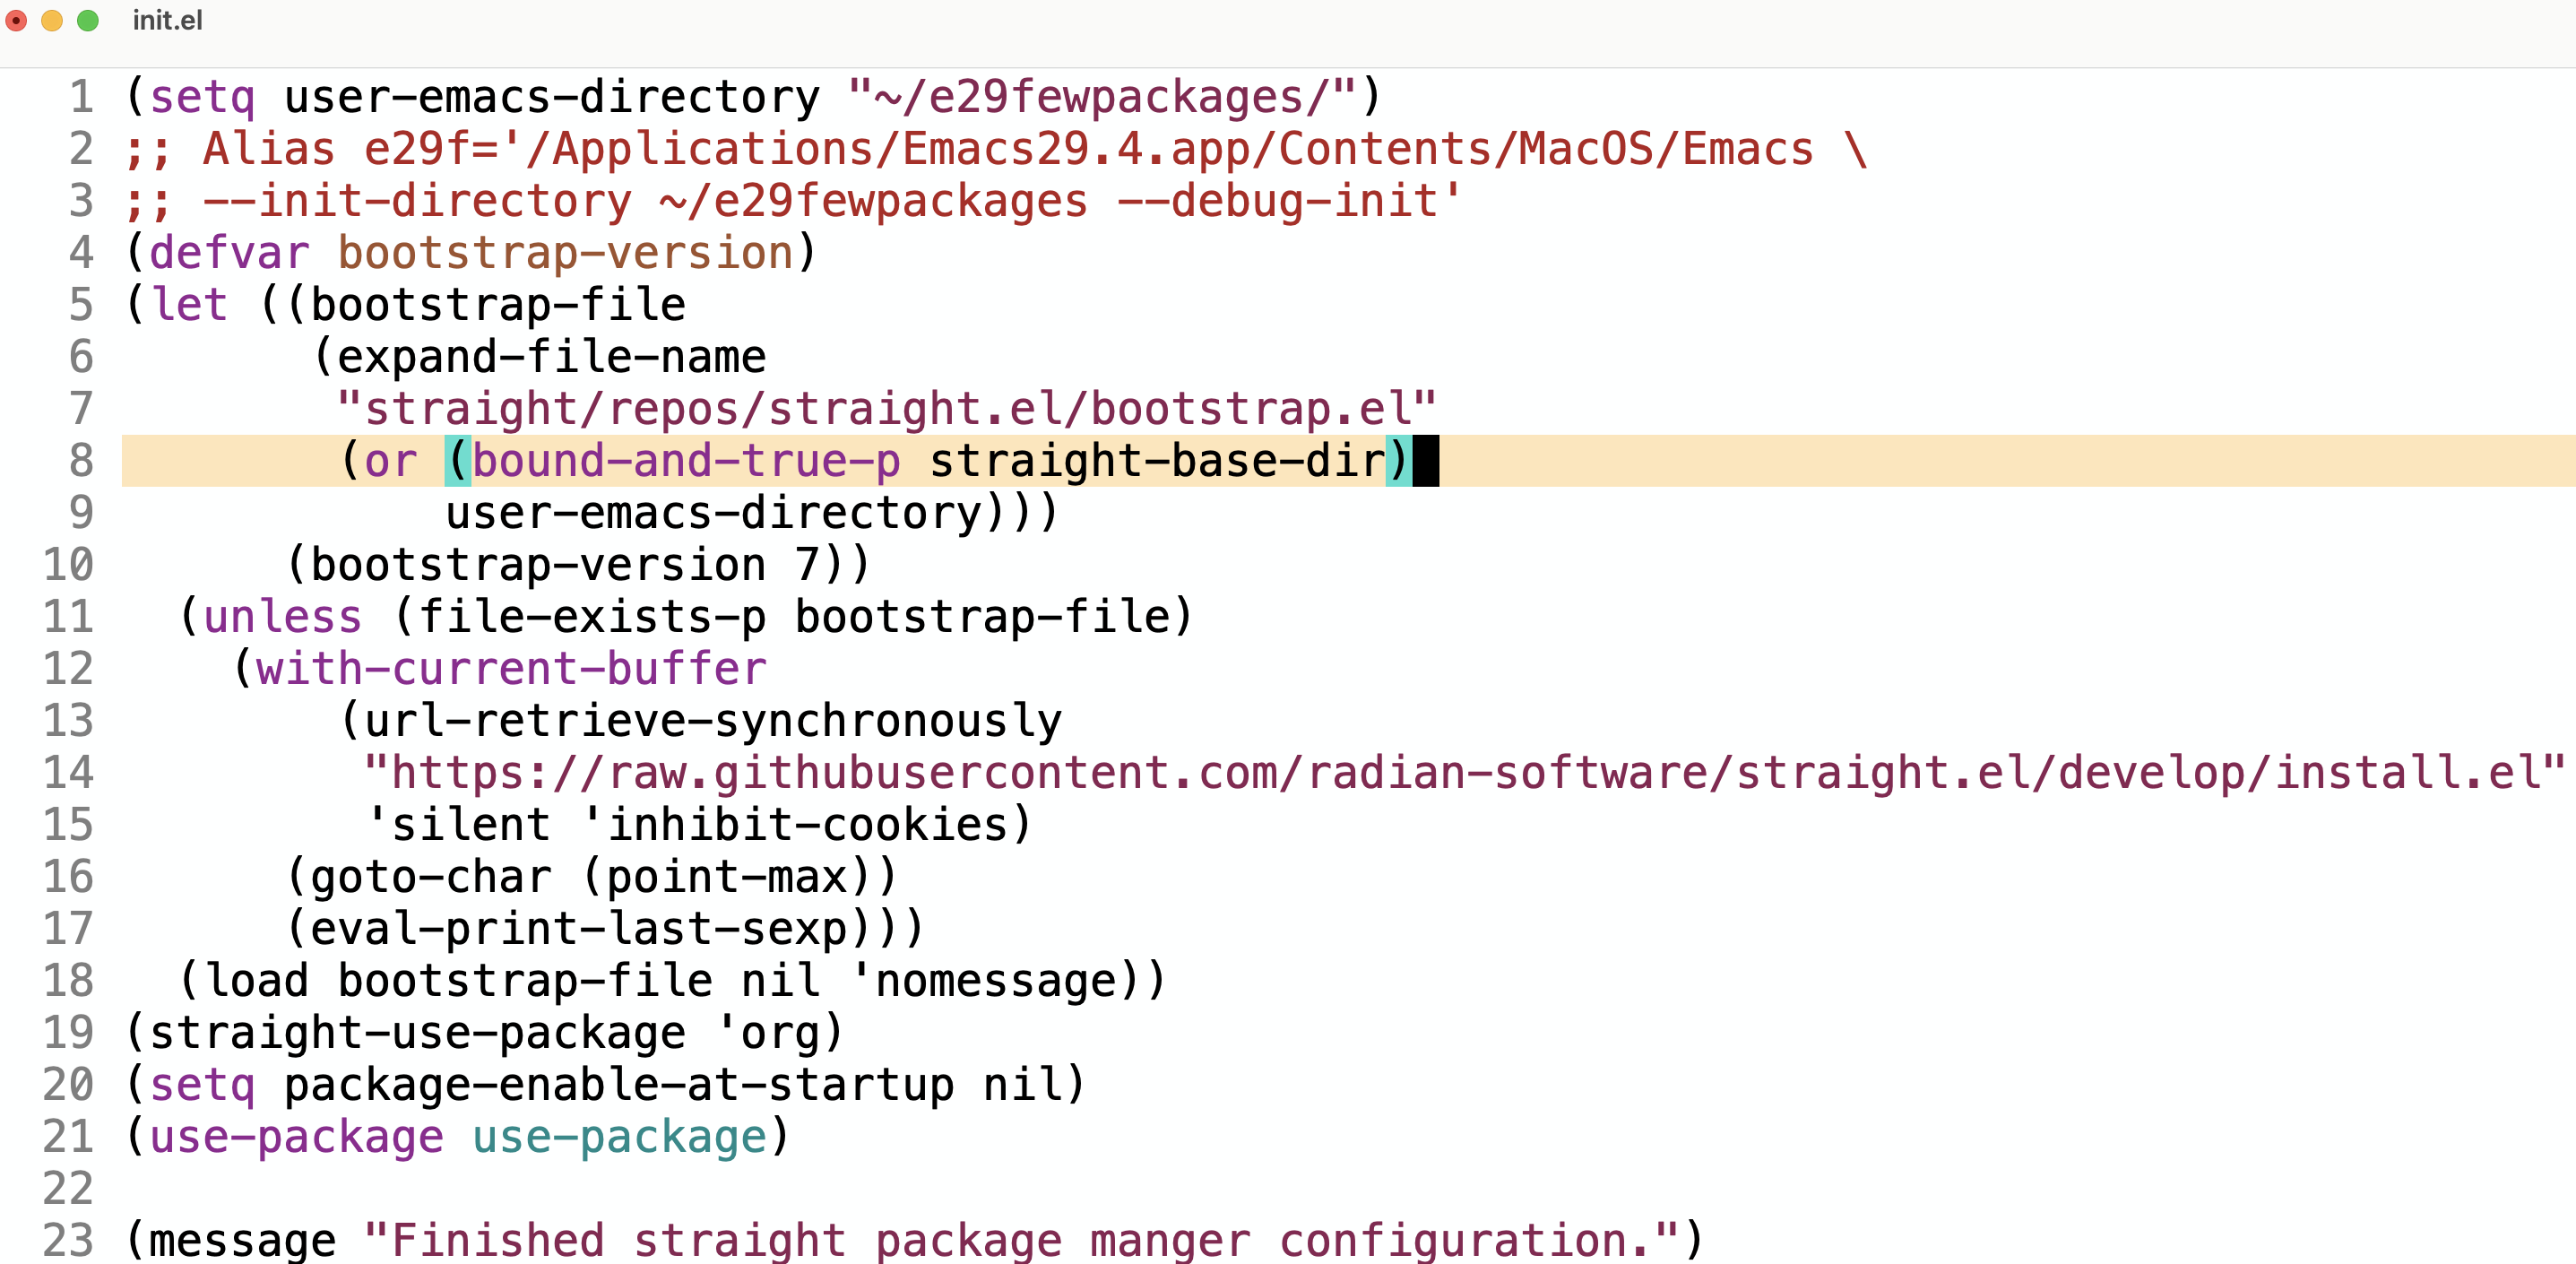
\includegraphics[scale=0.25]{Figures/initFile.png}
\end{center}
\url{github.com/MooersLab/dsw-2024-org-mode-init}
\end{frame}


\subsection{Manuscript}

% \subsubsection{Overview of the Manuscript file}
% \begin{frame}
% \frametitle{Overview of the Manuscript file}
% \end{frame}


\subsubsection{Overview of the manuscript.org}
\begin{frame}
\frametitle{Overview of the manuscript.org}
\begin{center}
    
\includegraphics[width=0.7\textwidth, angle=0]{./Figures/manuscriptOverview.png}
\end{center}
\end{frame}
\note{
This is the overview that you are provided with in your first opened up the generic manuscript template in org-mode.
There is a startup keyword near the top of the file that has the overview command which provides this collapse view or the manuscript.
All the major headings have been folded up.
I have opened up the abstract guidance heading.
Below it is what is known as a drawer.
Because the line above has this no export keyword between a pair of colons, the guidance will not be exported to the PDF.
By putting the cursor on the word guidance between the paracolons and hitting tab, I am able to close the drawer or open it.
The lines that start with a pound sign for the bike plus sign are org-mode commands.
By using the lactic variant, actually able to utilize lactic commands.
Some look Tech commands are directly recognized my org-mode and you do not need this prefix.
The remaining commands require this prefix.

I would I now want to bring your attention to the drawer near the top called the preamble.
This is analogous to the Preamble section of a latex file.
It has the prefix of  \LaTeX _ header.
This allows us to import library files and execute commands that control the appearance of the PDF.
}

\subsubsection{Preamble of the manuscript.org}
\begin{frame}
\frametitle{Preamble of the manuscript.org}
\begin{center}
    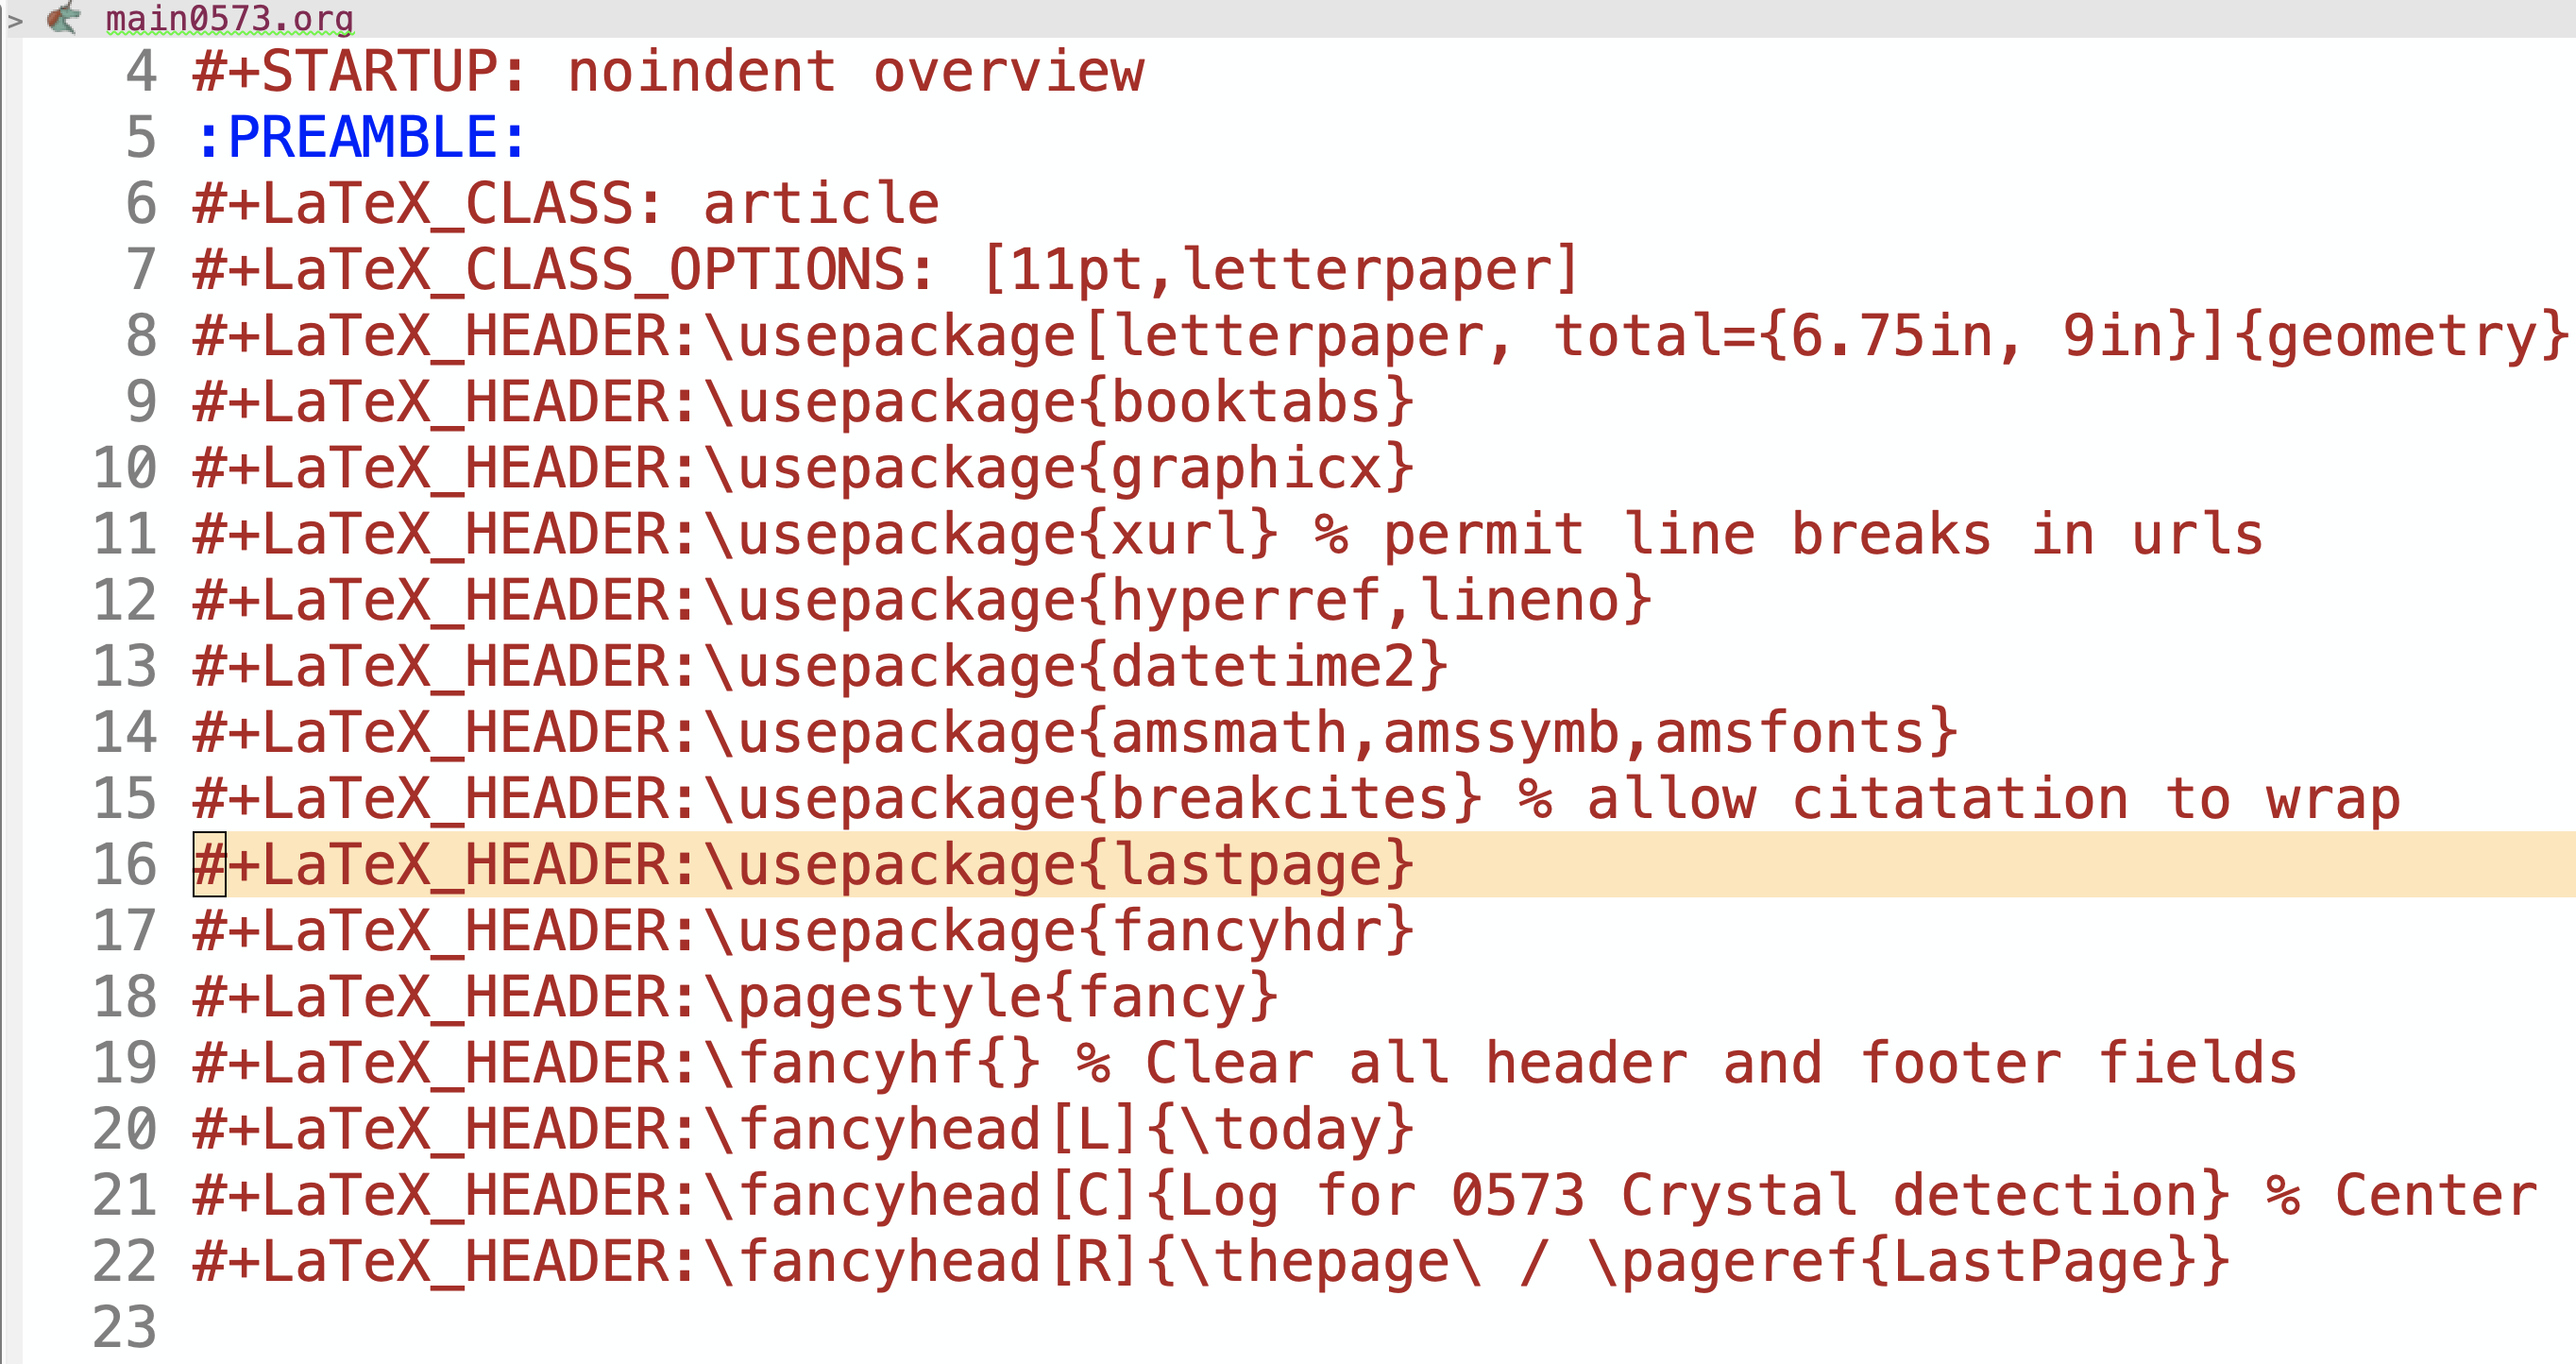
\includegraphics[width=0.98\textwidth, angle=0]{./Figures/manuscriptPreamble.png}
\end{center}
\end{frame}
\note{

}



\subsubsection{Title page of classic manuscript}
\begin{frame}
\frametitle{Title page of first-submission manuscript}
\begin{center}
    
\includegraphics[width=0.8\textwidth, angle=0]{./Figures/manuscriptTitle.png}
\end{center}
\url{https://github.com/MooersLab/manuscriptInOrg}
\end{frame}



\subsubsection{Second page}
\begin{frame}
\frametitle{Second page}
\begin{center}
    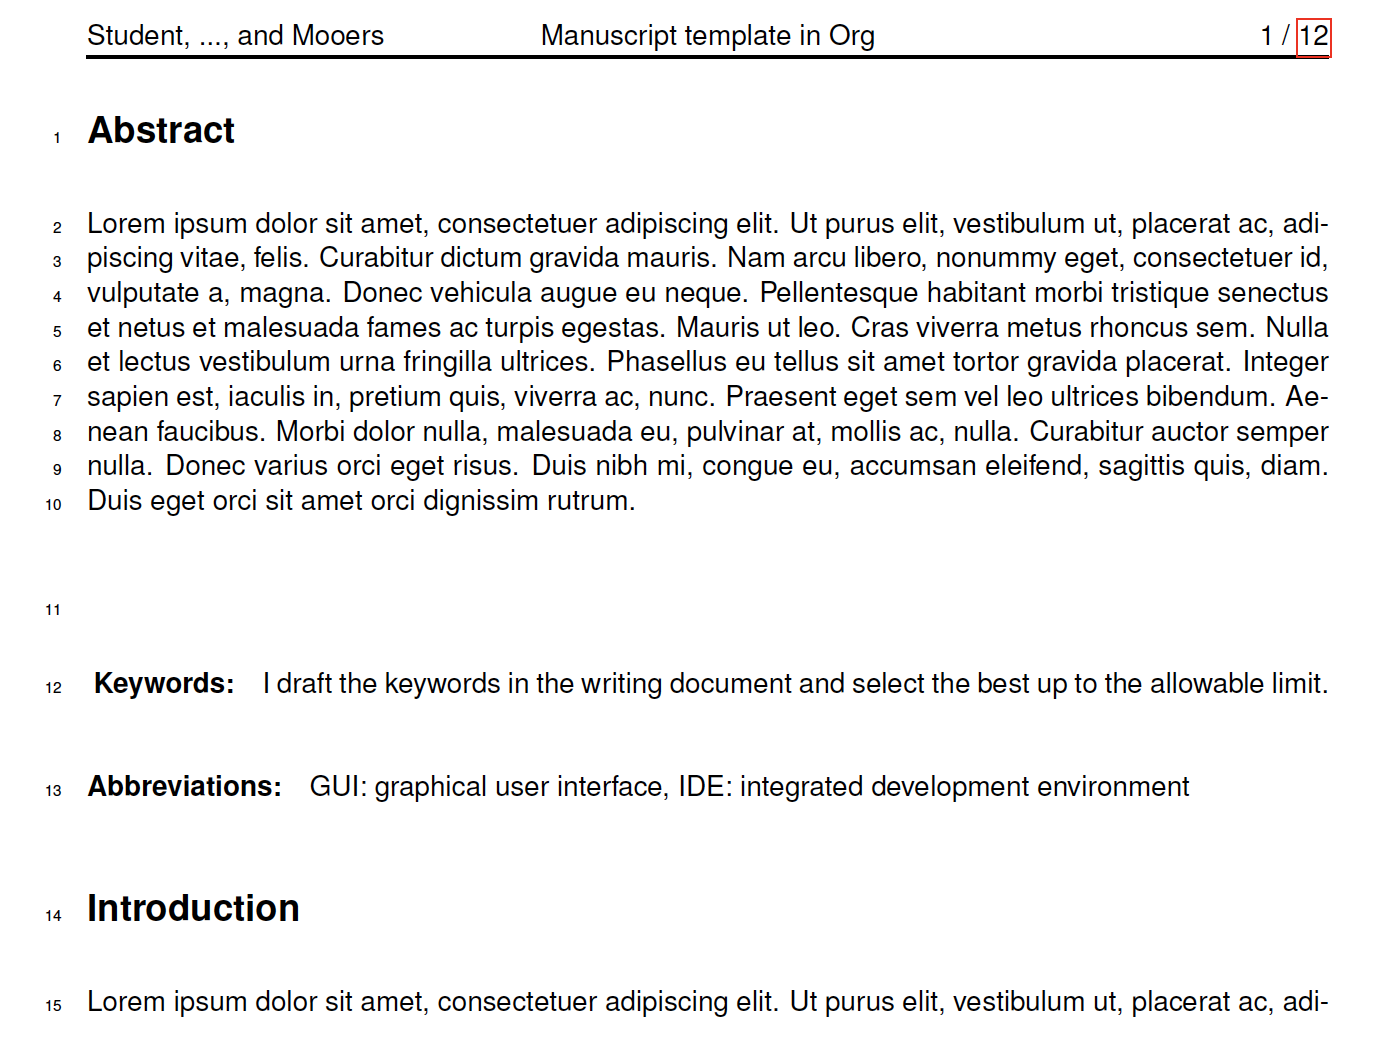
\includegraphics[width=0.94\textwidth, angle=0]{./Figures/manuscriptSecondPage.png}
\end{center}
\end{frame}

\subsubsection{The problem}
\defverbatim[colored]\exampleCodeC{
\large{
\begin{pythoncode}
    @Article{Mooers2020ShortcutsForFasterImageCreationInPyMOL,
      author       = {Mooers, Blaine HM},
      pages        = {268--276},
      title        = {Shortcuts for faster image creation in PyMOL},
      volume       = {29},
      number       = {1},
      annote       = {The seminal paper on PyMOL shortcuts.},
      date         = {2020},
      file         = {:Mooers2020ShortcutsForPyMOL.pdf:PDF},
      journal      = {Protein Science}
      }
\end{pythoncode}
}
}
% Slide 24
\begin{frame}
\frametitle{BibTex/BibLaTeX}
\exampleCodeC
\end{frame}




\subsection{Writing log}
\subsubsection{Not this accountability tool!}
\begin{frame}
\frametitle{Not this accountability tool!}
\begin{center}
    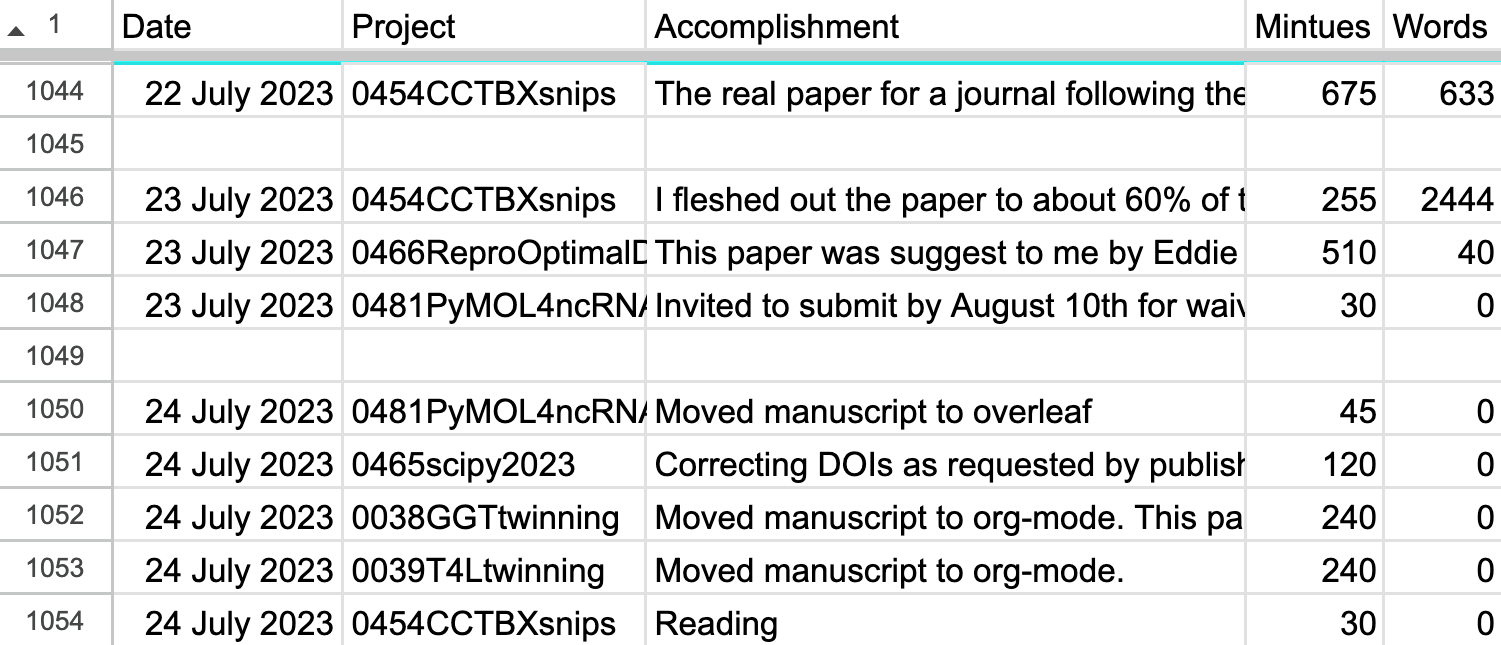
\includegraphics[width=0.94\textwidth, angle=0]{./Figures/OUHSCwritingLog}
\end{center}
\normalsize{Boice,R. (1989) Procrastination, busyness and bingeing. \emph{Behaviour Research and Therapy}, 27, 605–611.}
\end{frame}
\note{ 
I will get to the primary purposes of this running log in a minute but it is not the same as the writing box you May have heard of that are used as an accountability tool.
Here is an example of such an accountability tool in a Google sheet.
By date we have the project and a list of accomplishments as well as minutes spent and words generated.
You can see that on July 24th of 2023 I was able to work on five different writing projects.
I was able to do this because I start every session on a writing project in the writing log in the diary section where I reboot my memory of where I left off so my switching costs are actually very low.
As a result I was able to work on five different projects in a single day.
This is not a typical day for me but example of what is possible using my Project Specific writing log.
In other words I actually made entries in five different writing logs on this particular day about what I did in each of those projects.
And some projects I work for 4 hours and on others I worked for as little as 30 minutes but nonetheless I made progress on five different projects.

This accountability tool looks like extra work but Robert Boyce showed in a systematic study that those academics who keep a record of their writing progress like the one above are four times more productive than academics who did not keep such a writing log.
He then found that those academics who share their writing log with other academics are nine times more productive than those who do not share do not keep a writing log.
This demonstrates the power of this kind of accountability tool.
And in fact the above accountability tool was accessible to three other college of mine they maintain their own writing progress worksheets in this workbook.
The knowledge that they could check up on me had by opening up my worksheet I will stop a lot of progress.
}

\subsection{Number of projects worked per day in 2024}
\begin{frame}
\frametitle{Number of articles worked per day in 2024}
\begin{center}
    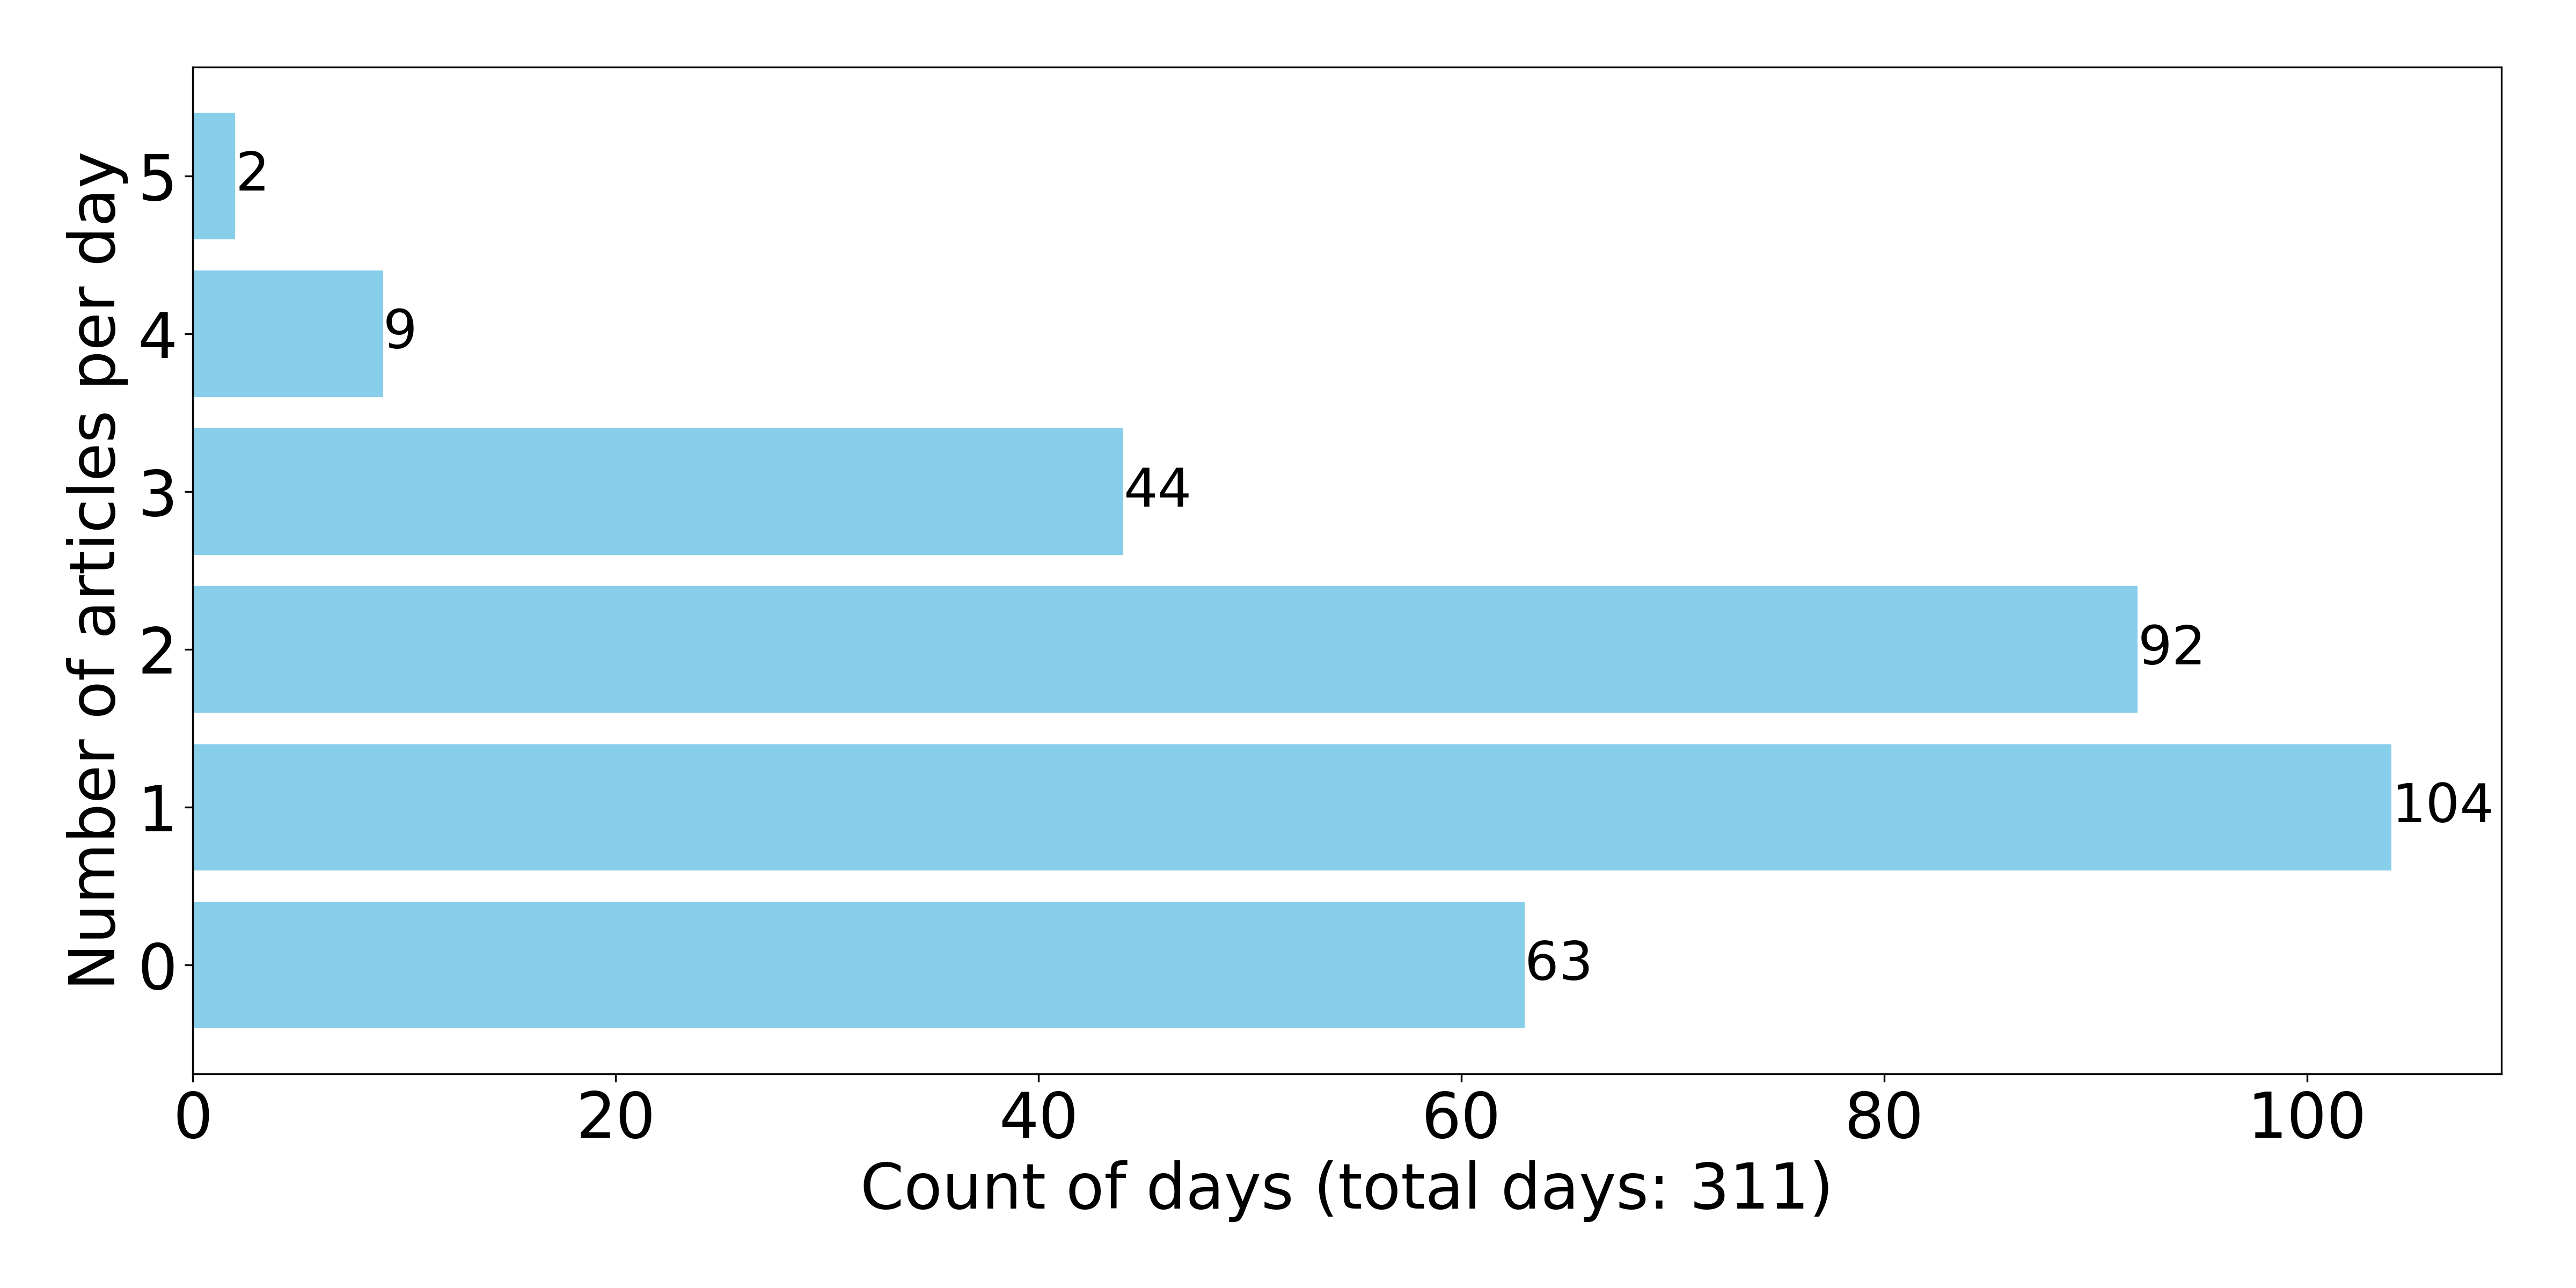
\includegraphics[width=0.9\textwidth, angle=0]{./Figures/pfMarkedHbar}
\end{center}
Worked on 2 or more articles per day 58\% of the days when some journal article writing was done.
\end{frame}
\note{ }


\subsubsection{Motivation for using writing-project log}
\begin{frame}
\frametitle{Motivation behind the writing-project log}
\large{
\textbf{Primary purpose:} support clear thinking to
\begin{itemize}[font=$\bullet$\scshape\bfseries]
   \item improve project's impact (i.e., do better science).
   \item accelerate project completion
\end{itemize}

\textbf{Secondary purpose:} enable work on multiple projects
\begin{itemize}[font=$\bullet$\scshape\bfseries]
   \item ease switching between projects
   \item feed subconscious background jobs
\end{itemize}

\textbf{Side-effects:} peace of mind
\begin{itemize}[font=$\bullet$\scshape\bfseries]
    \item reduced Fear of Forgetting (FoF).
    \item reduced Fear of Losing Momentum (FoLM).
\end{itemize}
\vspace{1em}
\normalsize{Sword, H. (2016) ‘Write every day!’: A mantra dismantled. International Journal for Academic Development, 21, 312–322.}
}
\end{frame}
\note{ 
This writing log addresses a problem of working on more than one writing project at a time. 
Doing so is challenging because of the fears of forgetting and the fears of losing momentum.
Most of the above writing books actually do not address an issue of working on multiple projects in parallel.
This is actually a very hard problem but I think that my approach has some merit.
Just actually more important to spread out effort on a writing project over a long. Of time than to do the preferred approach of just remaining focus on one thing.
Part of the reason for that is that you need to give your subconscious sufficient time to work in the background on the material that you are writing about. If you take the serial approach then you are not going you are limiting the opportunity of for your subconscious to do this work.

I find that the writing log allows me to store my thinking about the writing project and because there has a space available to do so.
This reduces by fewer forgetting where I left off and my fear of losing momentum.
Also find that making notes about a single project in a single document helps me focus on that one project.
}


\subsubsection{Overview of writing-project log in Org Mode}
\begin{frame}
\frametitle{Overview of writing-project log in Org Mode}
\begin{center}
\begin{figure}
    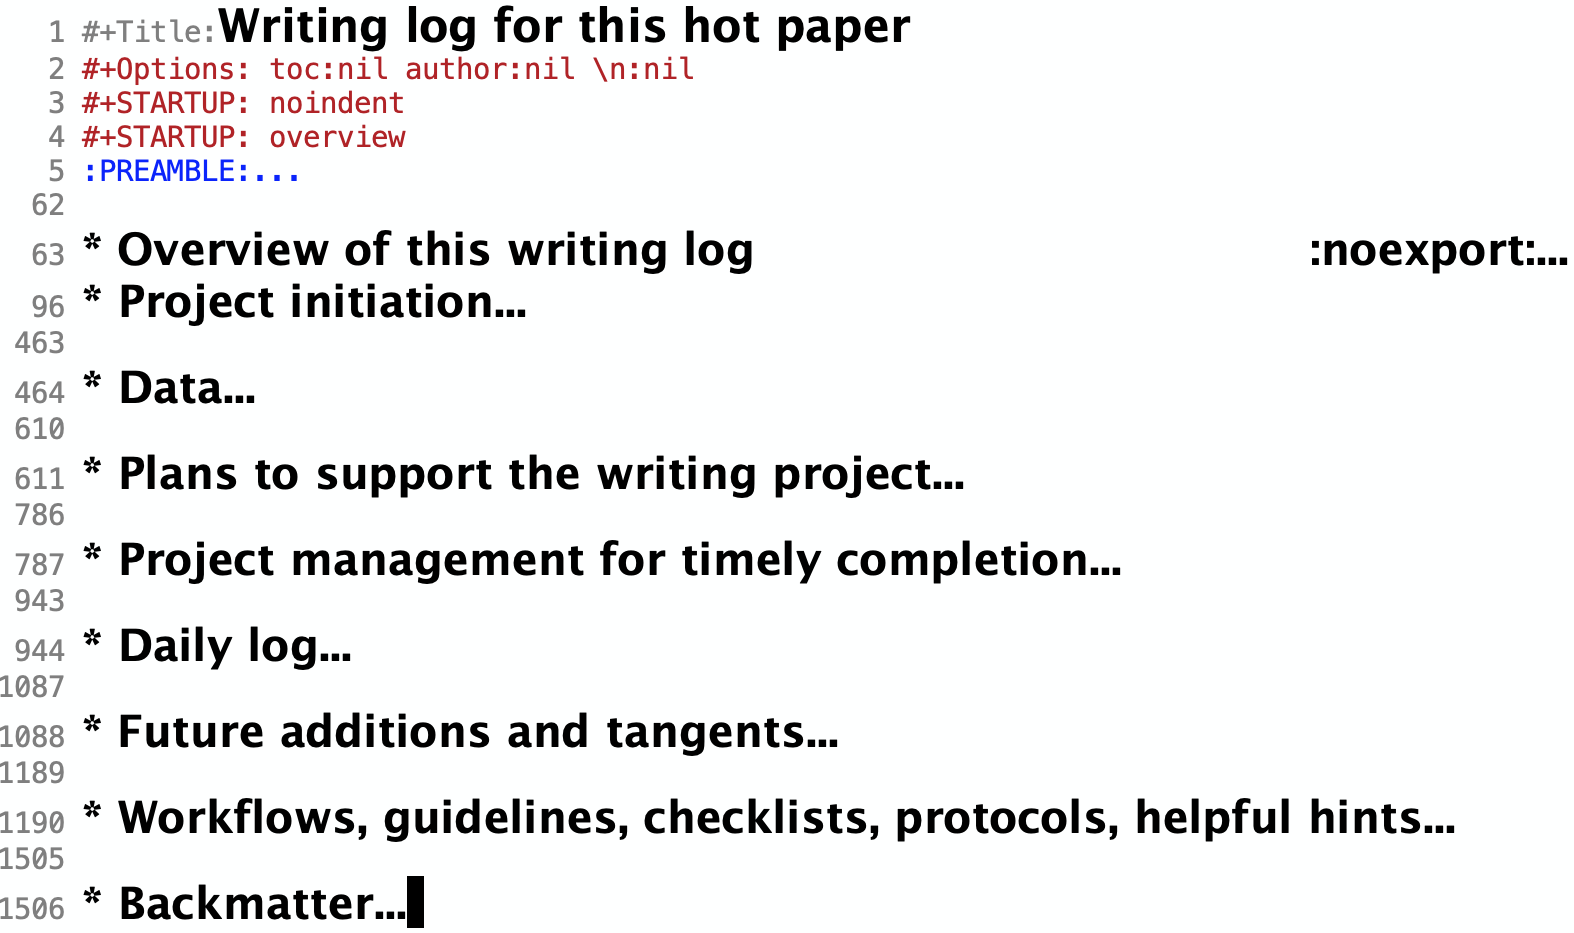
\includegraphics[scale=0.235]{Figures/overview.png}
\end{figure}
\end{center}
\end{frame}


% \subsection{LaTeX Preamble}
% \begin{frame}
% \frametitle{LaTeX preamble in opened drawer}
% \begin{center}
% \begin{figure}
%     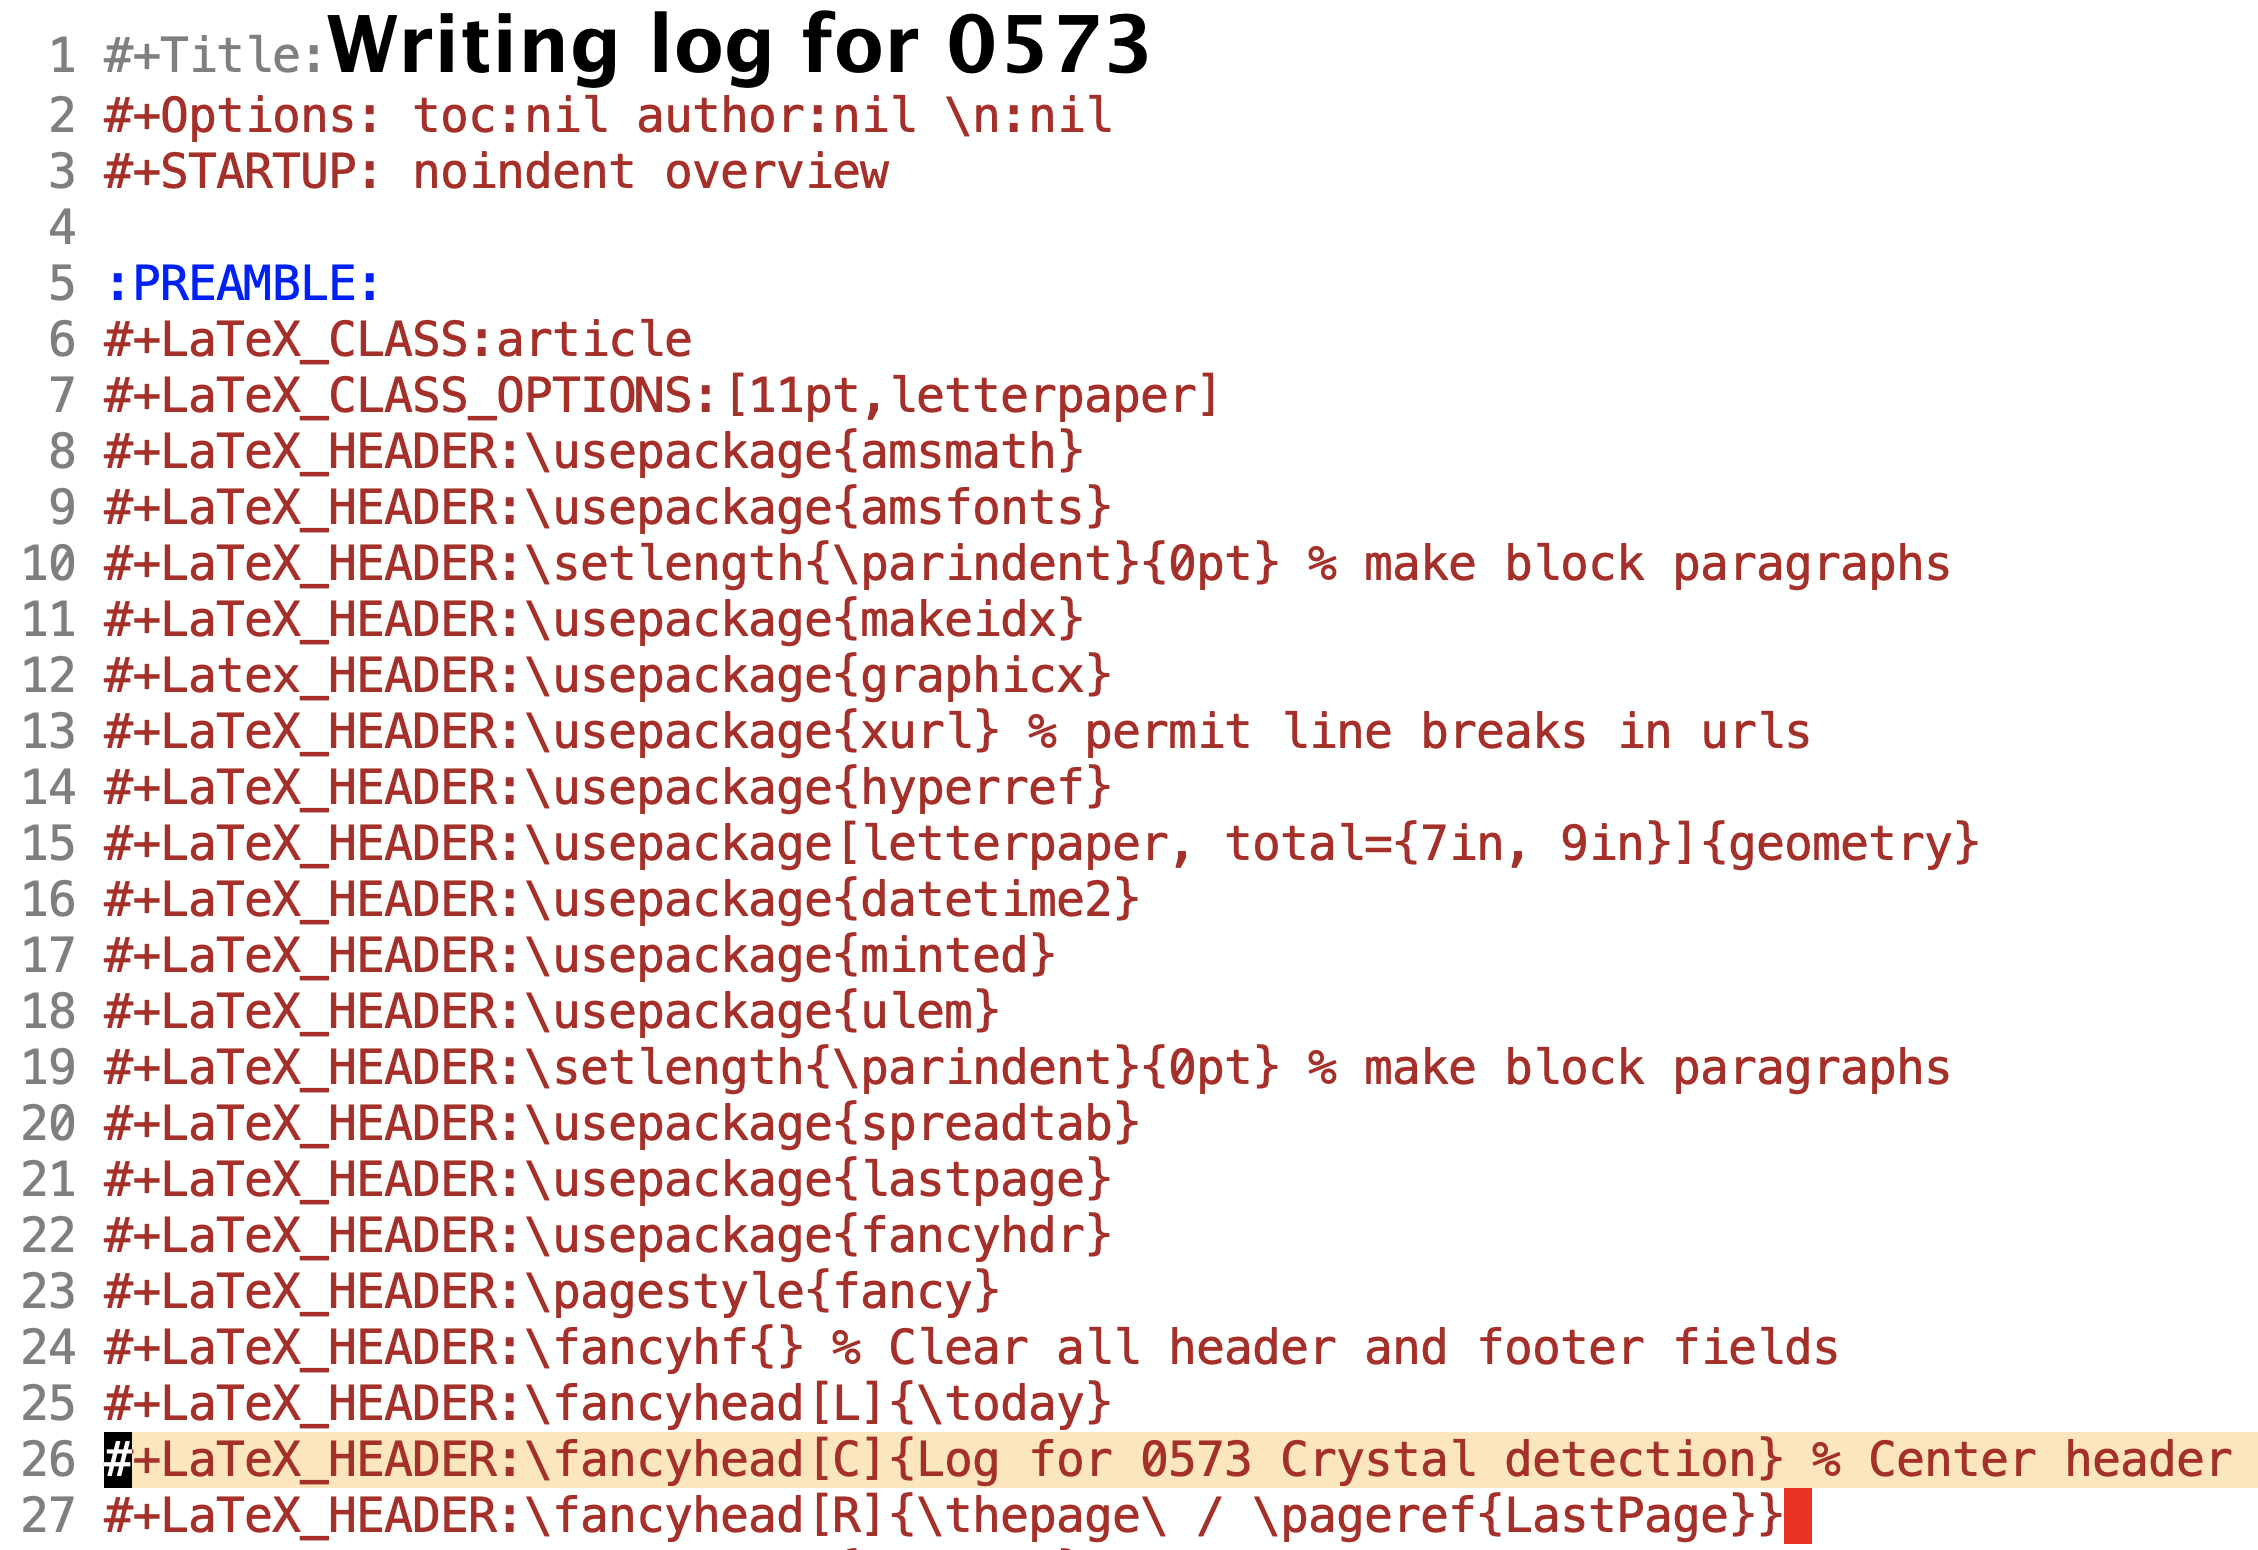
\includegraphics[scale=0.275]{Figures/preamble.png}
% \end{figure}
% \end{center}
% \end{frame}

% \subsection{Header}
% \begin{frame}
% \frametitle{Informative header}
% \begin{center}
% \begin{figure}
%     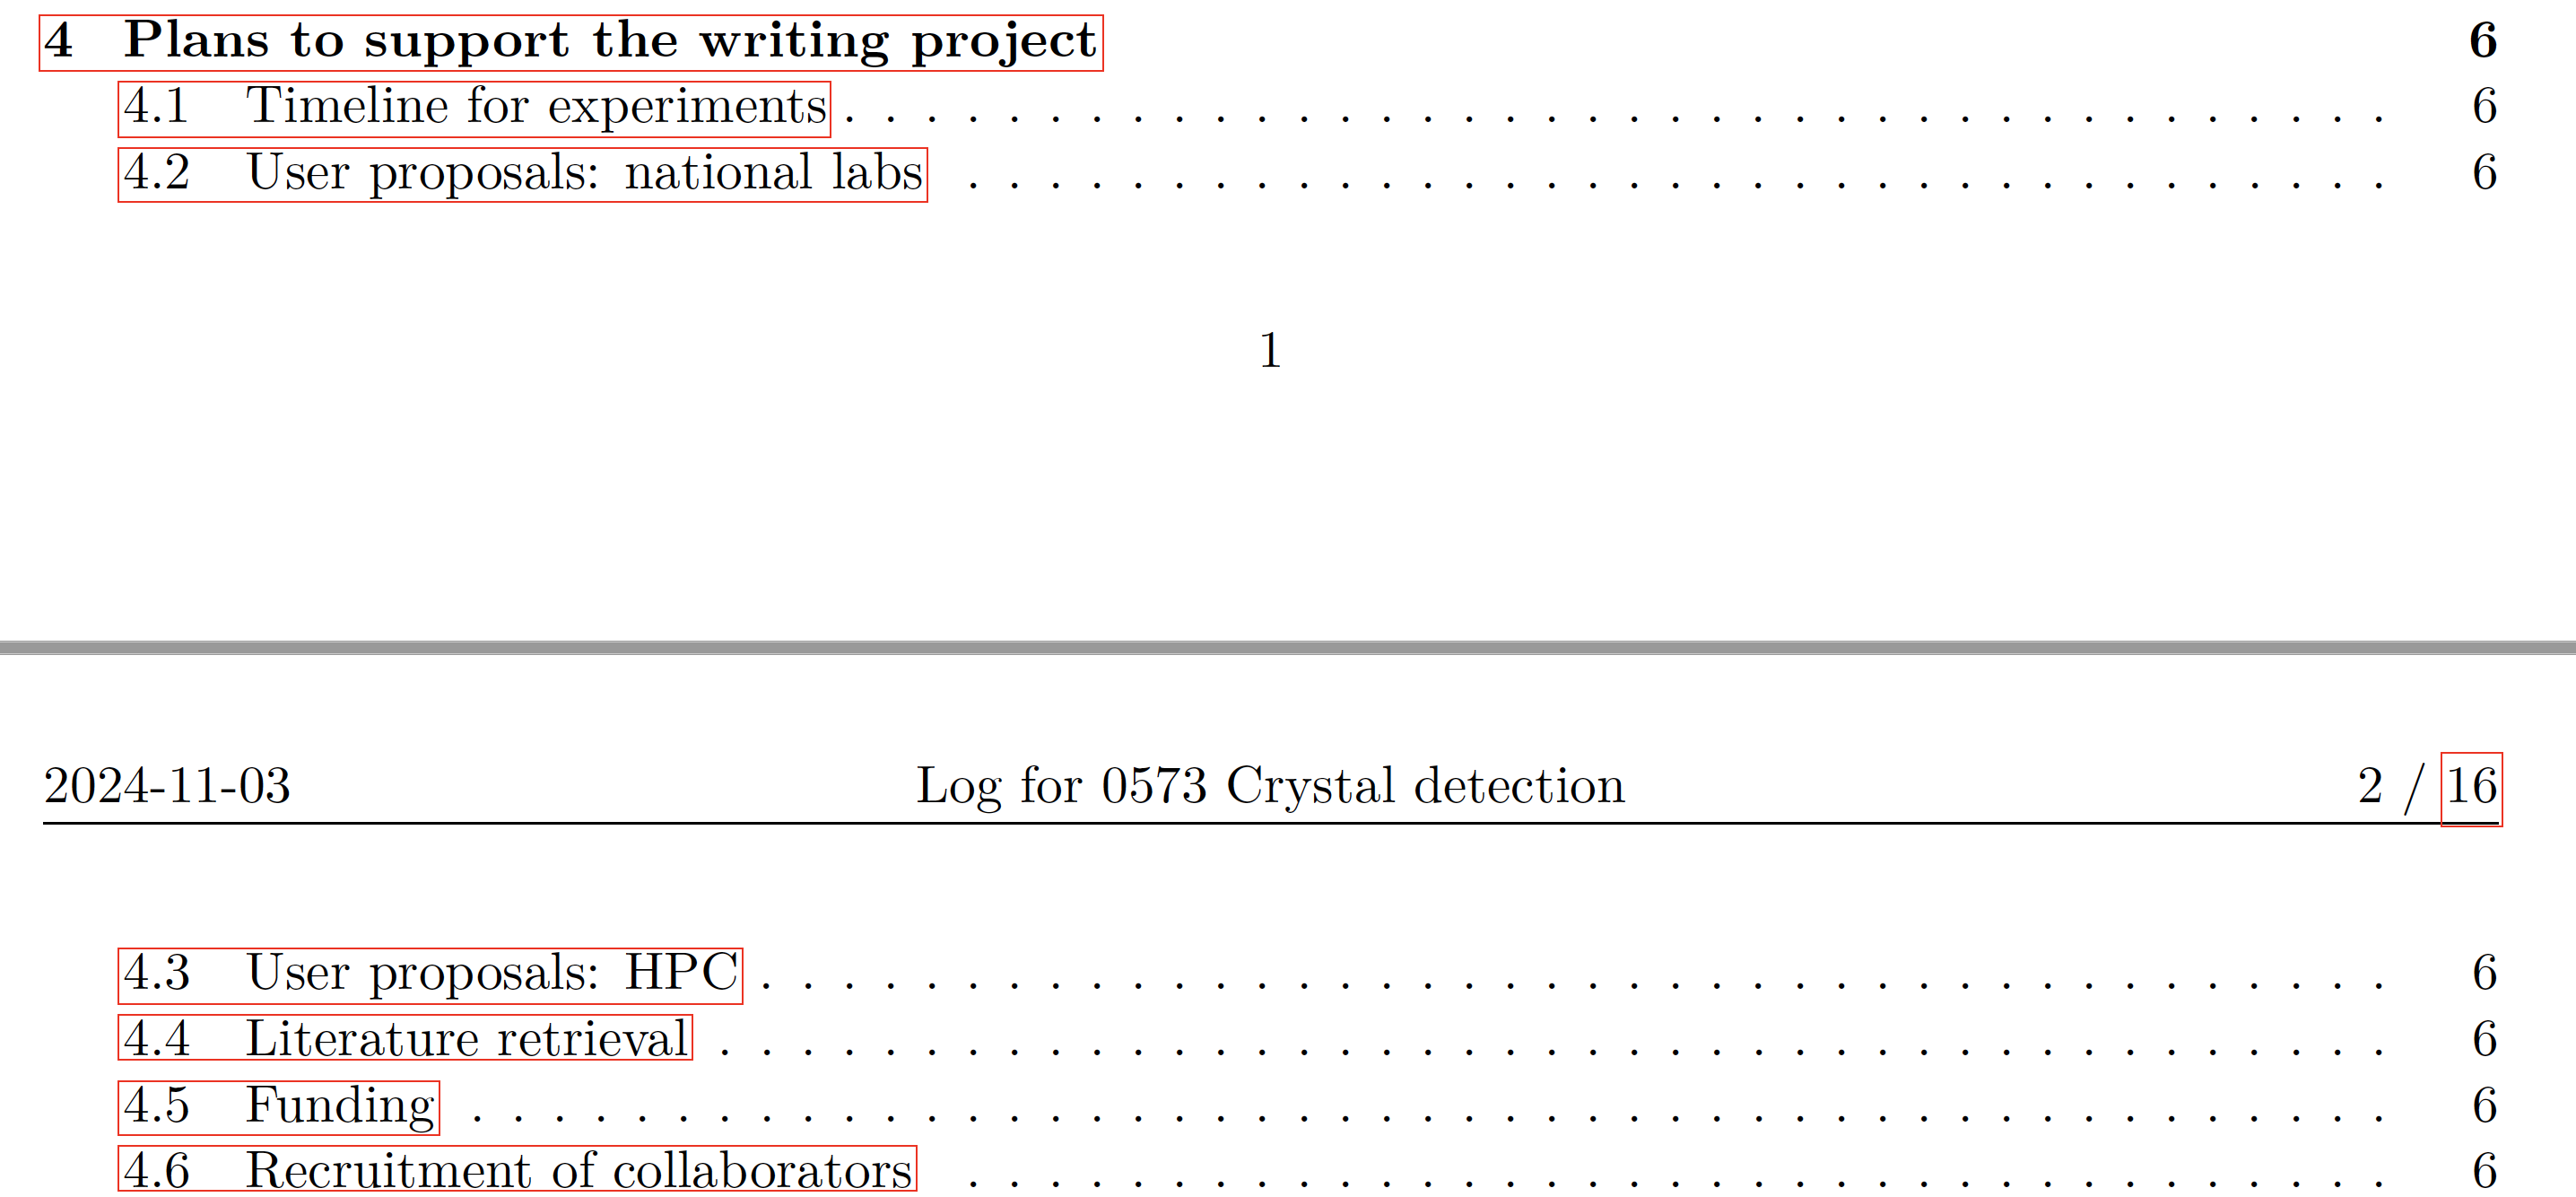
\includegraphics[scale=0.28]{Figures/informativeHeader.png}
% \end{figure}
% \end{center}
% \end{frame}

\subsubsection{Additional features of the template}
\begin{frame}
\frametitle{Additional features of the template}
\Large{
\begin{columns}
    \begin{column}{0.45\textwidth}

        \begin{itemize}[font=$\bullet$\scshape\bfseries]
            \item Table of contents
            \item Images
            \item Tables
            \item Equations
            \item Code blocks
        \end{itemize}
    \end{column}
    \begin{column}{0.45\textwidth}
        \begin{itemize}[font=$\bullet$\scshape\bfseries]
            \item Index
            \item List of acronyms
            \item Glossary
            \item Mathematical notation
            \item Literature Cited
        \end{itemize}
    \end{column}
    \end{columns}
    \vspace{2em}
    These features are also available in the annotated bibliography template.
    }
\end{frame}
\note{
https://app.leonardo.ai/image-generation
}



\subsubsection{Four workflows in Log File}
\begin{frame}
\frametitle{Four workflows}
    \begin{columns}
        \begin{column}{0.55\textwidth}
\Large{
\begin{itemize}[font=$\bullet$\scshape\bfseries]
    \item Project initiation 
    \item Daily 
    \item Periodic assessment
    \item Project closeout 
\end{itemize}
}
        \end{column}
        \begin{column}{0.45\textwidth}
            \begin{figure}
                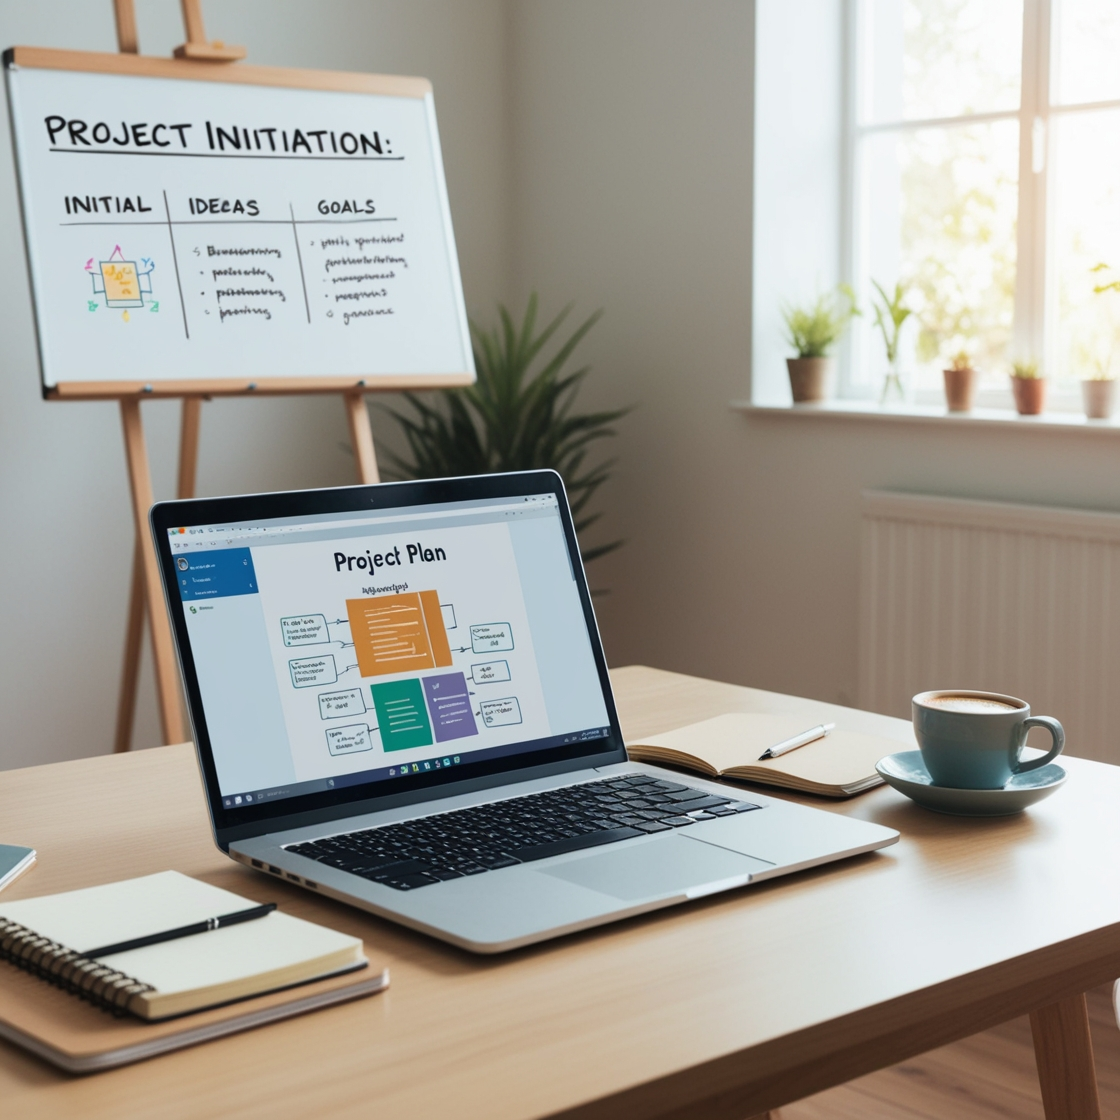
\includegraphics[width=\textwidth]{Figures/ProjectInitiationOld.jpg}
            \end{figure}
        \end{column}
    \end{columns}
\end{frame}
\note{
https://app.leonardo.ai/image-generation
}


\subsubsection{Initiation in org}
\begin{frame}
\frametitle{Project initiation workflow}
\begin{center}
            \begin{figure}
                
\includegraphics[scale=0.235]{Figures/targetJournals0573.png}
            \end{figure}
\end{center}
\end{frame}
\note{ 
Guidance of
}



% \subsection{Ideation part 1}
% \begin{frame}
% \begin{center}
%             \begin{figure}
%                 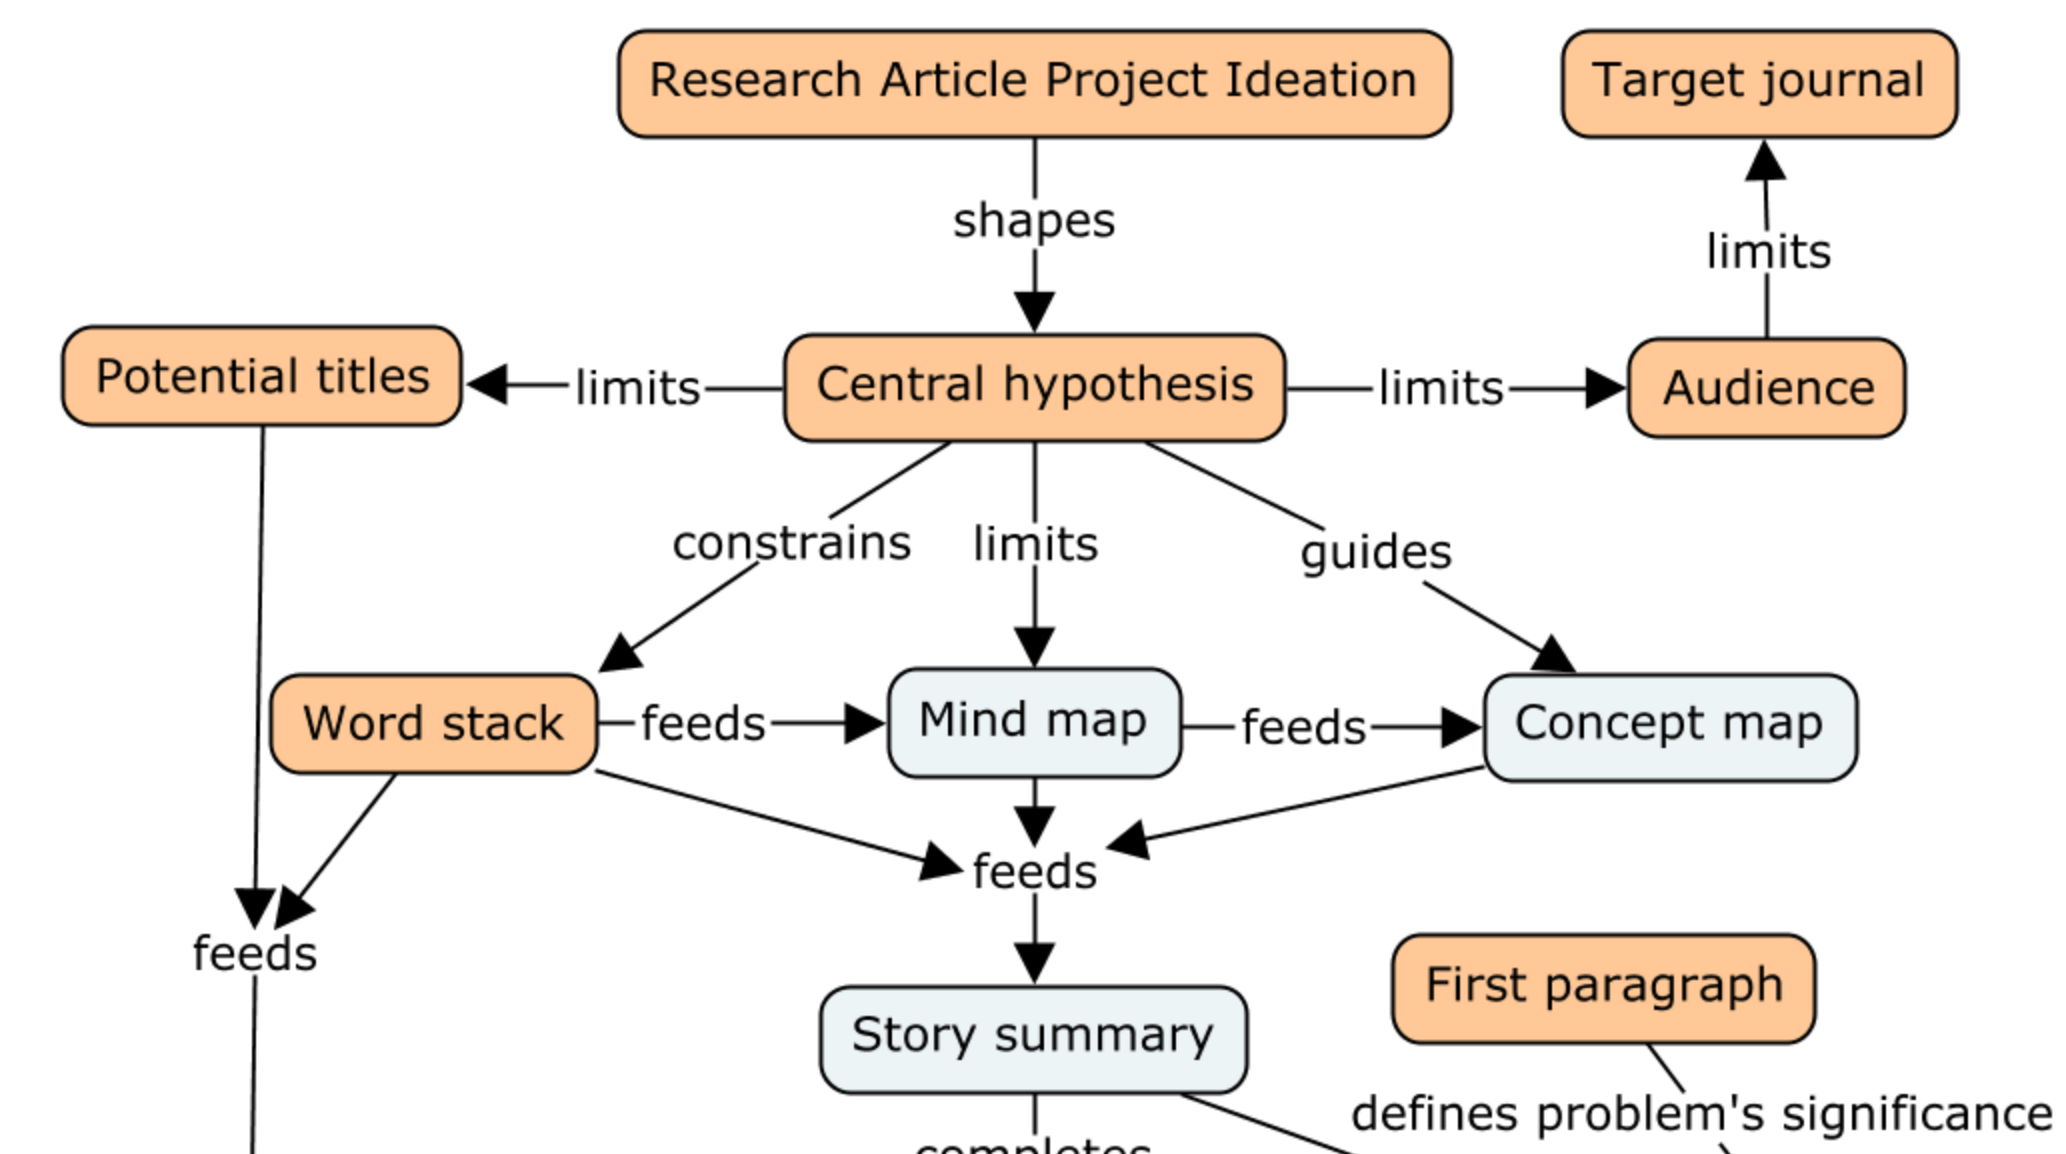
\includegraphics[scale=0.385]{Figures/topHalfIdeation.png}
%             \end{figure}
% \end{center}
% \end{frame}
% \note{ 
% Guidance of
% }


% \subsection{Story Summary}
% \begin{frame}
% \frametitle{Nine questions driving story summary}
% \begin{center}
%             \begin{figure}
%                 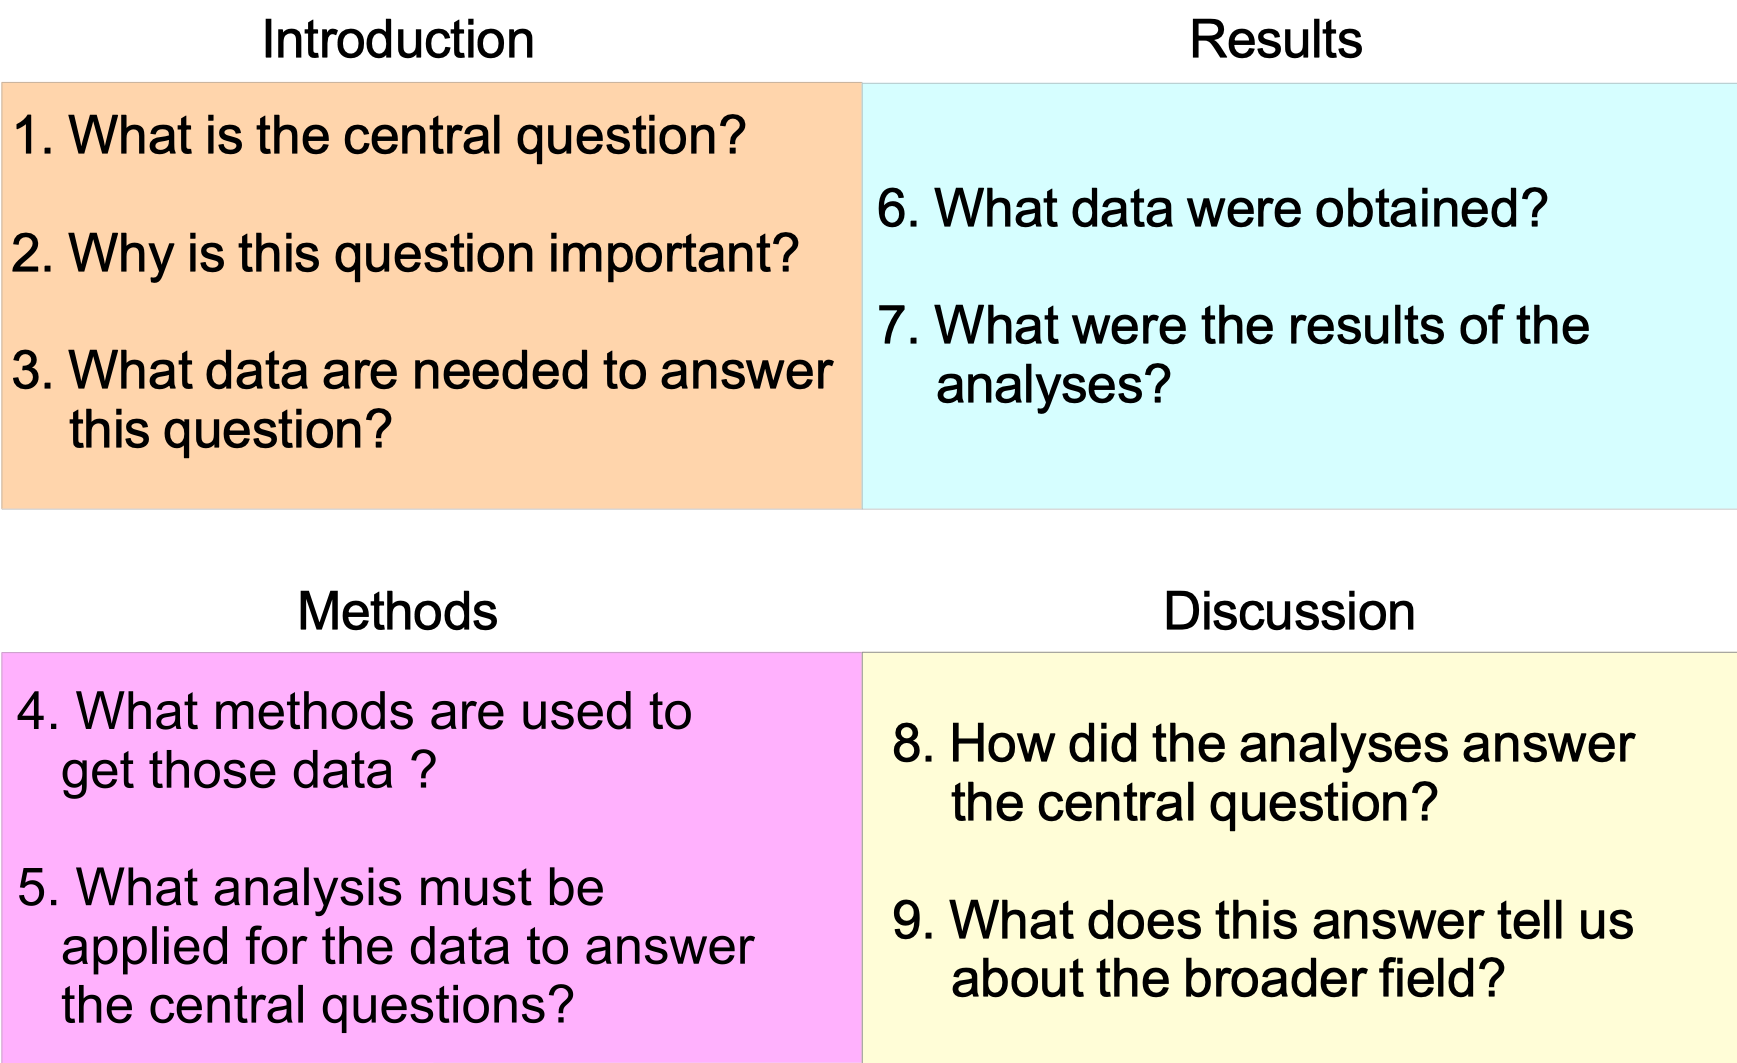
\includegraphics[scale=0.16]{Figures/StorySummary2.png}
%             \end{figure}
% \end{center}
% \footnotesize{Heard, S.B. (2022) The scientist’s guide to writing: how to write more easily and effectively throughout your scientific career 2nd ed. Princeton University Press.}
% \end{frame}
% \note{ }


% \subsection{Ideation part 2}
% \begin{frame}
% \begin{center}
%             \begin{figure}
%                 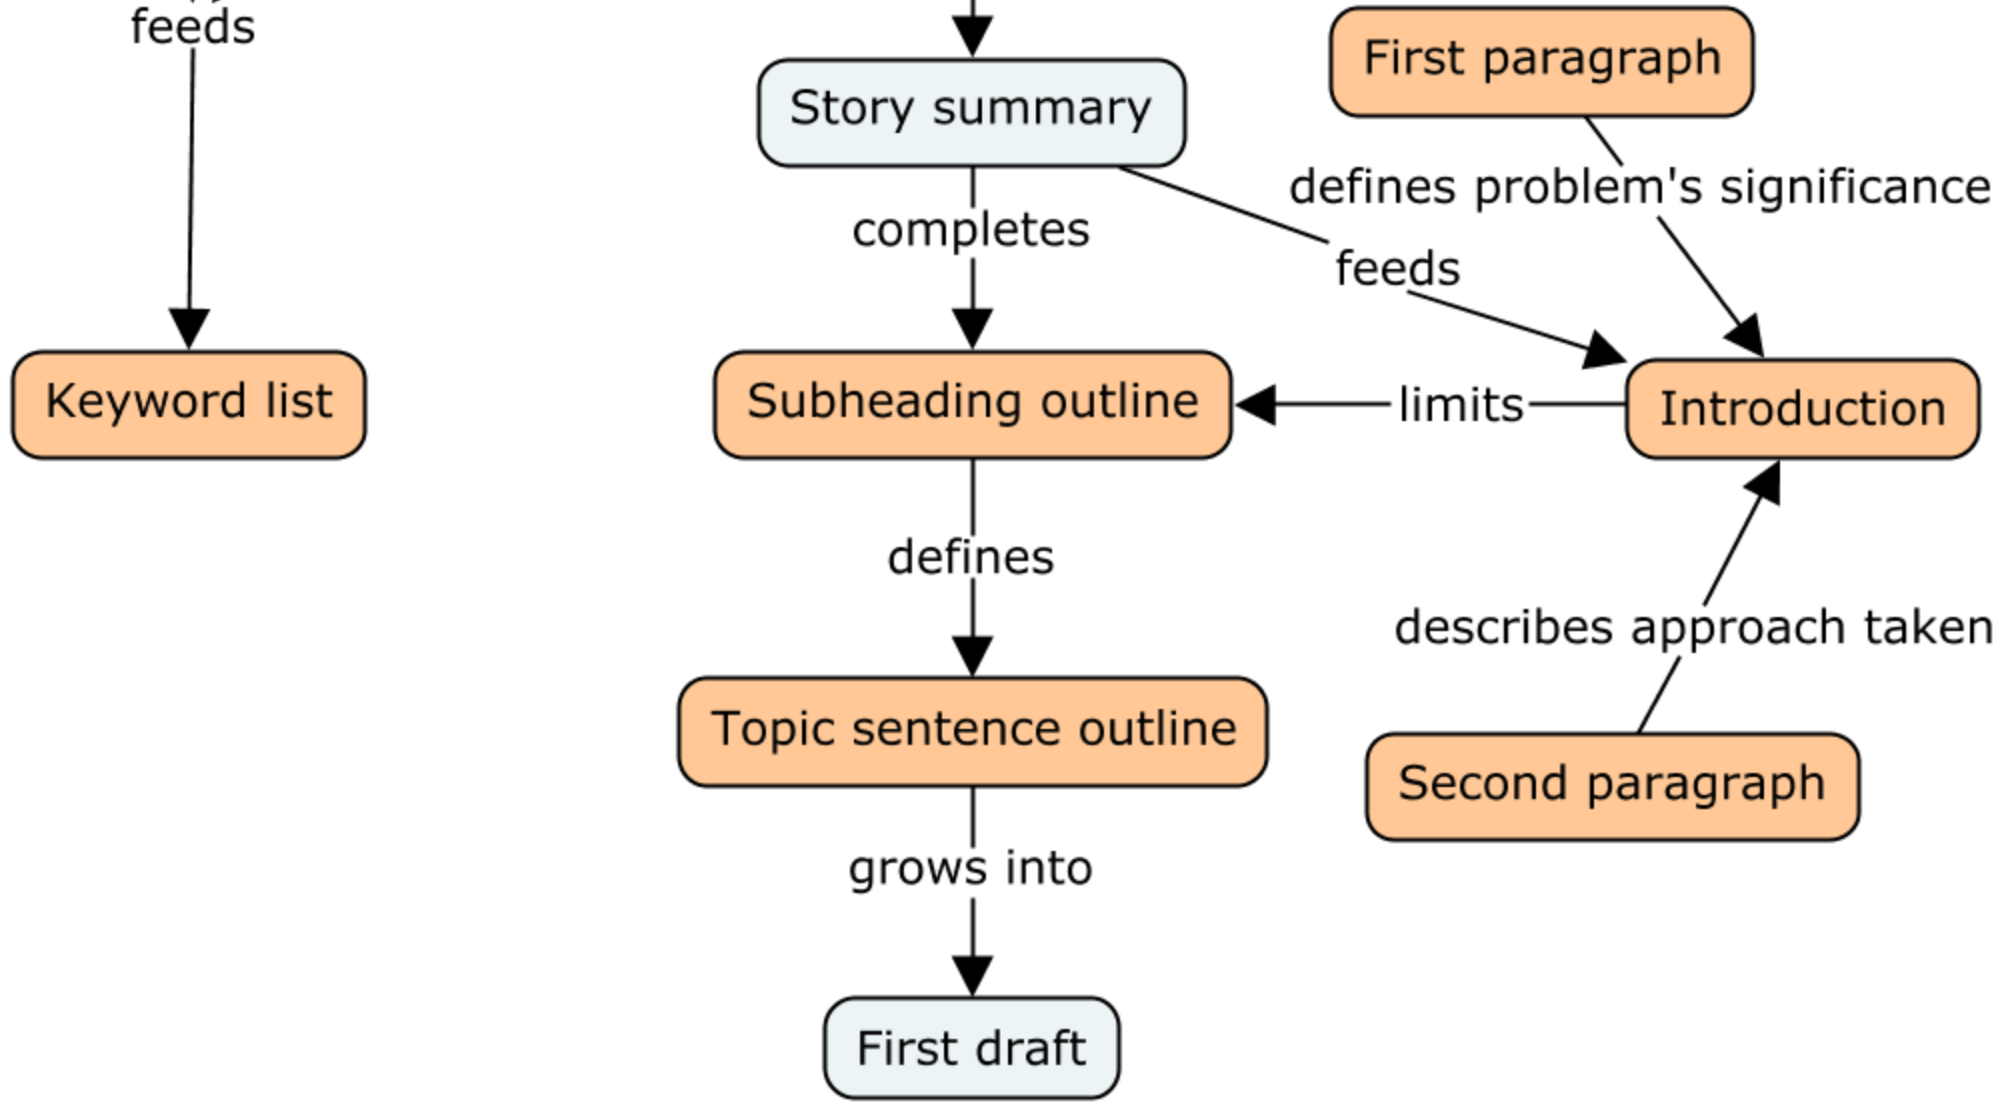
\includegraphics[scale=0.385]{Figures/bottomHalfIdeation.png}
%             \end{figure}
% \end{center}
% \end{frame}
% \note{ }


% \subsection{Daily workflow}
% \begin{frame}
% \frametitle{Daily workflow [?]}
% \Large{
% \begin{itemize}
% \item 1. Review timeline, recent entries, next action, to-dos.
% \item 2. [Optional] Enter goal(s) for the current writing session.
% \item 3. At end of session, add finished tasks to accomplishments list.
% \item 4. Insert correspondences, decisions made, and metadata.
% \item 5. Move unfinished tasks to to-dos.
% \item 6. [Optional] Select one task for next action.
% \end{itemize}
% }
% \end{frame}
% \note{
% I might be able to describe this verbally without this list of 
% }

\subsubsection{Daily Entry Example}
\begin{frame}
\frametitle{Daily workflow}
\begin{figure}
    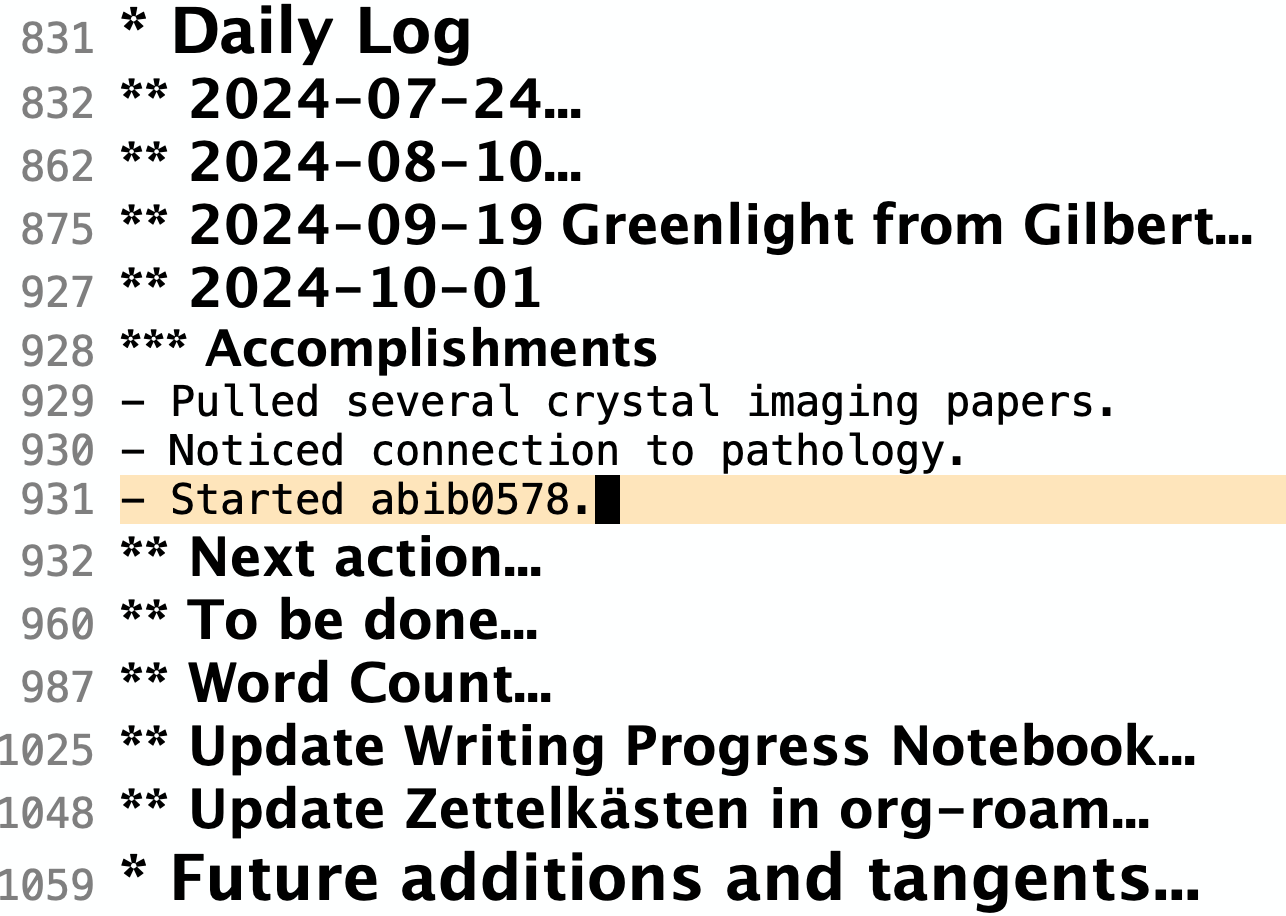
\includegraphics[scale=0.23]{Figures/DailyLog0578}
\end{figure}
\end{frame}
\note{
Here is an example of a daily entry.
I enter these sequentially.
I wrote a yasnippet snippet that starts the entry with the current date.
I might write a few goals that I want to accomplish after reviewing the prior entry and my to-do list.
If I was strictly following the Jim Allen's protocol I would use the started on the next but often I find that I change my mind as to what I should work on next between writing sessions.
I have an external like a to-do list that I keep for the day that where I will assemble my planned actions and then I will transfer them this writing log.
It do not really matter how you do it or if you can enter any goals.
Then I go off and do the work and when I come back I will enter a list of what was accomplished.
If I had some correspondence I will also Pace that in a quote block.
I will also record any my decisions at a wrestled with and and the rationale is to behind the choice that I made.
If the past had a pick was too large then to finish then I will move it to the next.
I will update my to-do list with any new tasks that I thought of.
Sometimes in the course of the tangential idea that is not something that I would ruin necessarily do right now with regard to this project but that could be done as part of some future paper so I will store that in a sort of future ideas section.
I realize that some people would take a similar approach but this is more focused and I do not have to worry about using filters to find my stuff again.
At the end of the work session they also update today workout file from tracking word count and I am also update any done
}

\subsubsection{Periodic assessment workflow}
\begin{frame}
\frametitle{Periodic assessment workflow}
\begin{figure}
    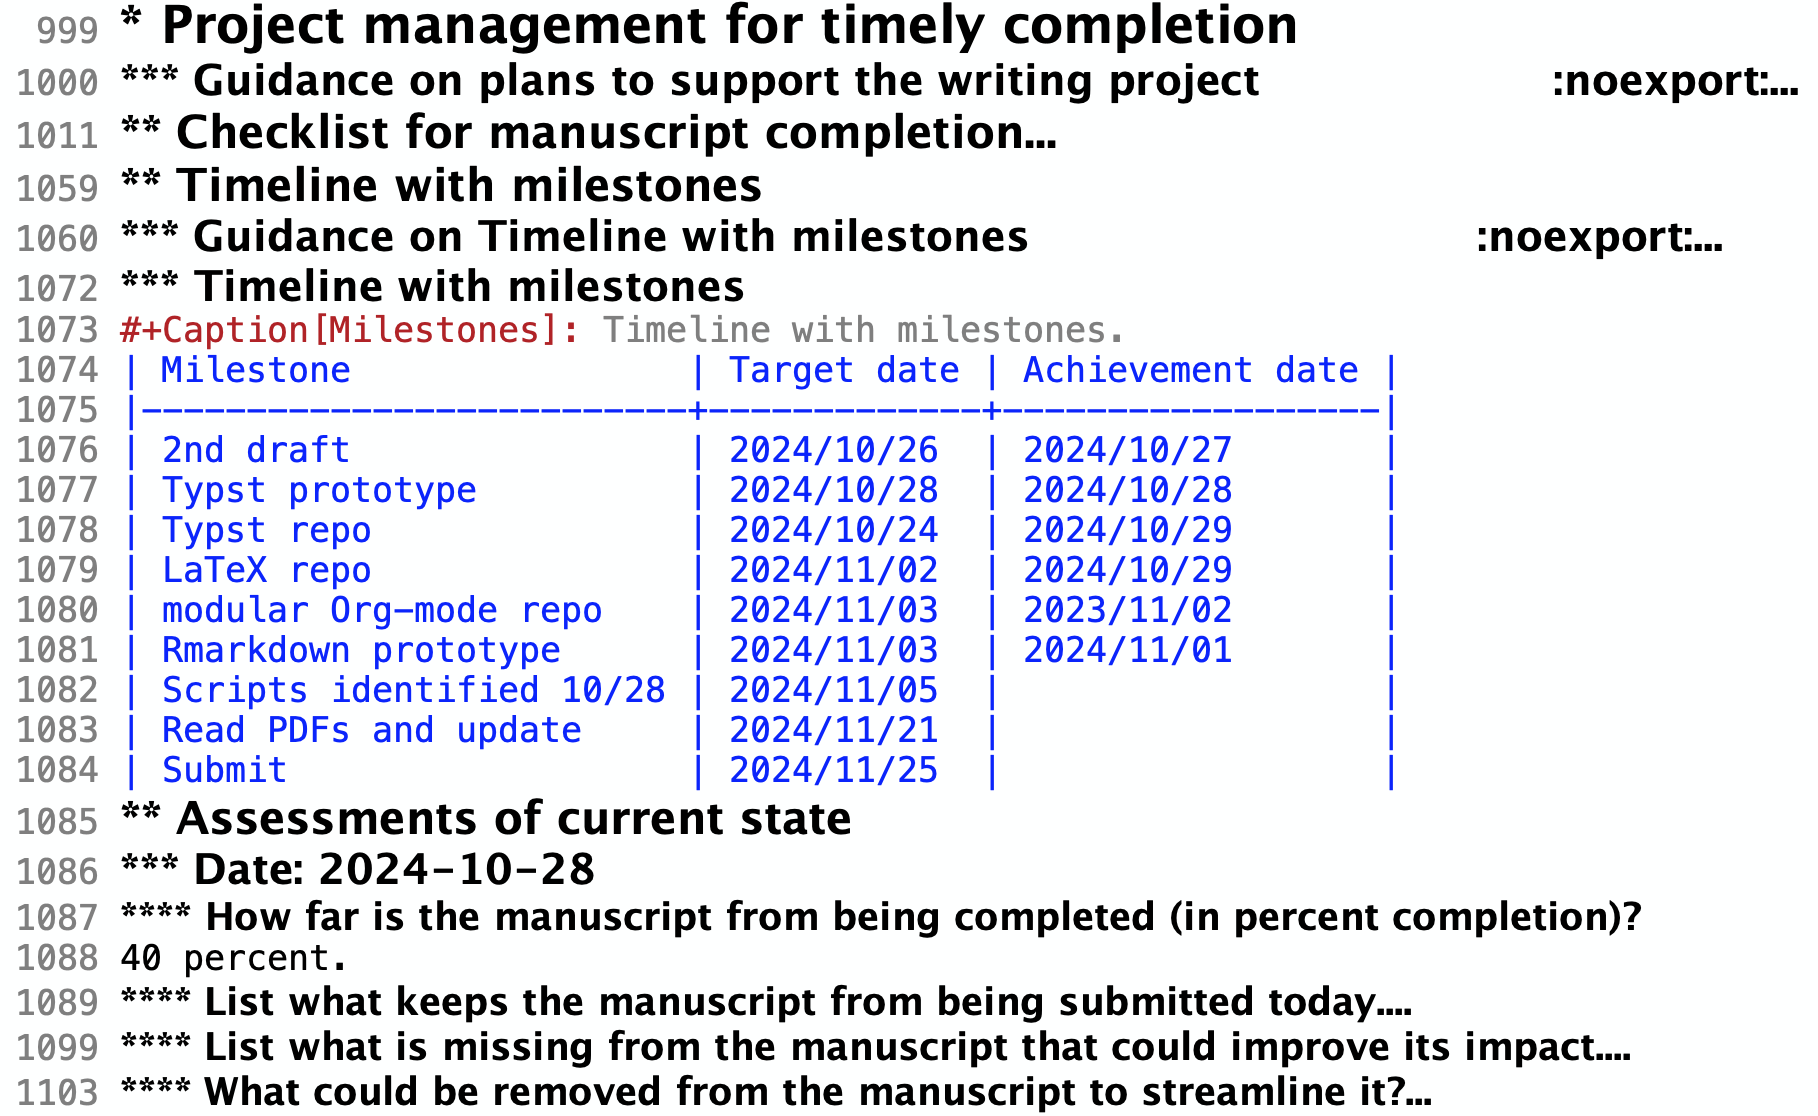
\includegraphics[scale=0.18]{Figures/periodicAssessment}
\end{figure}
\end{frame}


\subsubsection{Project closeout workflow}
\begin{frame}
\frametitle{Project closeout workflow}
\begin{figure}
    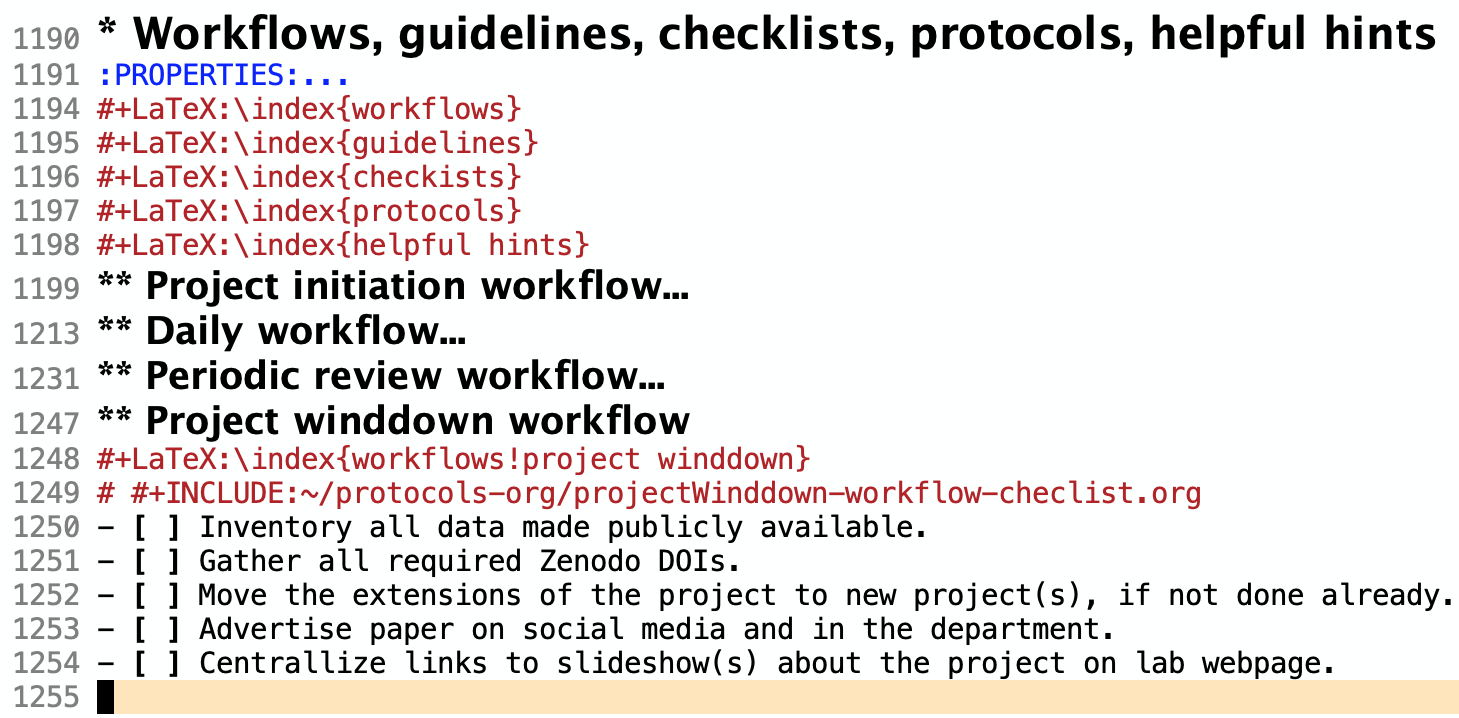
\includegraphics[scale=0.27]{Figures/projectWinddownWorkflow.png}
\end{figure}
\end{frame}



\subsection{Conclusions}
\begin{frame}
\frametitle{Conclusions}
\Large{
\begin{itemize}[font=$\bullet$\scshape\bfseries]
    \item Project-specific log file narrows the focus to one project.
    \item Log harbors thinking about the writing project. 
    \item Log supports project initiation, momentum, and completion.
    \item Side effects: dampened FoF and FoLM, which reduce barriers to working on multiple projects in one day.
\end{itemize}
}
\end{frame}

% \section{Paths not taken}
% \begin{frame}
% \frametitle{Alternate approaches}
% \Large{
% \begin{itemize}[font=$\bullet$\scshape\bfseries]
%     \item Org-roam (+ reduce redundant effort, retrieve with tags) (- not sharable, no support for collaboration)
%     \item personal LLM (+ easy, - incomplete retrieval, - not collaborative)
%     \item Integrate with org-agenda
%     \item 
%     \item 
% \end{itemize}
% }
% \end{frame}




\subsection{Acknowledgements}
\begin{frame}
\frametitle{Acknowledgements}
\Large{
Friends and mentors:
\begin{itemize}[font=$\bullet$\scshape\bfseries]
\item Oklahoma Data Science Workshop
\item Berlin and Austin Emacs Meetups
\item Vidianos Giannitsis, David Pérez-Suárez, and the UK-RSE M-x research Slack Channel
\end{itemize}
\vspace{0.5cm}
Support for working in Emacs all day:
\begin{itemize}[font=$\bullet$\scshape\bfseries]
    \item NIH: R01 CA242845, R01 AI088011
    \item NIH: P30 GM145423, P30 CA225520, P30 AG050911-07S1 
    \item OCAST HR20-002
\end{itemize}
}
\end{frame}
\note{
I would like to thank feedback on this project from our local Data Science Workshop that meets once a month.
I would also like to thank these funding sources that supported this work.
}

% *********************************************** Overflow **************************************************

\subsubsection{Other potential logs}
\begin{frame}
\frametitle{Other potential logs}
\begin{columns}
    \begin{column}{0.28\textwidth}
       \large{\textbf{Scholarship:}}
        \begin{itemize}[font=$\bullet$\scshape\bfseries]
            \item journal article
            \item grant application
            \item conference paper
            \item book chapter
            \item book
            \item talk
            \item seminar
            \item poster
            \item patents
        \end{itemize}
    \end{column}
    
    \begin{column}{0.42\textwidth}
      \large{\textbf{Teaching:}}
        \begin{itemize}[font=$\bullet$\scshape\bfseries]
            \item didactic teaching
            \item recruitment
            \item mentoring
          \begin{itemize}[font=$\rightarrow$\scshape\bfseries]
            \item junior faculty, staff scientists
            \item postdoc, technicians
            \item graduate student
            \item exam committee
            \item thesis committee
            \item rotation student
            \item summer student
            \item undergraduate student
            \item high school student
          \end{itemize}
        \end{itemize}
    \end{column}
    
    \begin{column}{0.3\textwidth}
    \large{\textbf{Service:}}
        \begin{itemize}[font=$\bullet$\scshape\bfseries]
            \item manuscript reviewer
            \item special issue editor
            \item associate editor
            \item journal editor
            \item workshop chair
            \item meeting organizer
            \item committee chair
            \item grant reviewer
            \item core lab director
        \end{itemize}
    \end{column}
\end{columns}
\end{frame}
\note{
I have discussed the use of a project log designed to assist with the writing of scientific journal articles.
This template can be adapted to many other kinds of projects.
I have listed the universal three categories of activities that academics are evaluated on every year: scholarship, teaching, and service.
For some of these activities, the log would have different checklists and protocols.

All these logs would have in common a central diary section for recording the daily accomplishments, decision, and correspondence.
The development of these checklists stored in template documents can greatly help one take in a more systematic approach to these activities and thereby helping one be more effective and efficient.

The decision as to whether or not to develop a project log for one of these kinds of projects will depend on how much effort you want to sink into the project.
I think that if you are going to have to do these activities of four more times along a timeline in the future, then a project log can help you remember and track your thoughts about such projects.
I plan to develop project log templates for some of these categories in org-mode.
}


% \subsection{Modular annotated bibliography}
% \begin{frame}
% \frametitle{Modular annotated bibliography}
% \end{frame}
% \subsubsection{Overview of main document with bibentry injection}
% \begin{frame}
% \frametitle{Overview of main document with bibentry injection}
% \end{frame}
% \subsubsection{Sample bibnote}
% \begin{frame}
% \frametitle{Sample bibnote}
% \end{frame}
% \subsubsection{Samples list of acronyms, glossary and math notation}
% \begin{frame}
% \frametitle{Samples list of acronyms, glossary and math notation}
% \end{frame}
% \subsubsection{Org-capture of bibnote}
% \begin{frame}
% \frametitle{Org-capture of bibnote}
% \end{frame}
% \subsection{Introduction to org-roam}
% \begin{frame}
% \frametitle{Introduction to org-roam}
% \end{frame}

% \subsubsection{Introduction to zettelkastens}
% \begin{frame}
% \frametitle{Software zettelkastens}
% \Large{
% \begin{itemize}[font=$\bullet$\scshape\bfseries]
% \item Obsidian (free, desktop app, huge community)
% \item Dendron (VSC, abandoned)
% \item Roam (proprietary)
% \item org-roam (community favorite)
% \item denote (minimalistic, by Prot [Protesilaos Stavrou])
% \end{itemize}
% }
% \end{frame}

% \subsubsection{org-capture org-roam}
% \begin{frame}
% \frametitle{org-capture org-roam}
% \end{frame}

\subsubsection{org-roam-ui}
\begin{frame}
\frametitle{Introduction to org-roam-ui}
\begin{center}
    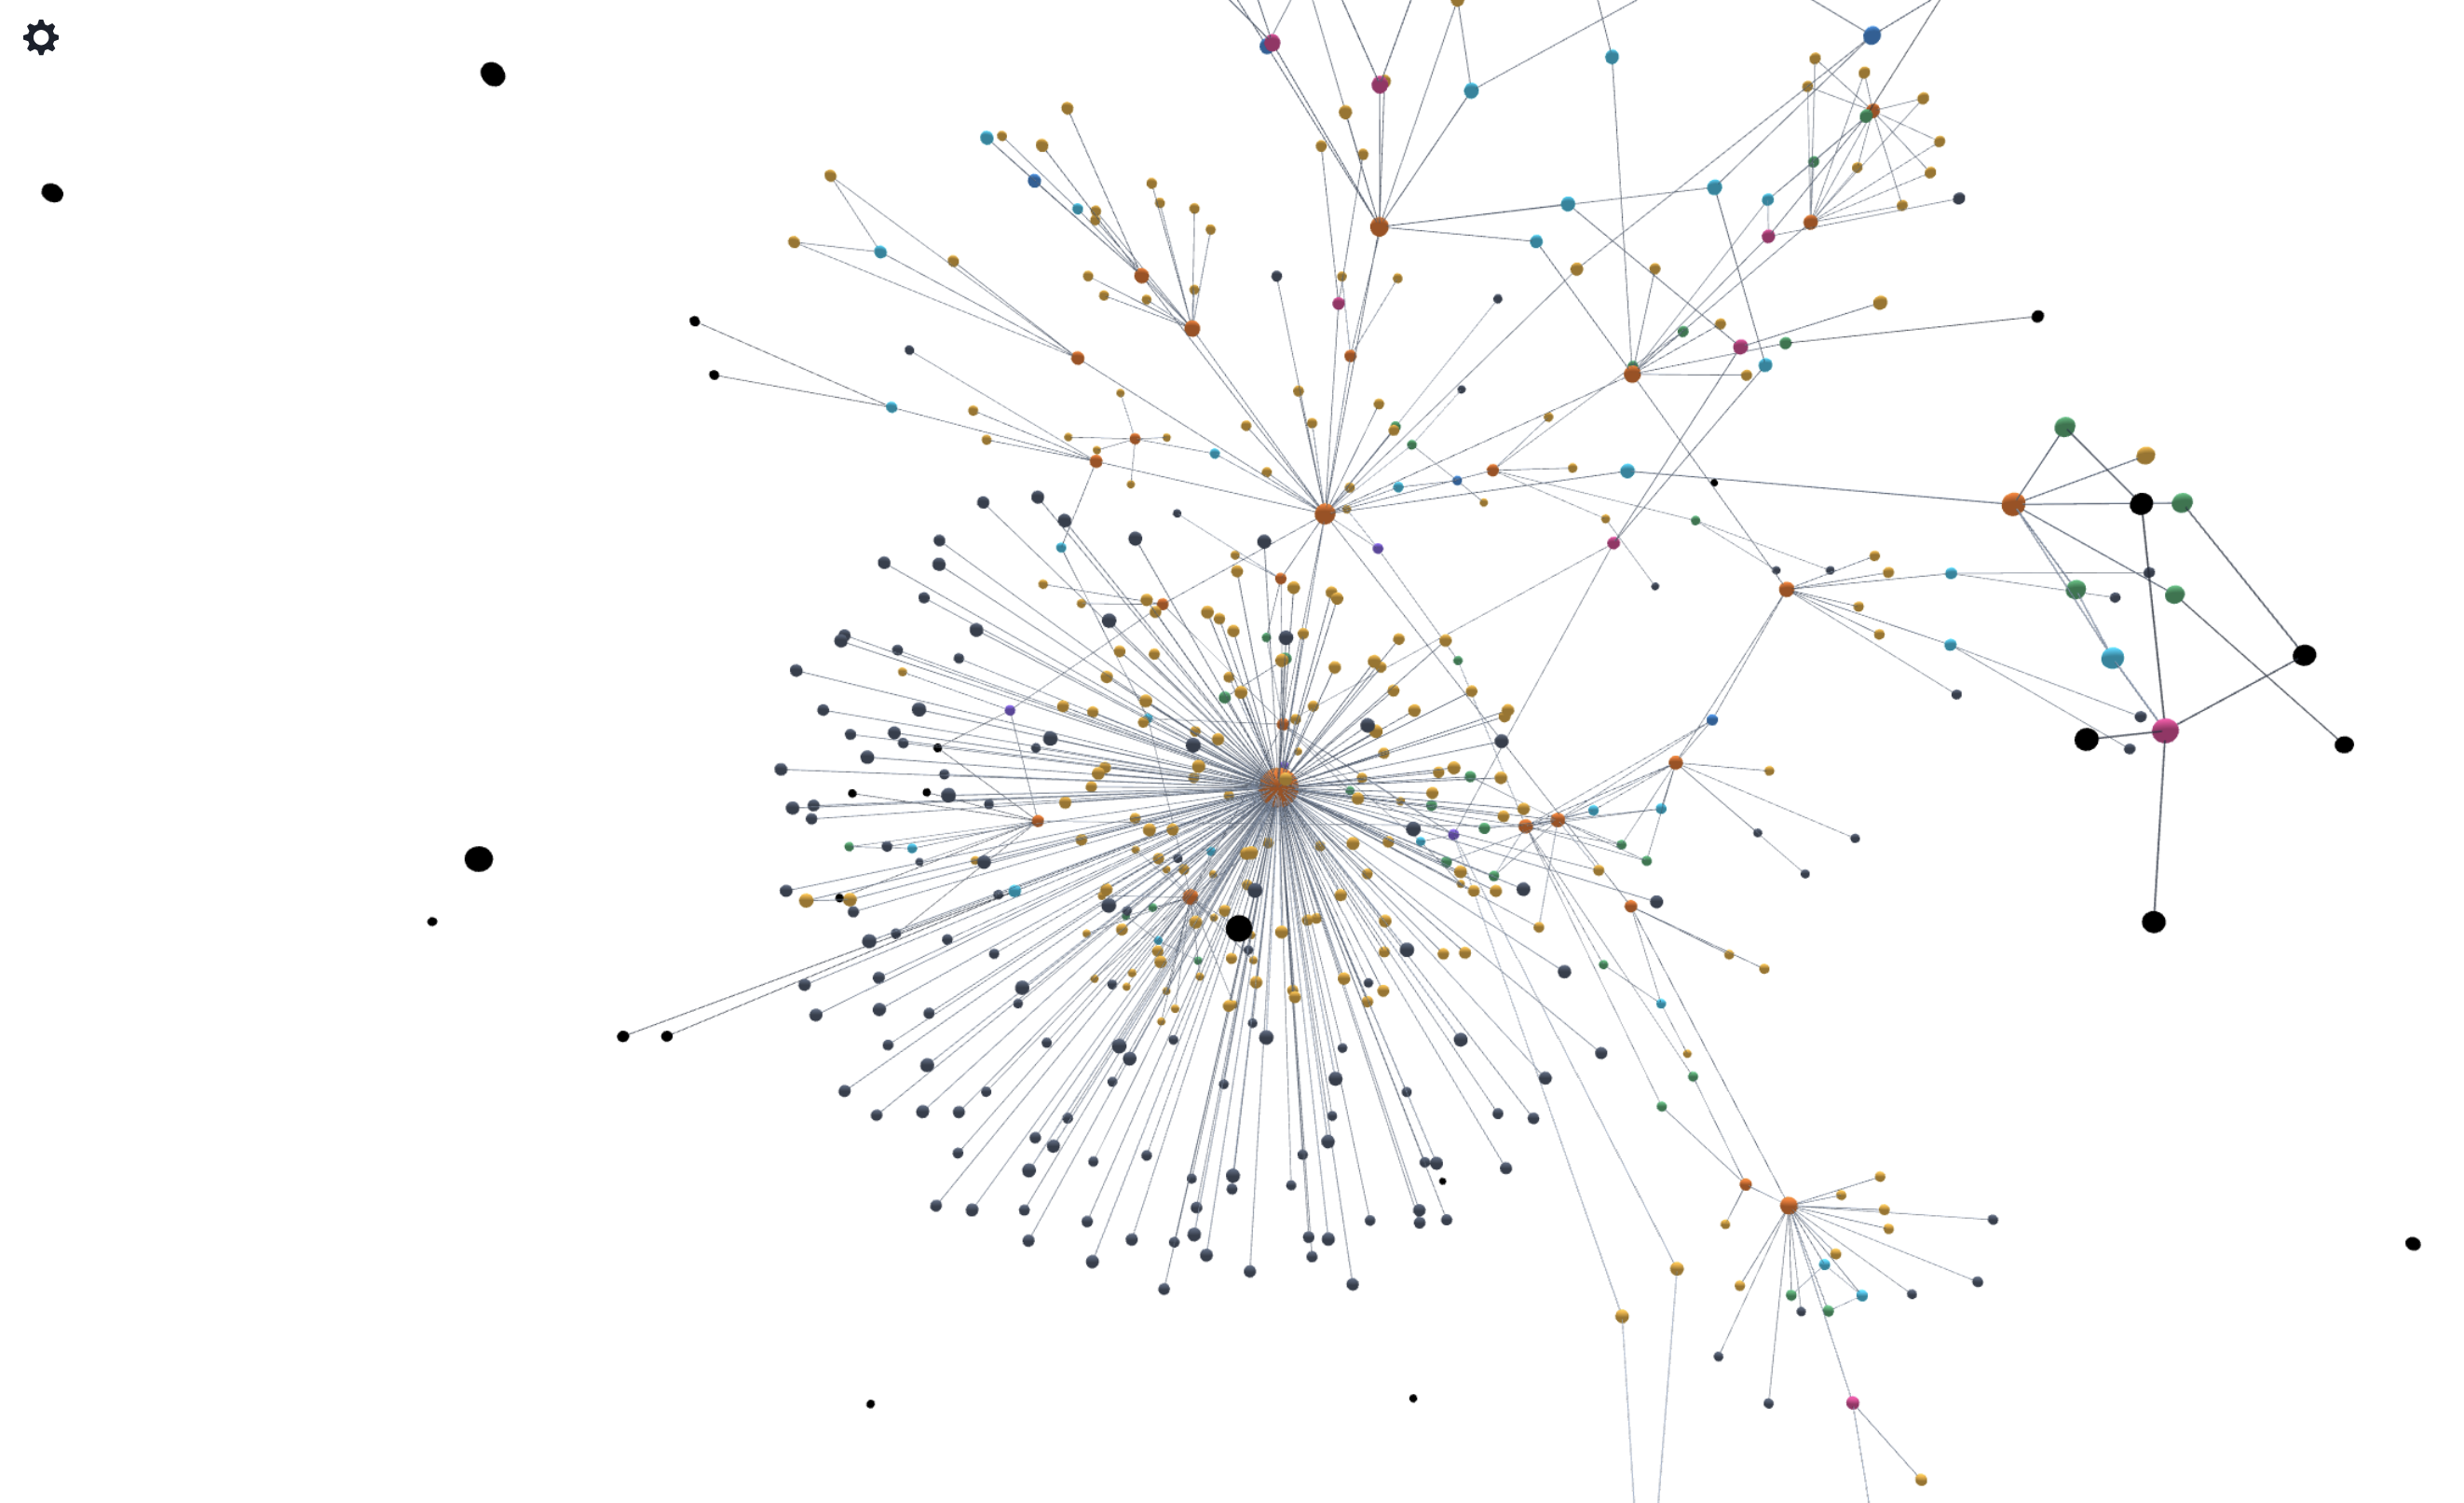
\includegraphics[scale=0.25]{Figures/myzk.png}
\end{center}
\end{frame}

% \section{Closing}

\subsection{More information about Emacs}
\begin{frame}                                             
\frametitle{Books about Emacs}
\begin{center}
    
\includegraphics[scale=0.35]{Figures/EmacsBooks.png}
\end{center}
Glickstein (1997) Writing  GNU Emacs Extensions. O'Reilly.
\end{frame}

\begin{frame} 
\frametitle{Web sites (hyperlinks in slides)}
\begin{columns}
\begin{column}{0.48\textwidth}
    \begin{itemize}[font=$\bullet$\scshape\bfseries]
       \item \href{https://github.com/birkenkrahe/org/blob/master/emacs/tutorial.org}{Marcus' tutorials on Emacs}
       \item \href{https://orgmode.org/worg/}{Org-mode worg link}
       \item \href{https://www.emacswiki.org}{Emacs Wiki}
       \item \href{https://melpa.org/#/}{MELPA}
       \item \href{https://planet.emacslife.com/}{Planet EmacsLife }
       \item \href{https://sachachua.com/blog/2024/11/2024-11-18-emacs-news/}{Sacha Chua's weekly newsletter}
       \item \href{https://github.com/emacs-tw/awesome-emacs}{Awesome Emacs}
        \item GitHub \verb|/emacs|, 47.9 K repositories
    \end{itemize}
\end{column}
\begin{column}{0.48\textwidth}
    \begin{itemize}[font=$\bullet$\scshape\bfseries]
     \item \href{https://www.youtube.com/@JakeBox0}{Jake Boxerman YT, Columbia U student}
     \item \href{https://www.youtube.com/@JohnKitchin}{John Kitchin (Org-ref, Scimax) YT }
     \item \href{https://www.youtube.com/@GavinFreeborn}{Gavin Freeborn YT}
     \item \href{https://www.youtube.com/@SystemCrafters}{Dave Wilson's System Crafters YT}
     \item \href{https://www.youtube.com/@protesilaos}{Protesilous 'Prot' Stravou YT}
     \item \href{https://emacsconf.org/}{Emacsconfs (~160 h of on-line content, 2013, 2015, 2019-2023, Dec. 7 and 8 2024)}
    \end{itemize}
\end{column}
\end{columns}
\end{frame}


\subsubsection{Packages installed by straight}
\begin{frame}
\frametitle{Packages auto installed by straight }
\begin{center}
    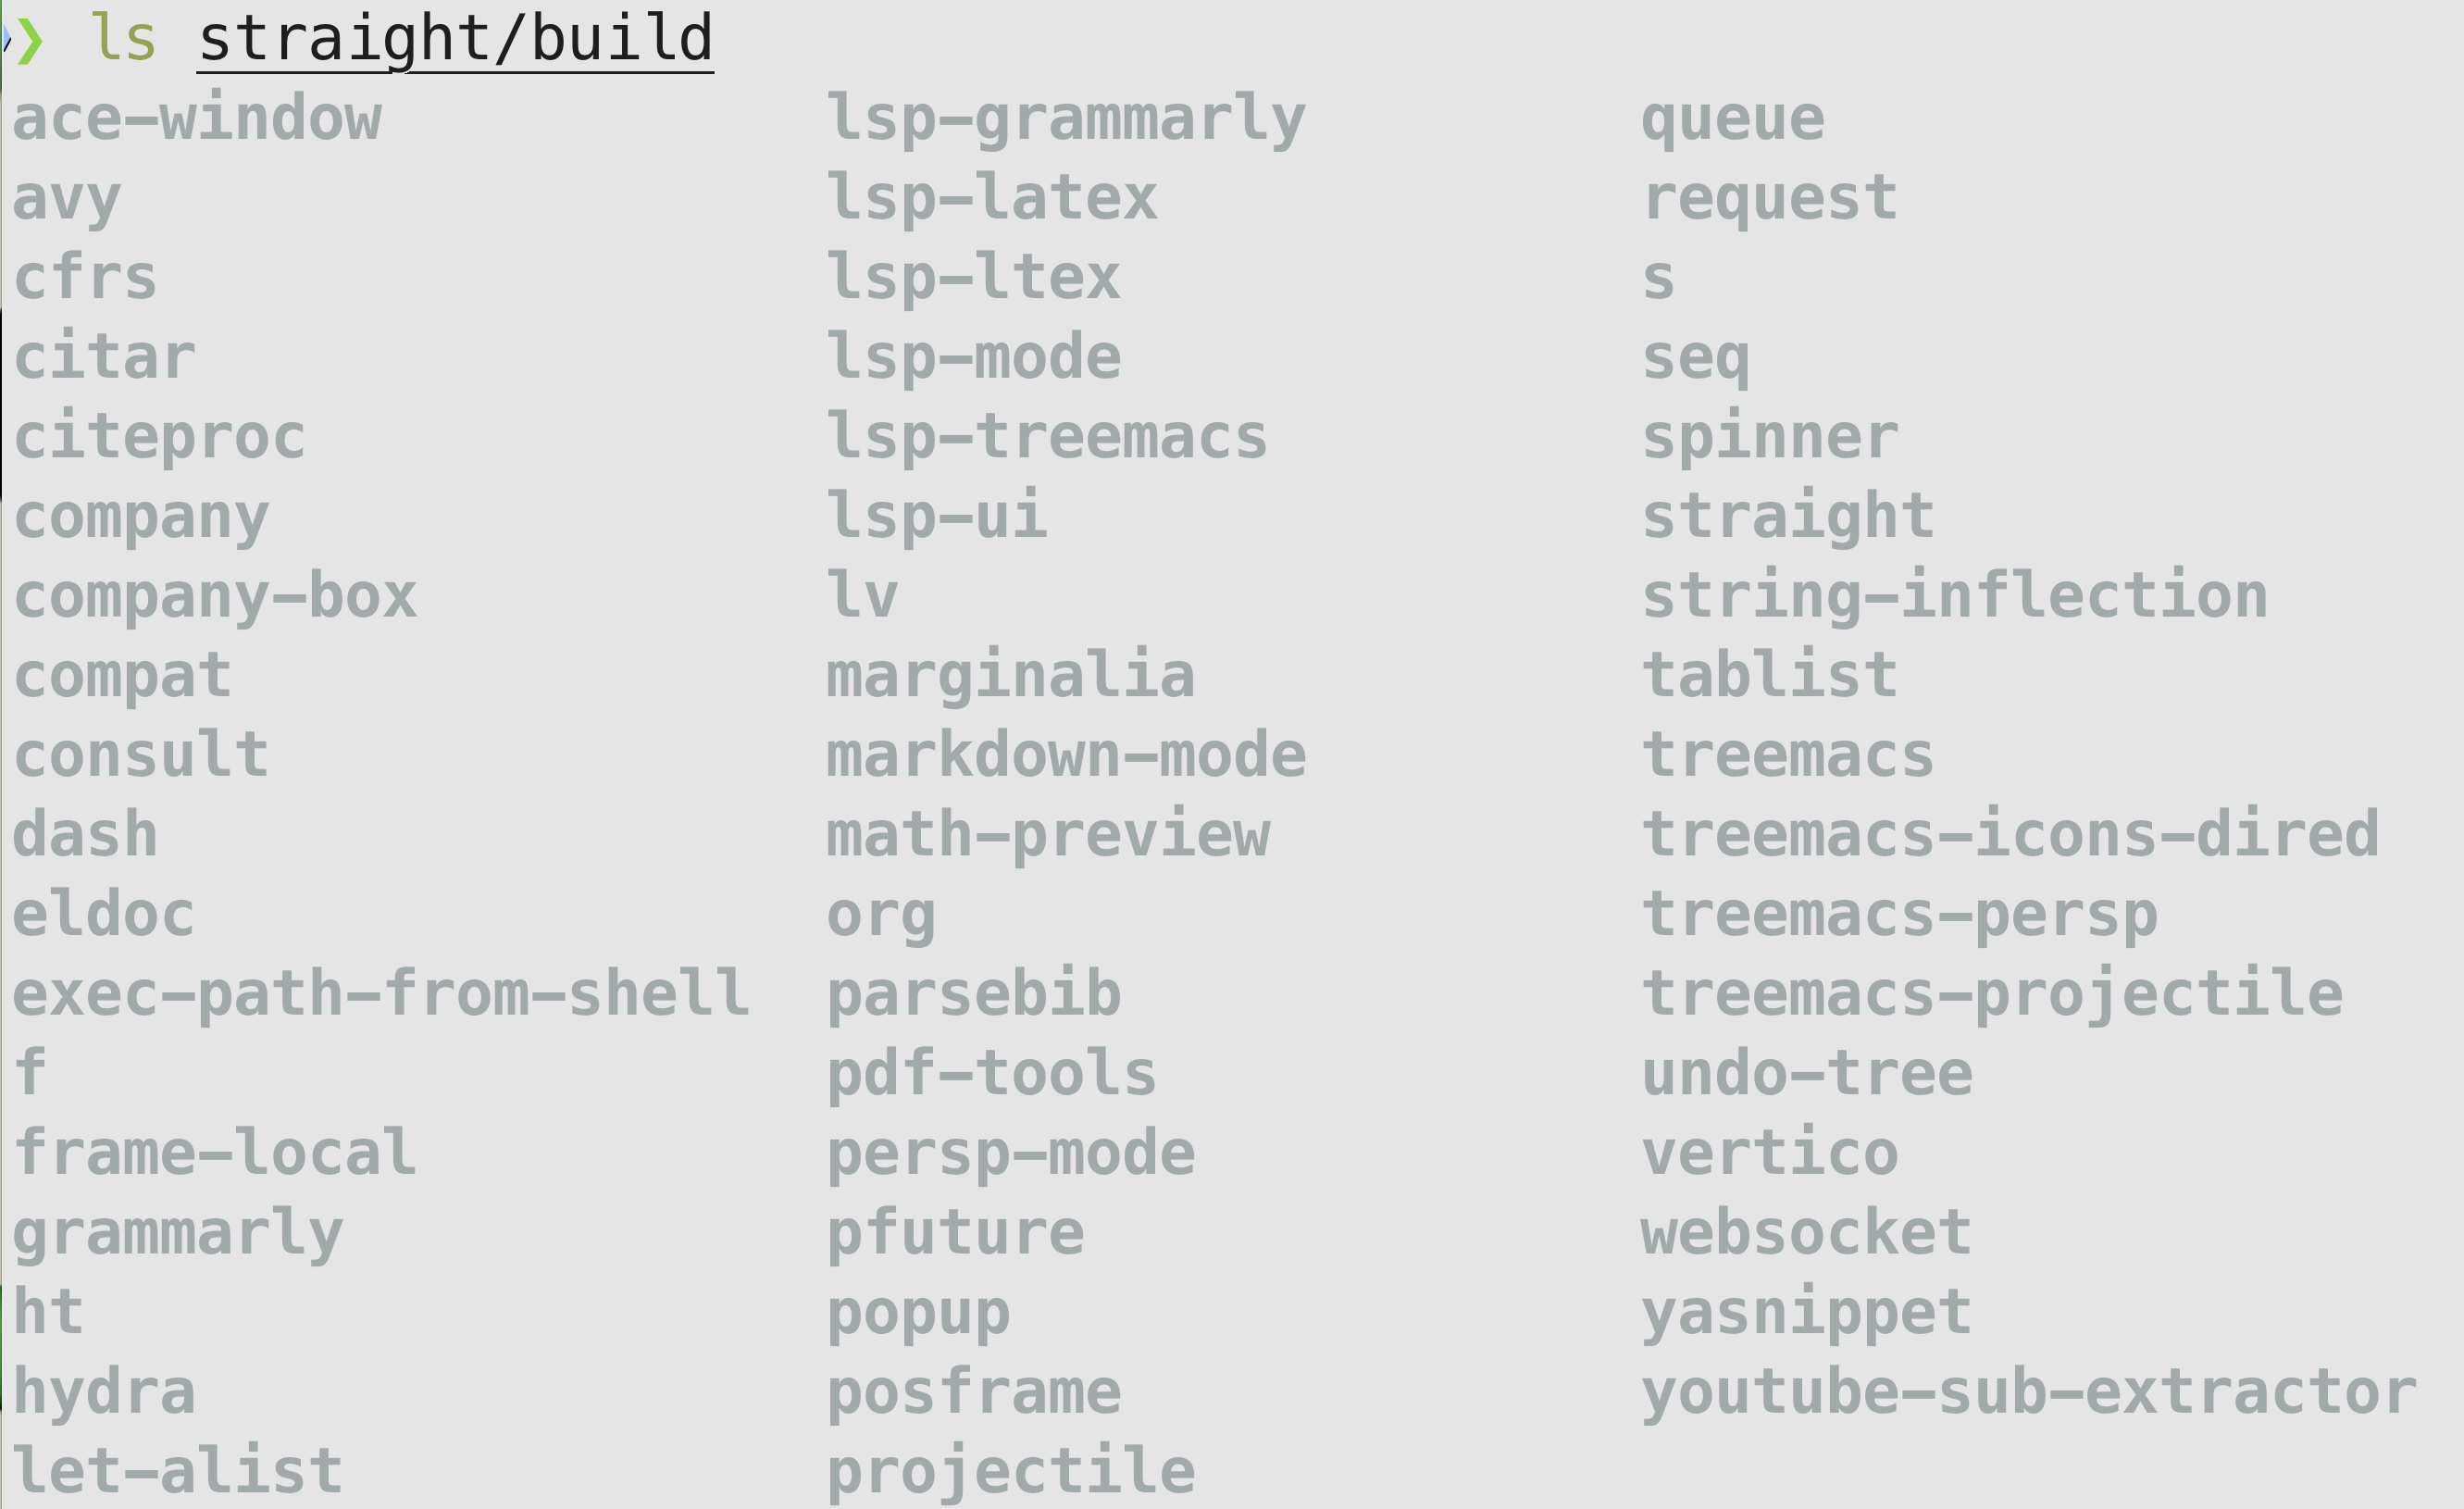
\includegraphics[scale=0.23]{Figures/build.png}
\end{center}
emacs -Q ;; Start Emacs without packages.
\end{frame}

\subsubsection{Opening an orgfile 10-minute demo with org}

\begin{frame}
\frametitle{Demo with new org file}
\begin{center}
\Large{
\begin{itemize}[font=$\bullet$\scshape\bfseries]
\item header section
\item headlines
\item folding and expanding with tab
\item shuffling of items in lists
\item shuffling of sentences written OSPL
\item table creation
\item using LaTeX directly and with keywords
\item opening images in adjacent buffers
\end{itemize}
}
\end{center}
\end{frame}
% Live demo of key features -- 10 minutes



% % \subsection{More information about Org-mode}
% % \begin{frame}
% % \frametitle{More information about Org-mode}
% % \end{frame}

% \subsection{More information about Zettelkastens and org-roam}
% \begin{frame}
% \frametitle{Books on Zettelkastens}
% \begin{center}
%     
\includegraphics[scale=0.35]{Figures/ZKbooks.png}
% \end{center}
% \end{frame}

% \subsection{Books on Science Writing}
% \begin{frame}
% \frametitle{Books on Science Writing}
% \begin{center}
%     
\includegraphics[width=0.99\textwidth, angle=0]{./Figures/fourBooks.png}
% \end{center}
% \end{frame}
% \note{
% The writing Project Specific log that I will be presenting is more of a thinking tool than an accountability tool.
% I have not seen it described you in the limited number of books I have read about scientific writing.
% Here are four of my favorite books.
% Ivory Paul Silver's book how to write a lot whenever I am in a slump because he is very effective at pointing out that you really have to schedule your writing effort much in the way that you schedule the preparation of lectures.
% The second book is the source of the accountability form of the writing log.
% The third book is the origin of my approach to organizing and assembling a good part of a manuscript and a single day. It is by the Australian David Lindsey and then the last book is one that I am still reading and spy Stephen B. Heard with. It is very well written and it is expresses I think the state of the art in terms of the approach that most productive scientist take to writing.
% }

\subsubsection{The problem}
\defverbatim[colored]\exampleCodeC{
\large{
\begin{pythoncode}
    install mpv (Homebrew, MacPorts, yum, etc.)
    sudo curl -L https://yt-dl.org/downloads/latest/youtube-dl\
         -o /usr/local/bin/youtube-dl
    sudo chmod a+rx /usr/local/bin/youtube-dl

    (defun play-youtube-video (url)
      "Play a YouTube video with mpv."
      (interactive "sYouTube URL: ")
      (start-process "mpv" nil "mpv" URL))C-x C-e in scratch buffer

    Minibuffer:
    M-x play-youtube-video 
\end{pythoncode}
}
}
% Slide 24
\begin{frame}
\frametitle{Elisp function to play YouTube video in MPV}


\exampleCodeC
\end{frame}


\end{document}
